\documentclass{article}
\usepackage{amsmath}
\usepackage{graphicx}
\usepackage{caption}
\usepackage{subcaption}

\begin{document}
\section{Numerical Methods}\label{sec:Numerical Methods}

%%%%%%%%%%%%%%%%%%%%%%%%%%%%%%%%%%%%%%%%%%%%%%%%%%%%%%%%%%%%%%%%%%%%%%
\subsection{Asset Collision Algorithm}\label{ssec:Asset Collision Algorithm}

In this lunar ejecta model, the asset is assumed to be cylindrical in shape with the cylinder's symmetry axis normal to the lunar surface. The asset can sit on the surface of the Moon or have any height above the surface, $h_{sb}$ such that
\begin{equation}
h_{sb} = r_s - r_m.
\end{equation}
The height (or length) of the asset itself is defined to be $l_s$, so that the height of the top of the asset from the lunar surface is given by
\begin{equation}
h_{st} = h_{sb} + l_s.
\end{equation}
The radius of the cylinder is defined to be $a_s$.

In order to uniformly\footnote{A constant probability density in the speed-zenith-azimuth phase space.} generate ejecta that originates from a crater and will hit the asset, there are bounding points that define the extent of the minimum and maximum ejecta speed ($v_{min,\gamma_p}$ and $v_{max,\gamma_p}$) for a given ejecta zenith and azimuth angle. It is assumed that for speeds $v_p$ such that $v_{min,\gamma_p} \le v_p \le v_{max,\gamma_p}$, the $(v_p, \gamma_p)$ pair gives ejecta that will hit the asset. The question then becomes, where?

Given the ejecta speed $v_p$, zenith angle $\gamma_p$, selenographic distance to the near side of the asset $D$, in addition to the asset height above the lunar surface and the size, the height $r_s$ and distance $D_s$ at which the ejecta hits the asset is needed. To know which surface the ejecta hits (top, side, bottom), the state of the ejecta at the distance $D$ is needed, specifically the height $r_s(D)$ using Equation \eqref{eq:rs}. To decide which surface of the asset is hit by the ejecta, the following logic can be used:
\begin{itemize}
	\item If $r_s(D) > h_{st}$, then $sign(F) = -1$, $r_s = h_{st}$, and $D_s = D(v_p, \gamma_p, r_s)$ (hitting the top),
	\item Else if $r_s(D) < h_{sb}$, then $sign(F) = +1$, $r_s = h_{sb}$, and $D_s = D(v_p, \gamma_p, r_s)$ (hitting the bottom),
	\item Else
	\begin{itemize}
		\item If $\gamma_p > \gamma_{p,ap}(r_s(D))$ (Equation \eqref{eq:gamma p ap 1}), then $sign(F) = -1$, $r_s = r_s(D)$, and $D_s = D$ (hitting the side above the local horizon),
		\item Else $sign(F) = +1$, $r_s = r_s(D)$, and $D_s = D$ (hitting the side below the local horizon).
	\end{itemize}
\end{itemize}
For computing both $F$ and $D$, the conditionally defined height $r_s$ and sign of $F$ should be used.

Examples of valid ejecta from a crater that hits various asset sizes are shown in Figures \ref{fig:asset_speed_zenith_comparison}, \ref{fig:asset_speed_zenith_comparison_h1}, and \ref{fig:asset_speed_zenith_comparison_h1} for asset altitudes of $0r_m$, $0.01r_m$, and $0.1r_m$, respectively. For each figure, the asset properties are ($a=0.01r_m$, $h=0.2r_m$) for the left column, ($a=0.01r_m$, $h=0.02r_m$) for the center column, and ($a=0.1r_m$, $h=0.02r_m$) for the right column. The crater-to-asset distance varies for the rows, where row 1 is $D=0.002r_m$, row 2 is $D=0.02r_m$, row 3 is $D=0.2r_m$, and row 4 is $D=2.0r_m$.

For an asset on the surface of the Moon (Figure \ref{fig:asset_speed_zenith_comparison}), there are no ejecta that hit the bottom of the asset -- which is to be expected. When a crater is close to the asset (rows 1 and 2 of Figure \ref{fig:asset_speed_zenith_comparison}), most of the ejecta hits the asset at the side and occurs for all speeds line-of-site ejecta that are able to reach the bottom edge of the asset.

In general, the further away the crater is from the asset, the more ejecta will hit the top of the asset. For close craters and the higher the asset altitude\footnote{Also, for an asset above the surface of the Moon, several sample points need to be chosen at the bottom surface. The higher the asset, the more points that are needed.}, the more ejecta will hit the bottom of the asset.

% https://tex.stackexchange.com/questions/102251/figures-in-subfigure-not-aligned
\begin{figure}
	\begin{subfigure}[t]{.32\textwidth}
		\centering
		% include first image
		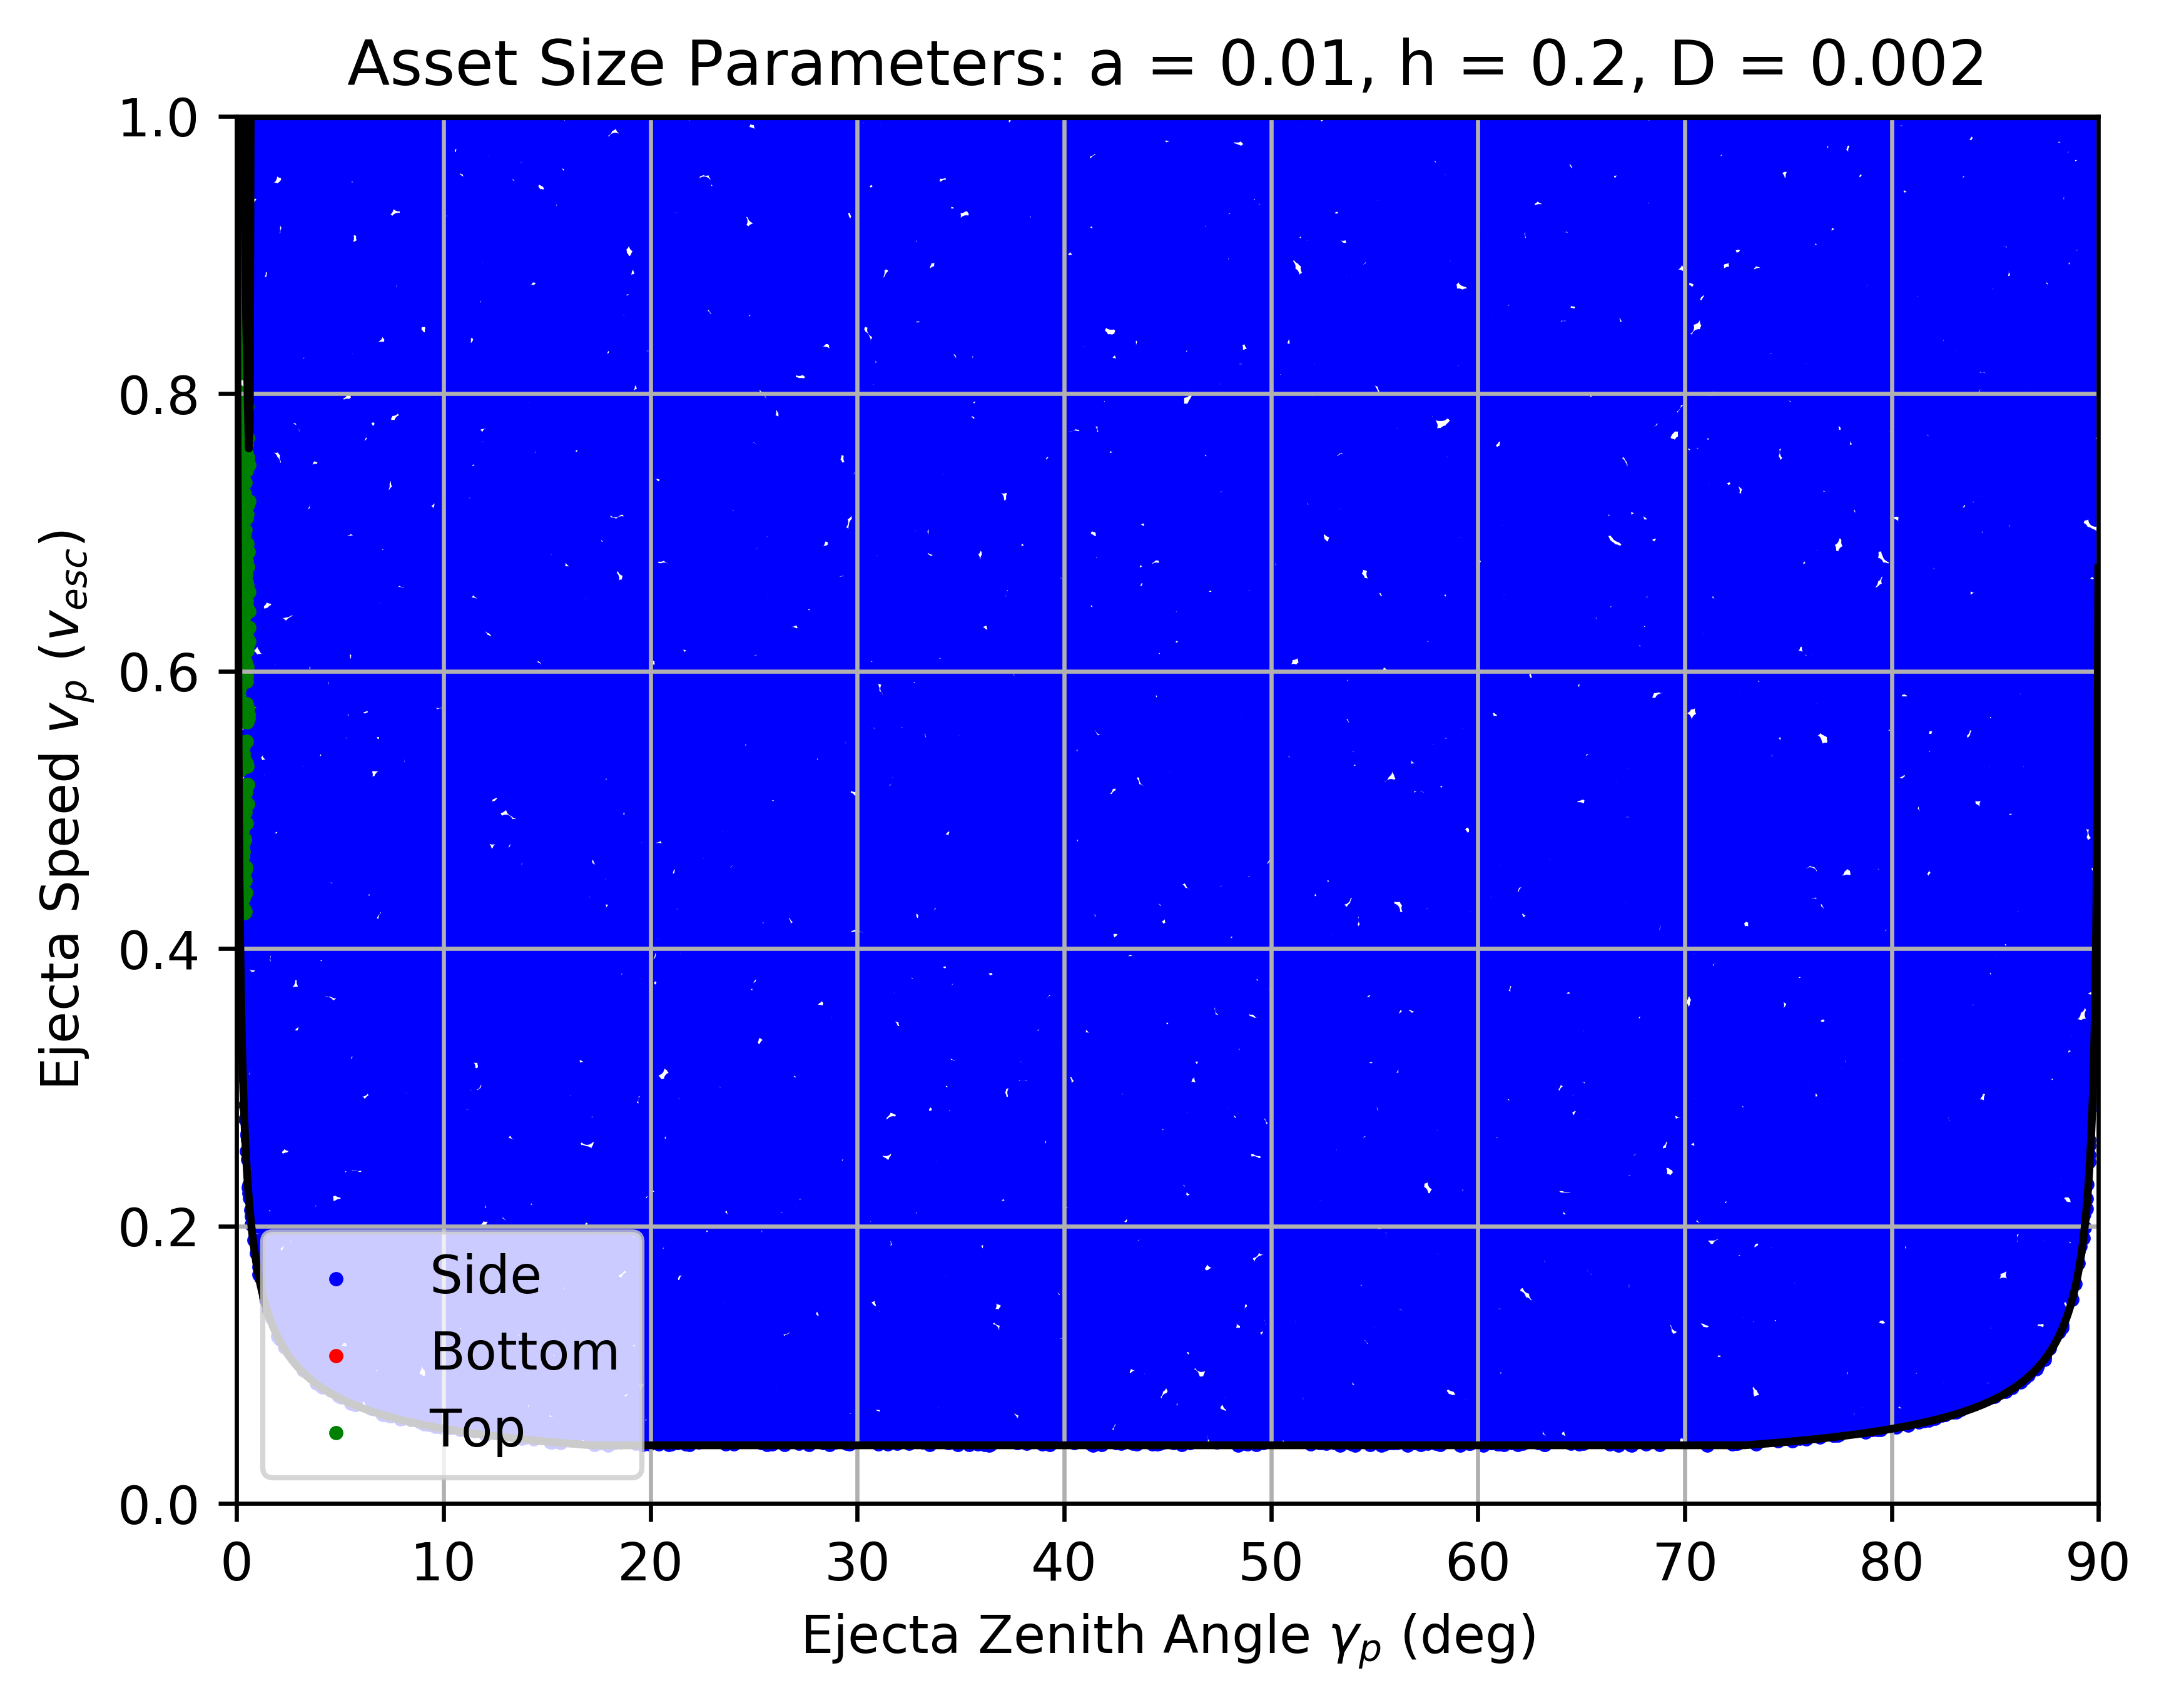
\includegraphics[width=.95\linewidth]{asset_speed_zenith_plot_1.000e-02_2.000e-01_2.000e-03.png}  
		%\caption{Put your sub-caption here}
		\label{fig:sub-asset_speed_zenith_1}
	\end{subfigure}
	\begin{subfigure}[t]{.32\textwidth}
		\centering
		% include second image
		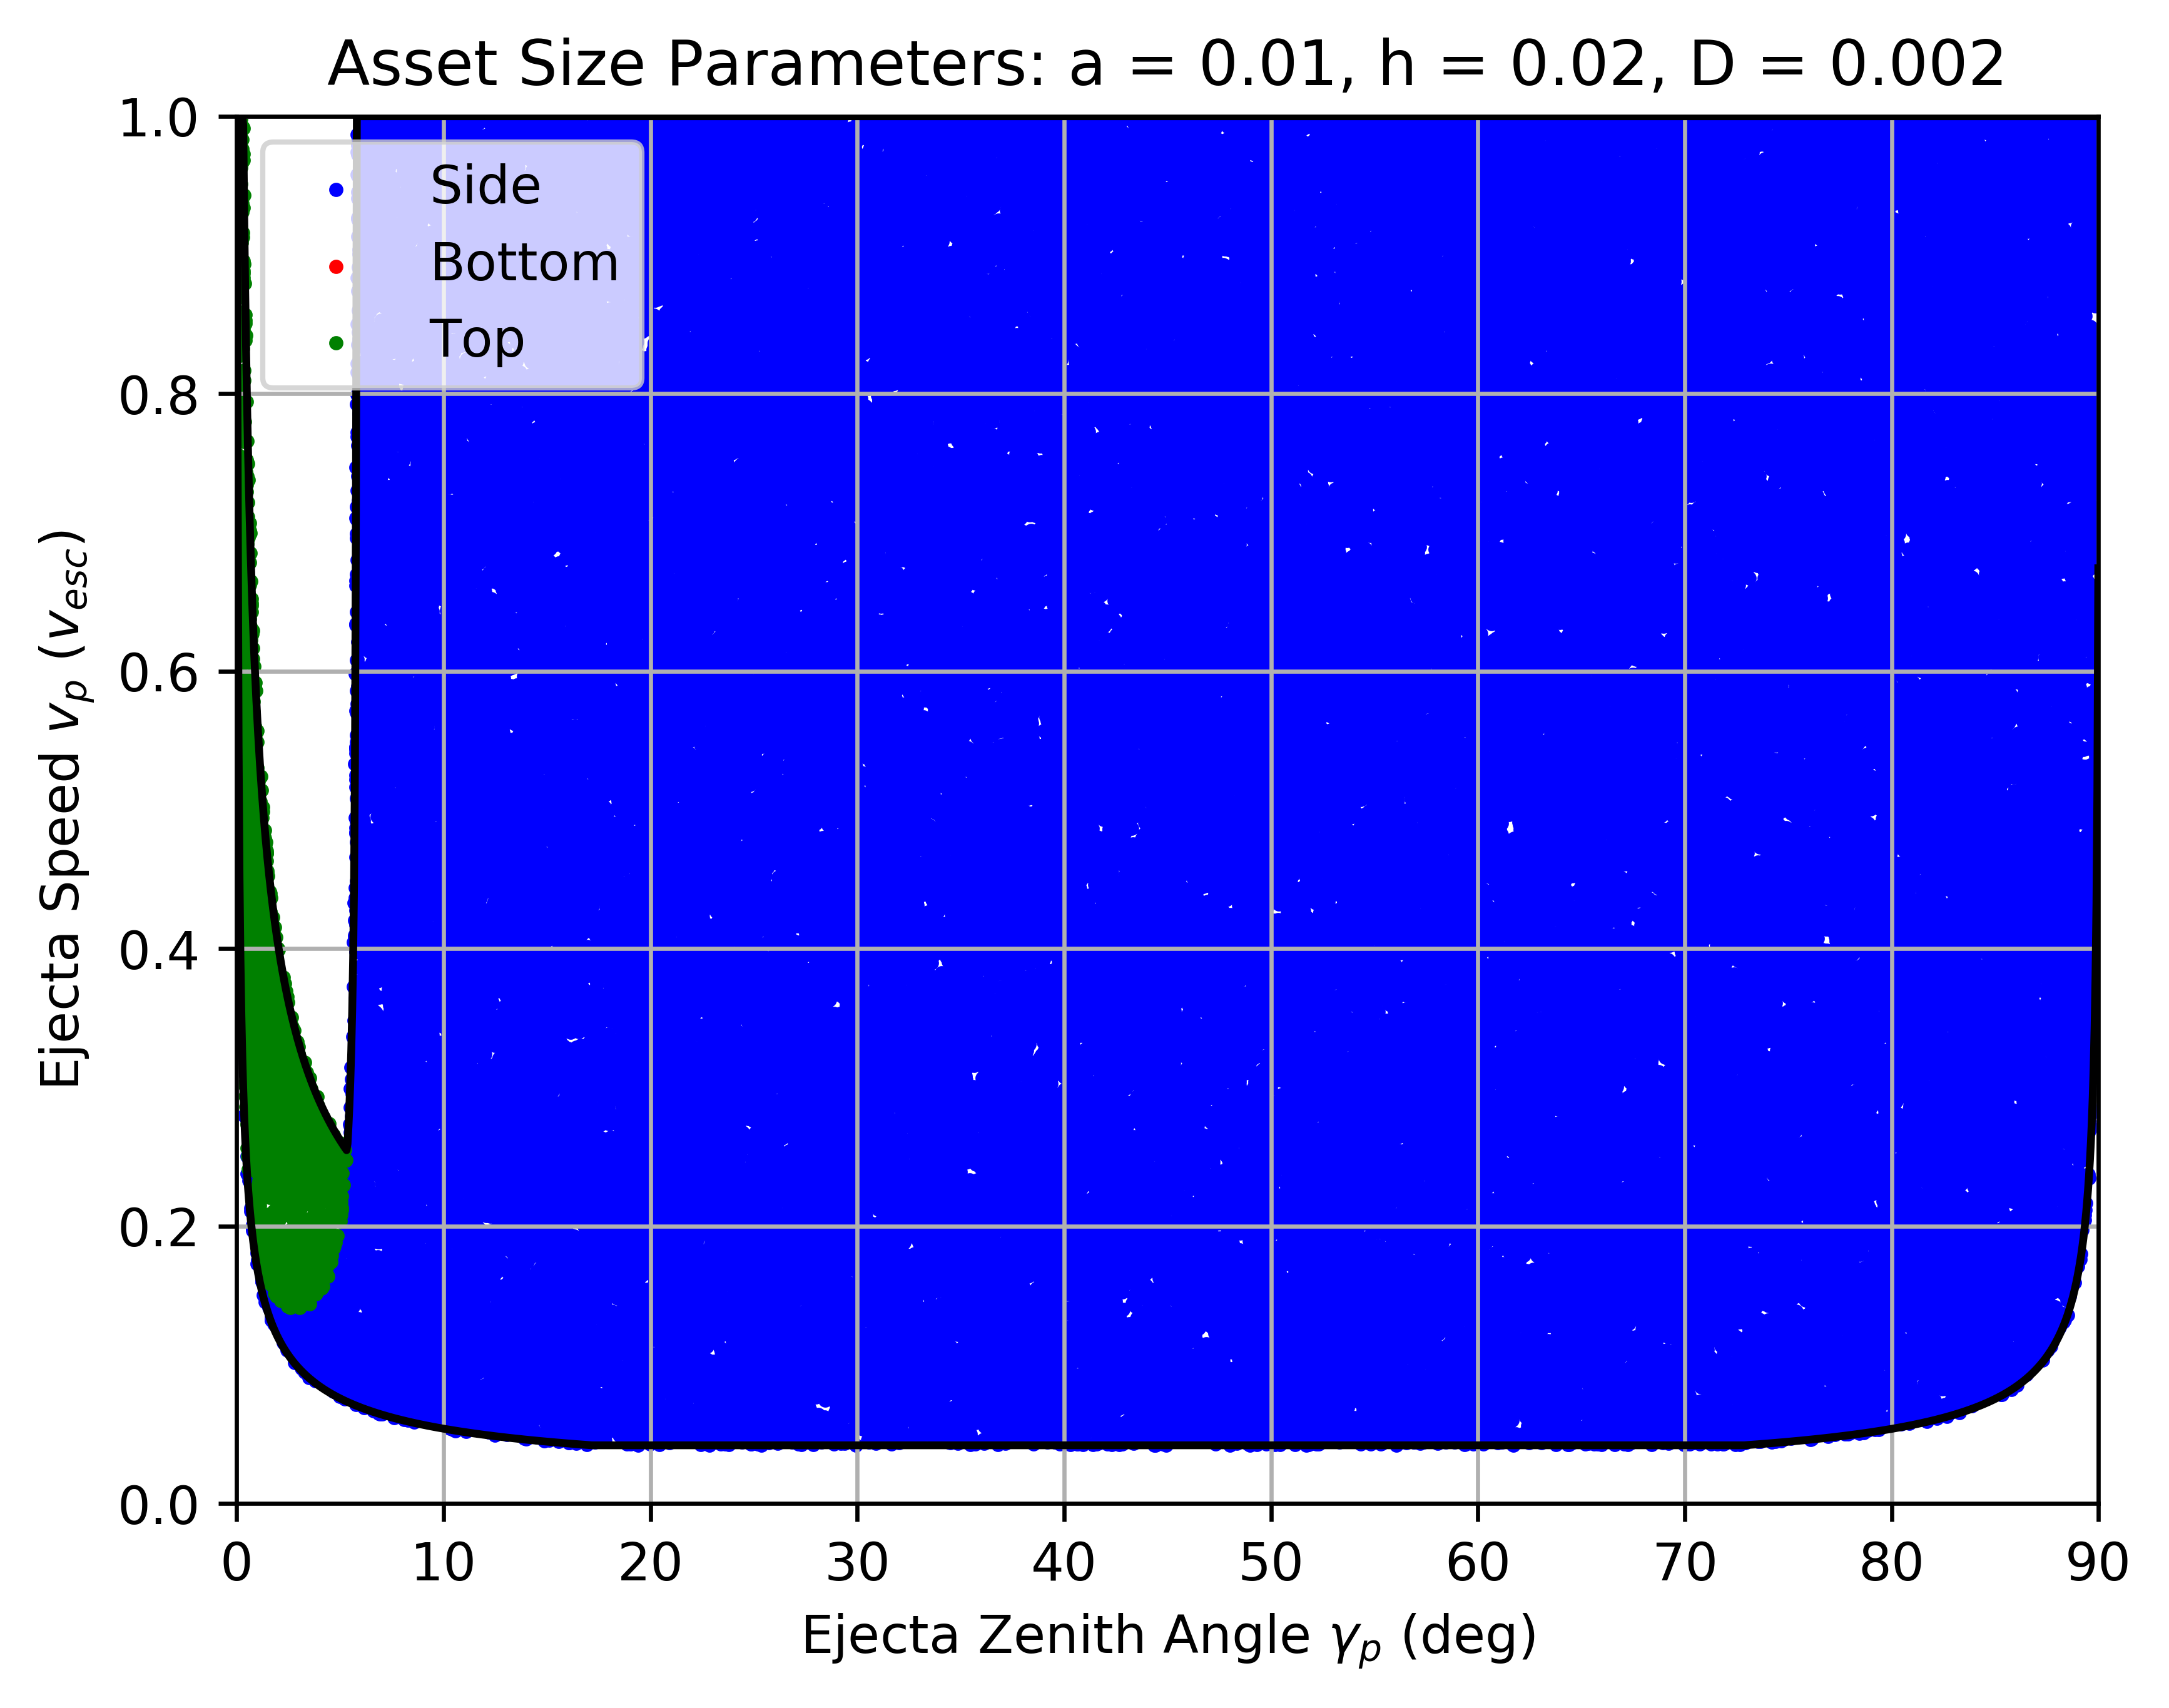
\includegraphics[width=.95\linewidth]{asset_speed_zenith_plot_1.000e-02_2.000e-02_2.000e-03.png}  
		%\caption{Put your sub-caption here}
		\label{fig:sub-asset_speed_zenith_2}
	\end{subfigure}
	\begin{subfigure}[t]{.32\textwidth}
		\centering
		% include second image
		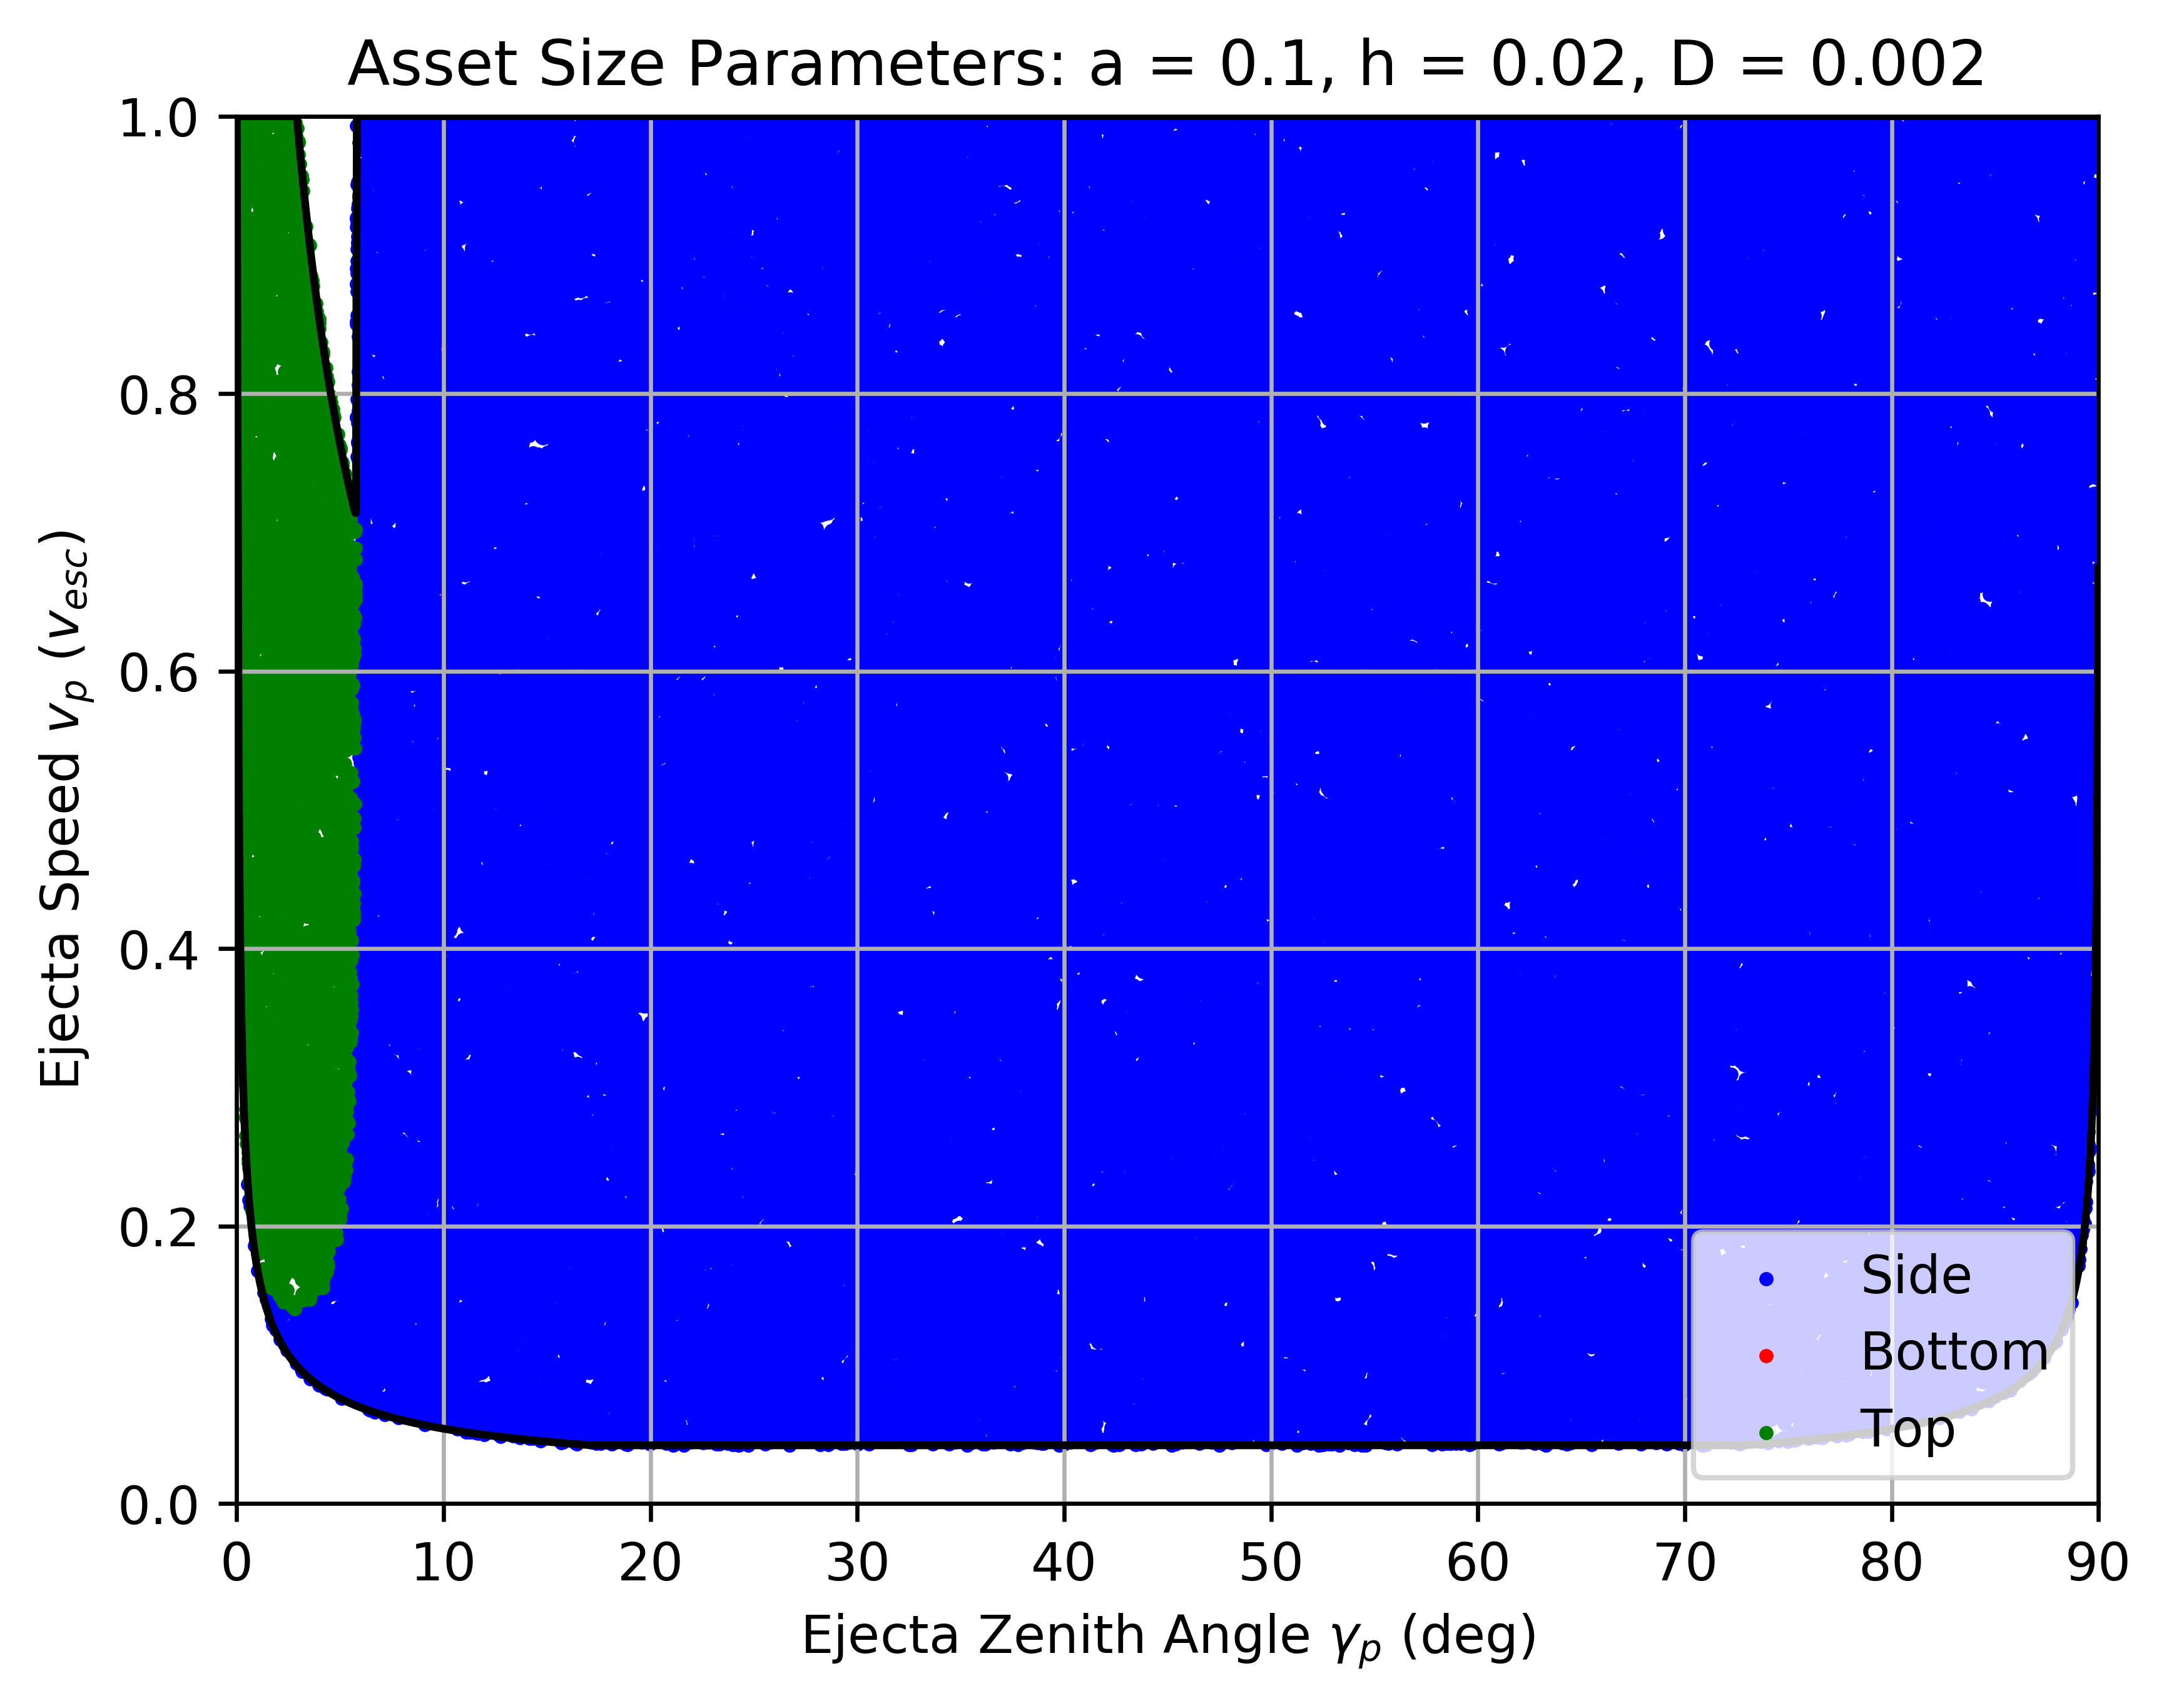
\includegraphics[width=.95\linewidth]{asset_speed_zenith_plot_1.000e-01_2.000e-02_2.000e-03.png}  
		%\caption{Put your sub-caption here}
		\label{fig:sub-asset_speed_zenith_3}
	\end{subfigure}
	
	%\newline
	
	\begin{subfigure}[t]{.32\textwidth}
		\centering
		% include third image
		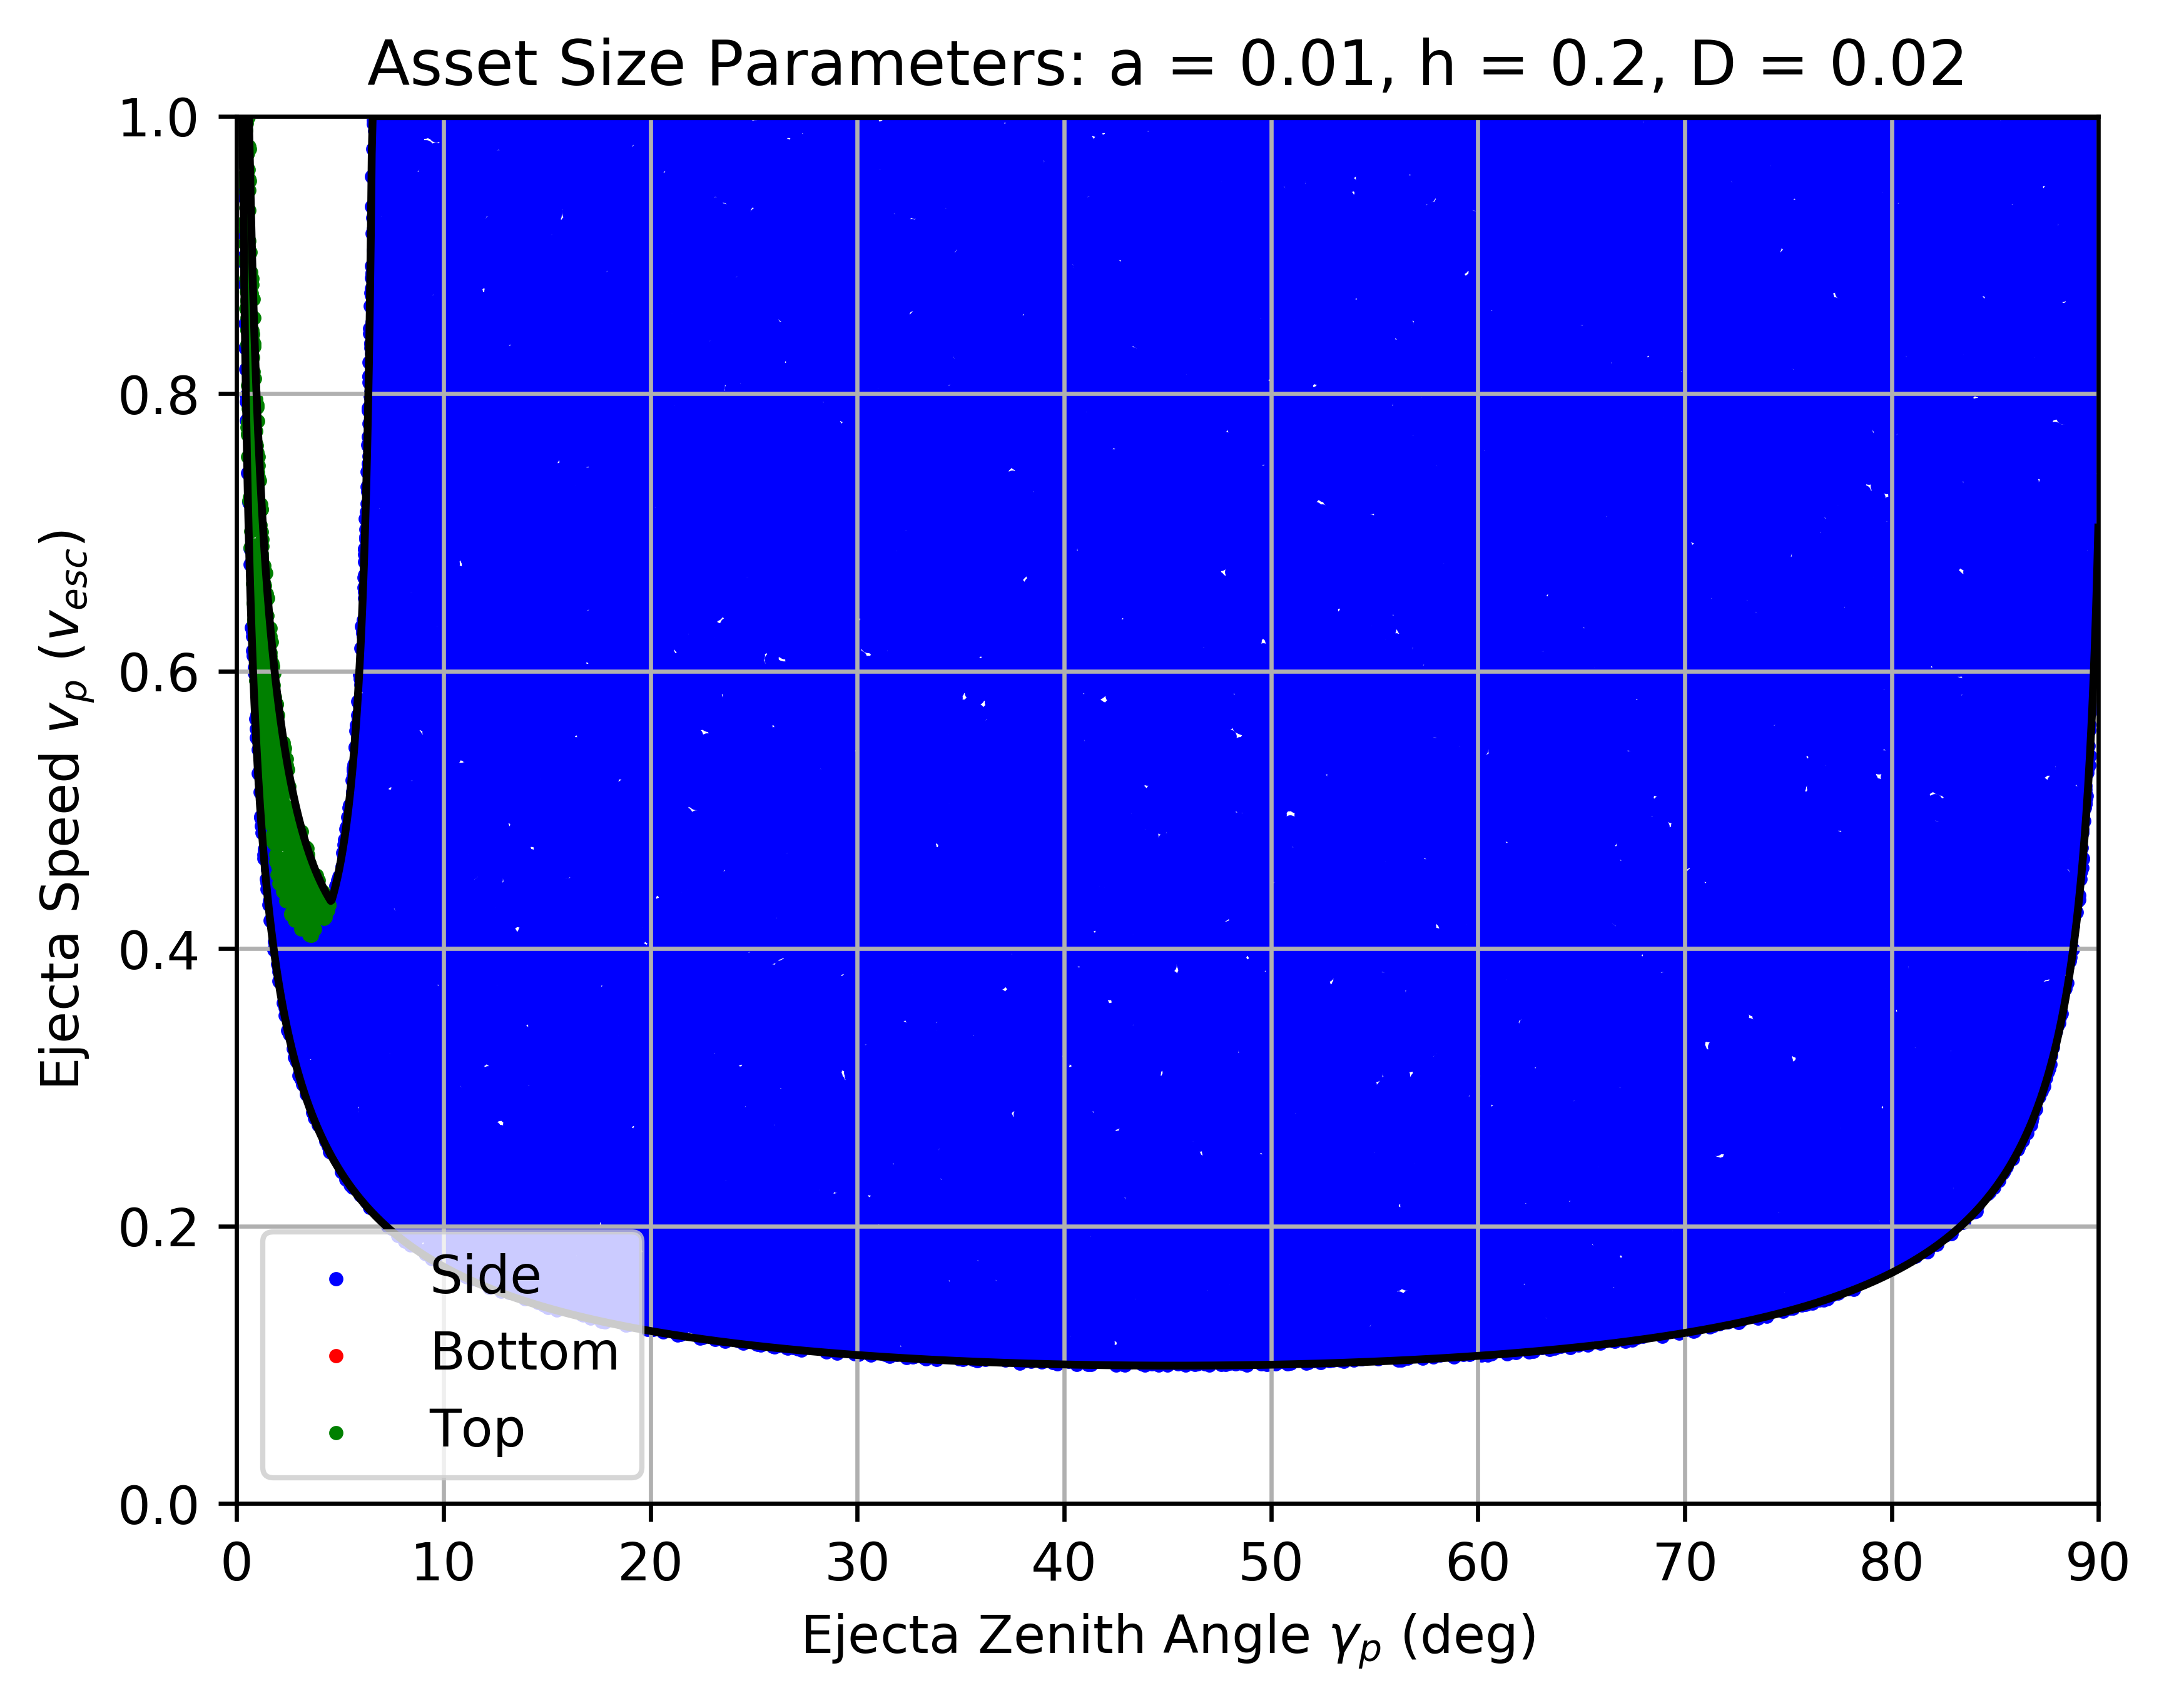
\includegraphics[width=.98\linewidth]{asset_speed_zenith_plot_1.000e-02_2.000e-01_2.000e-02.png}  
		%\caption{Put your sub-caption here}
		\label{fig:sub-asset_speed_zenith_4}
	\end{subfigure}
	\begin{subfigure}[t]{.32\textwidth}
		\centering
		% include fourth image
		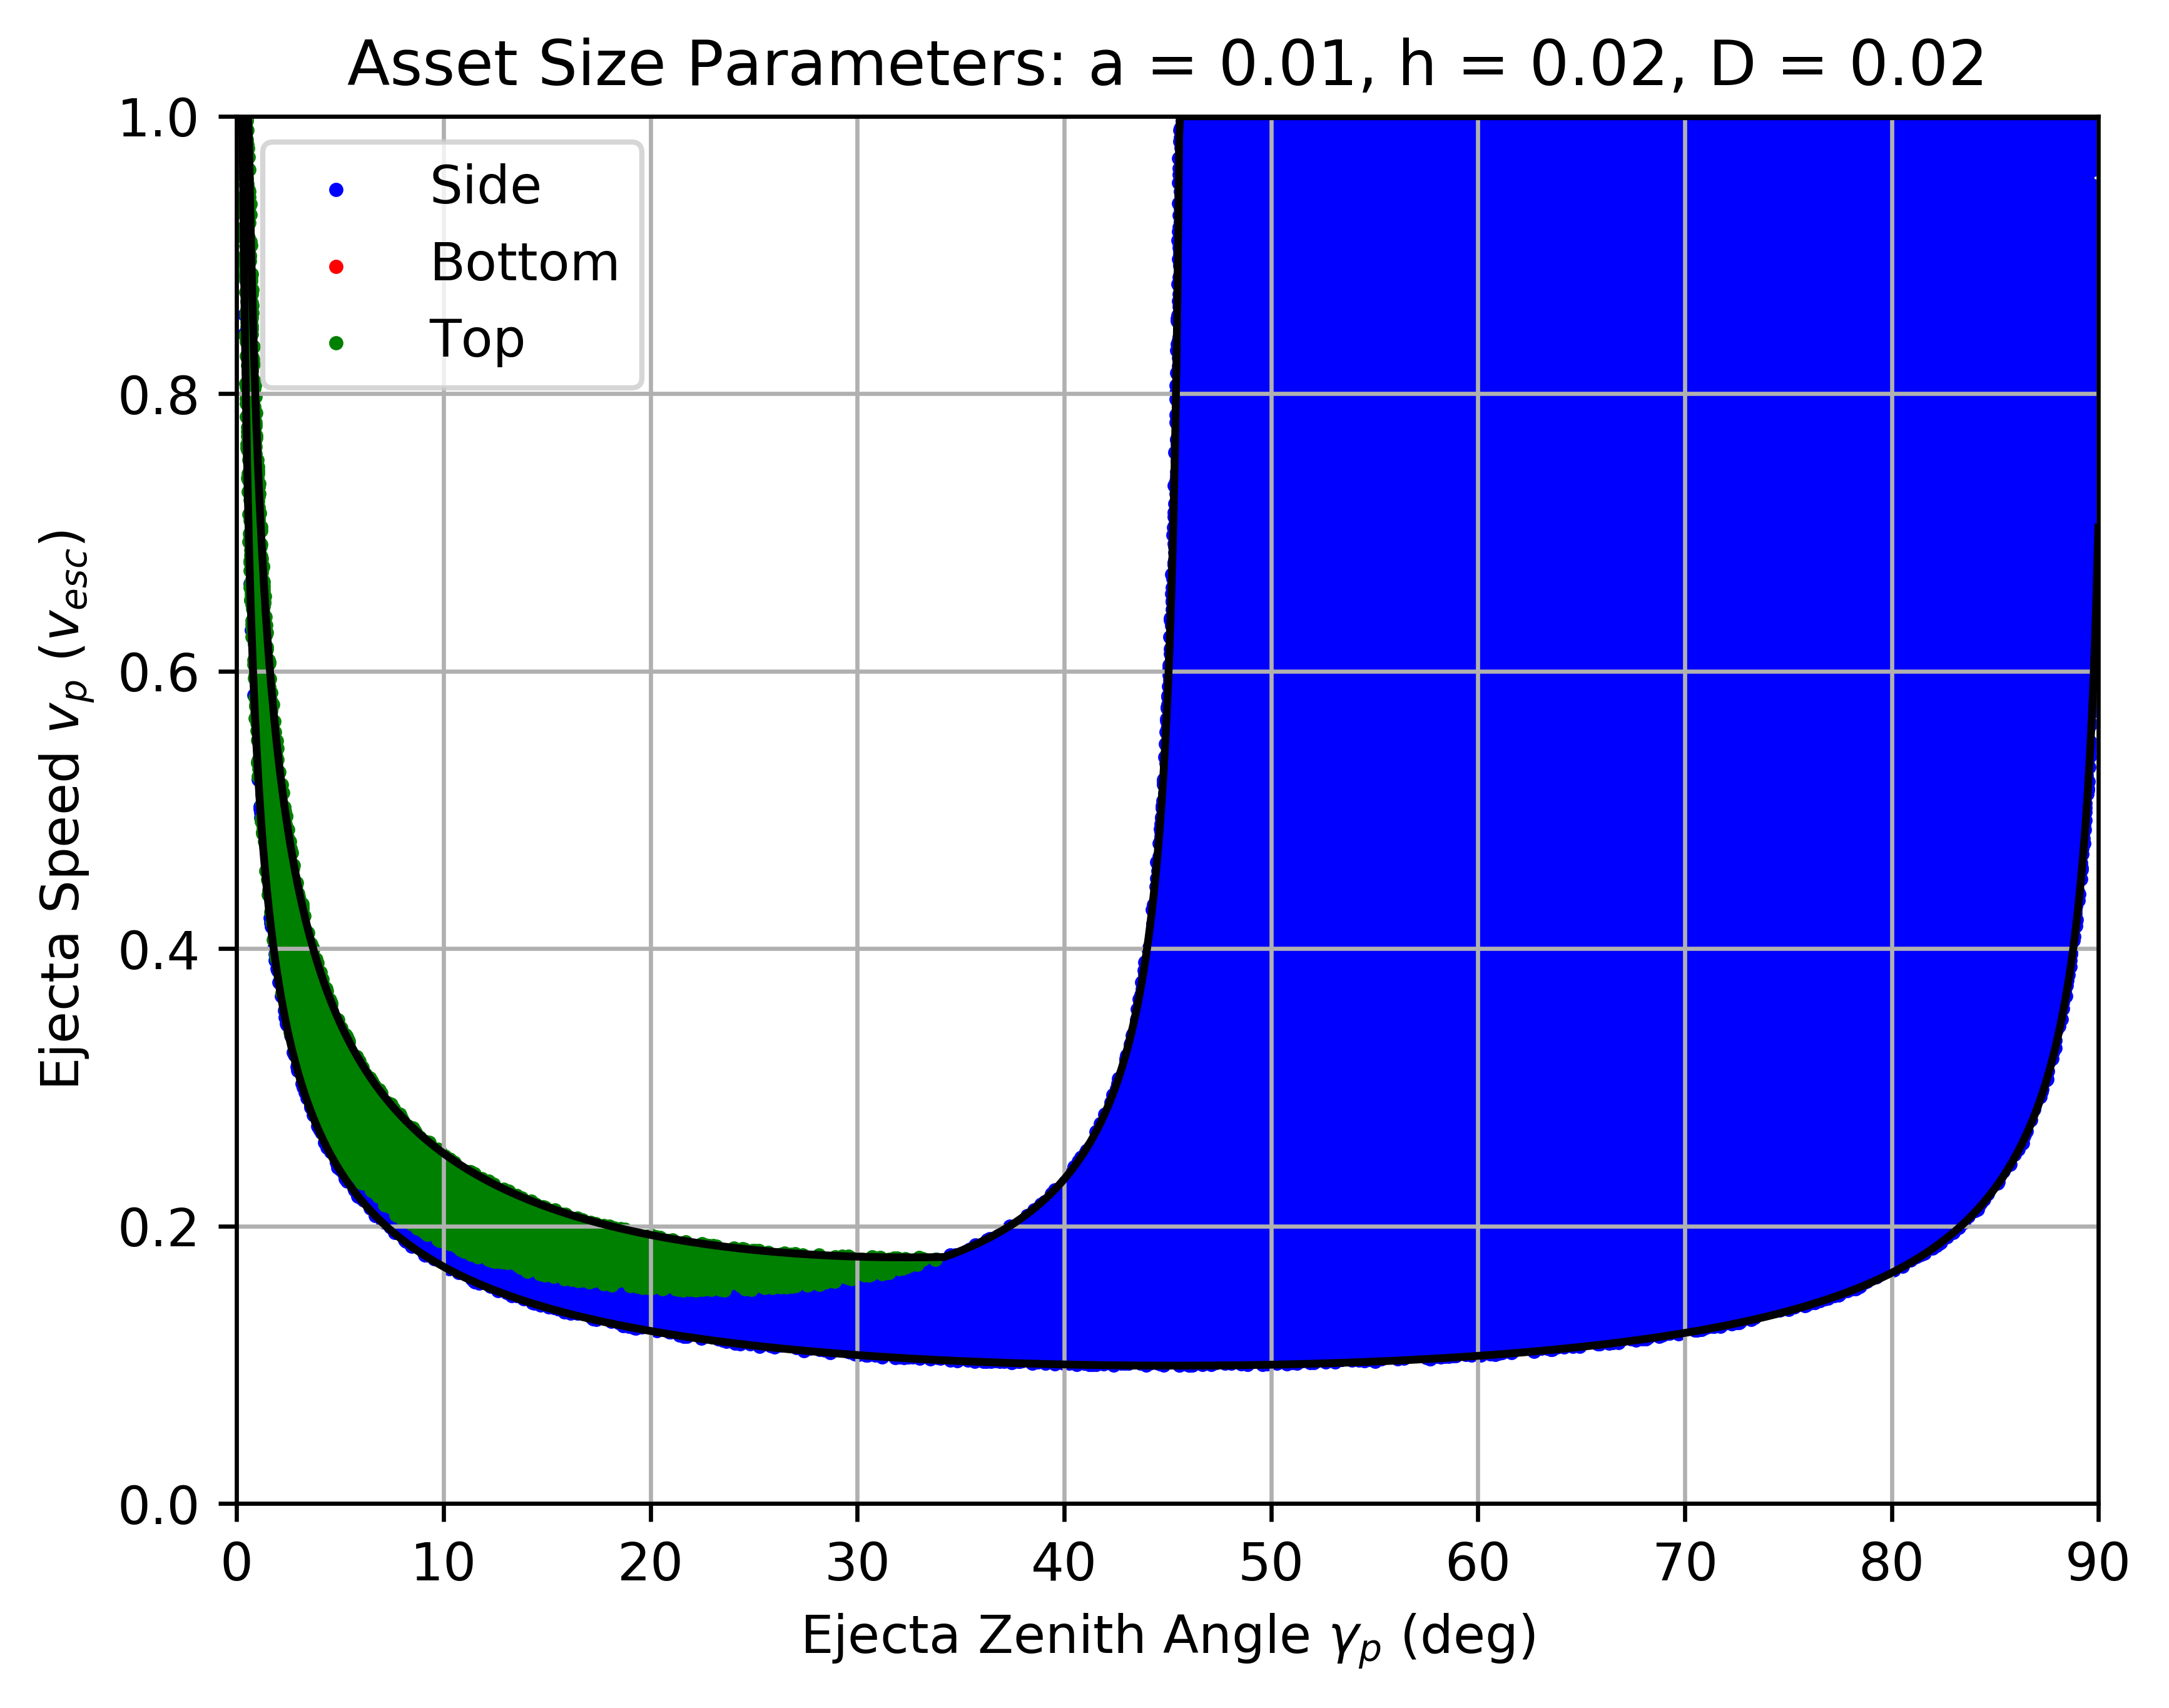
\includegraphics[width=.98\linewidth]{asset_speed_zenith_plot_1.000e-02_2.000e-02_2.000e-02.png}  
		%\caption{Put your sub-caption here}
		\label{fig:sub-asset_speed_zenith_5}
	\end{subfigure}
	\begin{subfigure}[t]{.32\textwidth}
		\centering
		% include fourth image
		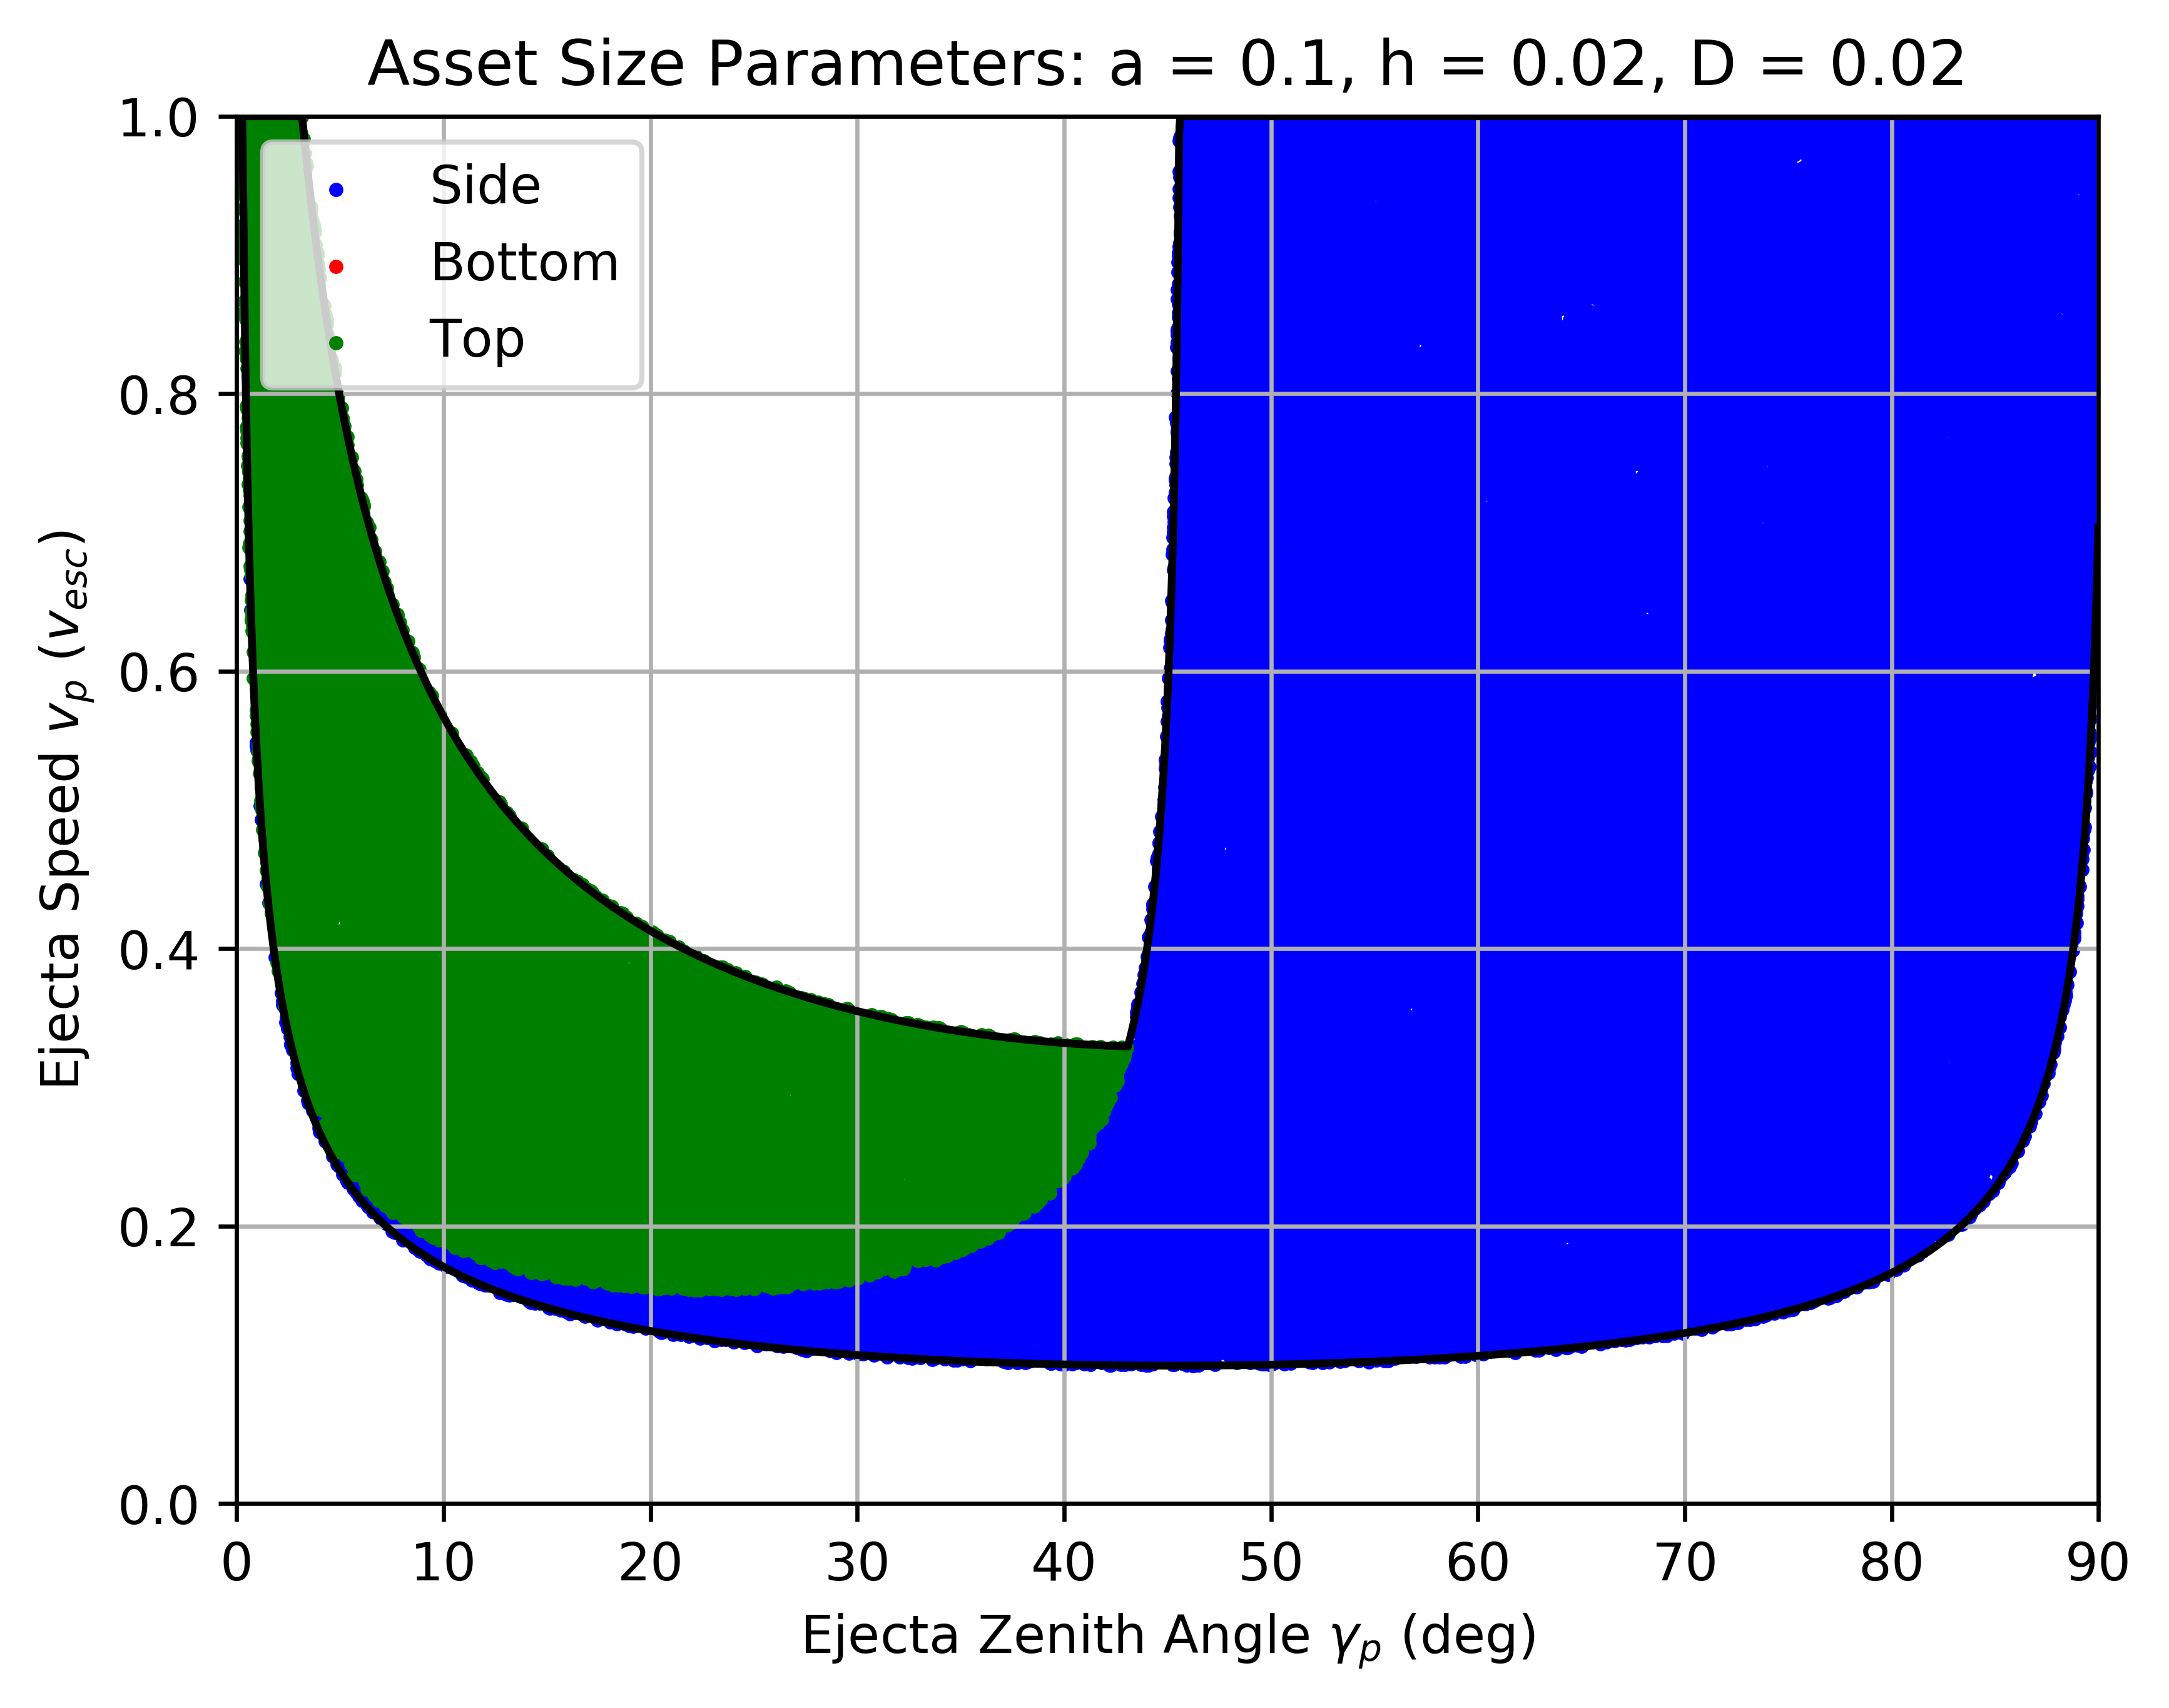
\includegraphics[width=.98\linewidth]{asset_speed_zenith_plot_1.000e-01_2.000e-02_2.000e-02.png}  
		%\caption{Put your sub-caption here}
		\label{fig:sub-asset_speed_zenith_6}
	\end{subfigure}
	
	
	\begin{subfigure}[t]{.32\textwidth}
		\centering
		% include third image
		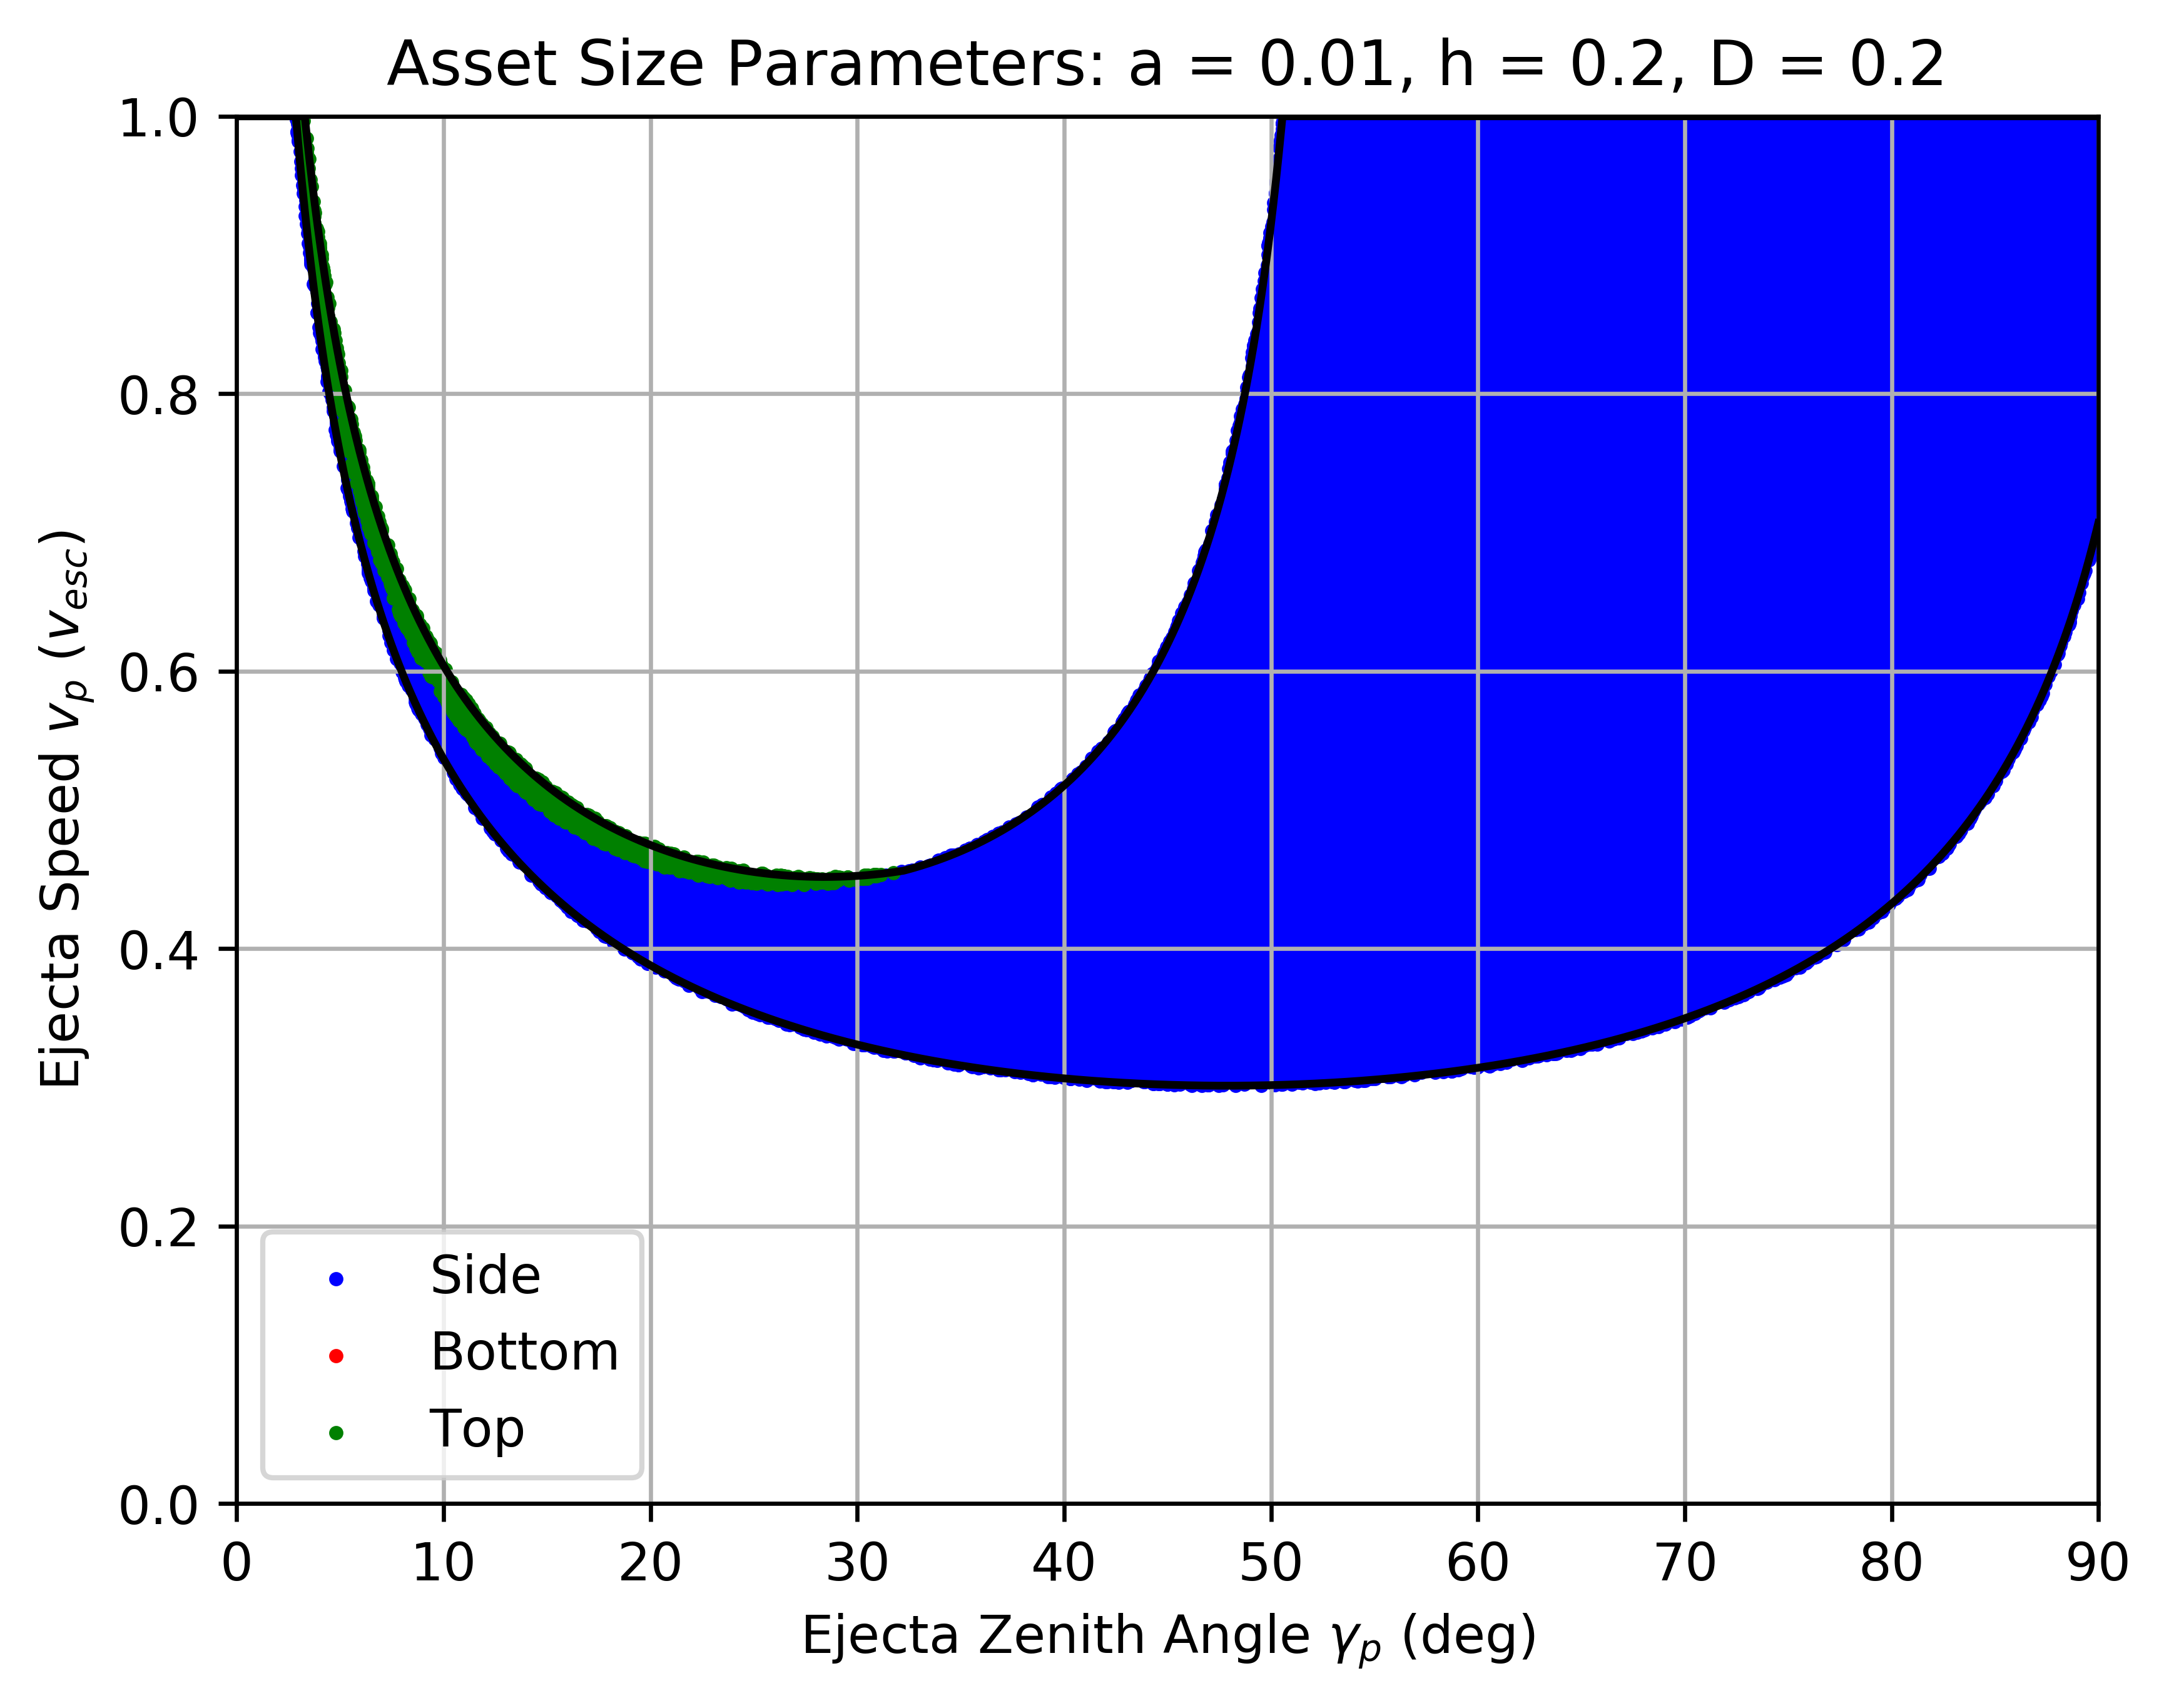
\includegraphics[width=.98\linewidth]{asset_speed_zenith_plot_1.000e-02_2.000e-01_2.000e-01.png}  
		%\caption{Put your sub-caption here}
		\label{fig:sub-asset_speed_zenith_7}
	\end{subfigure}
	\begin{subfigure}[t]{.32\textwidth}
		\centering
		% include fourth image
		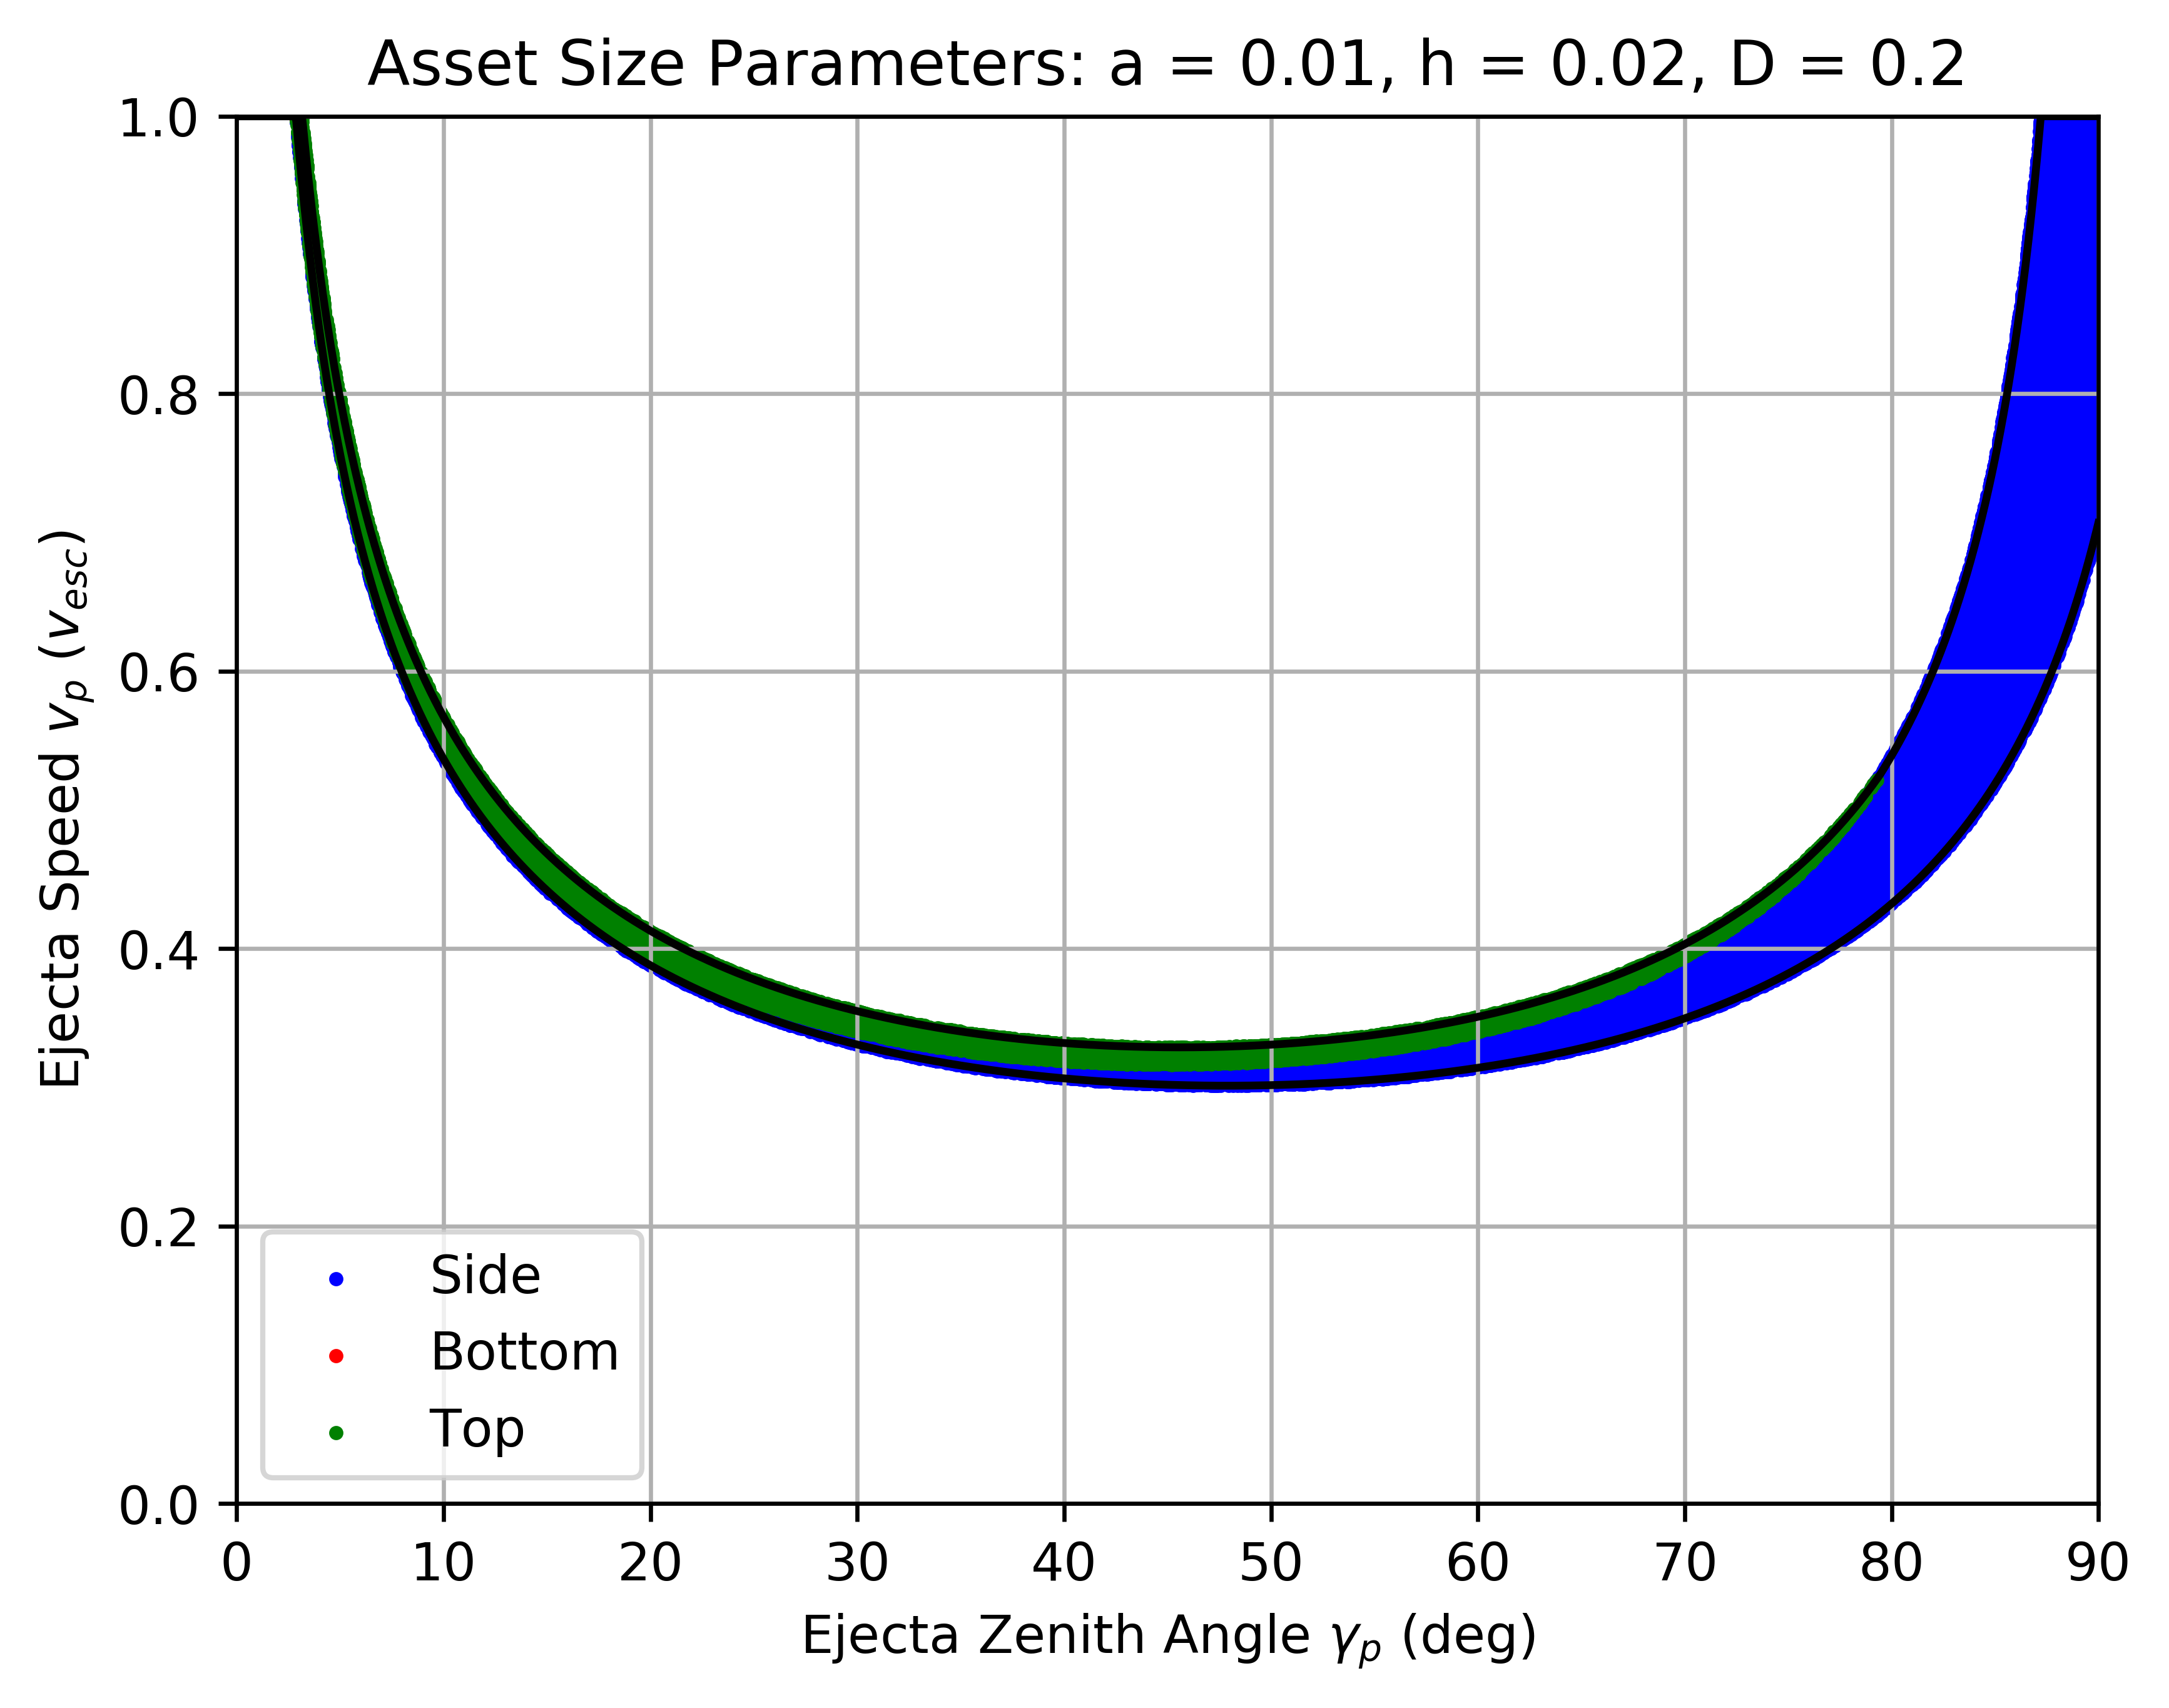
\includegraphics[width=.98\linewidth]{asset_speed_zenith_plot_1.000e-02_2.000e-02_2.000e-01.png}  
		%\caption{Put your sub-caption here}
		\label{fig:sub-asset_speed_zenith_8}
	\end{subfigure}
	\begin{subfigure}[t]{.32\textwidth}
		\centering
		% include fourth image
		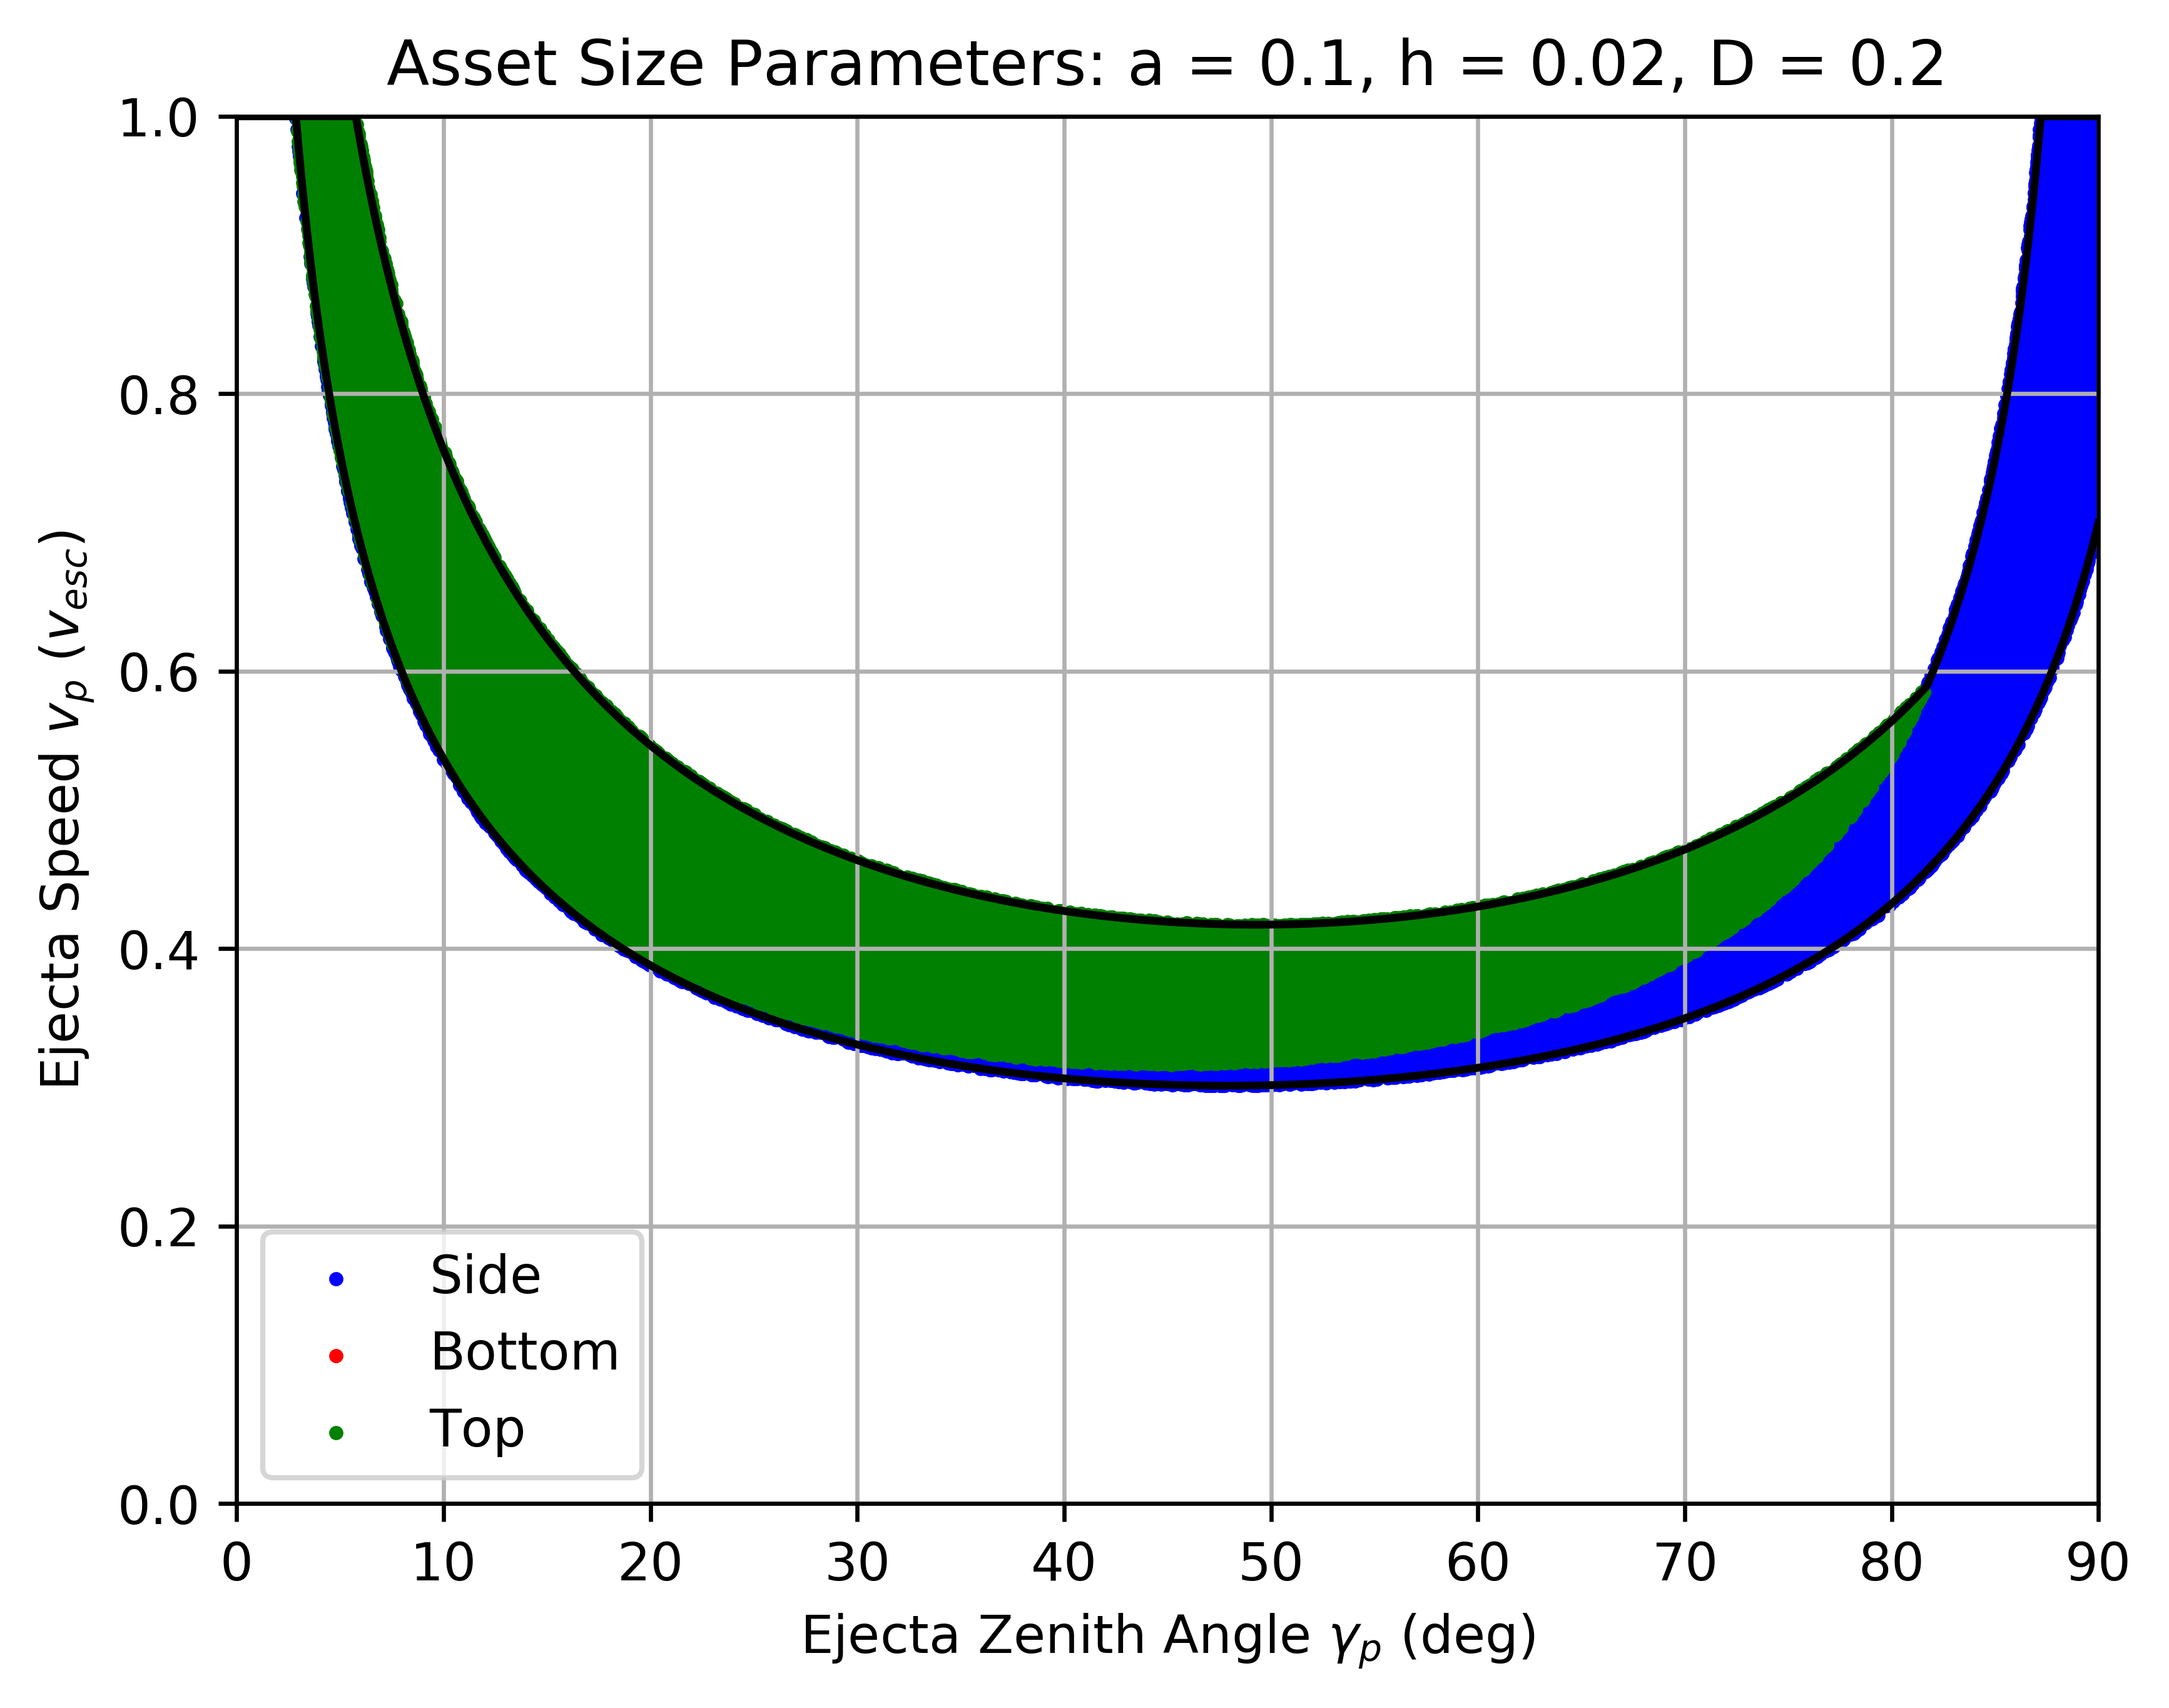
\includegraphics[width=.98\linewidth]{asset_speed_zenith_plot_1.000e-01_2.000e-02_2.000e-01.png}  
		%\caption{Put your sub-caption here}
		\label{fig:sub-asset_speed_zenith_9}
	\end{subfigure}
	
	\begin{subfigure}[t]{.32\textwidth}
		\centering
		% include third image
		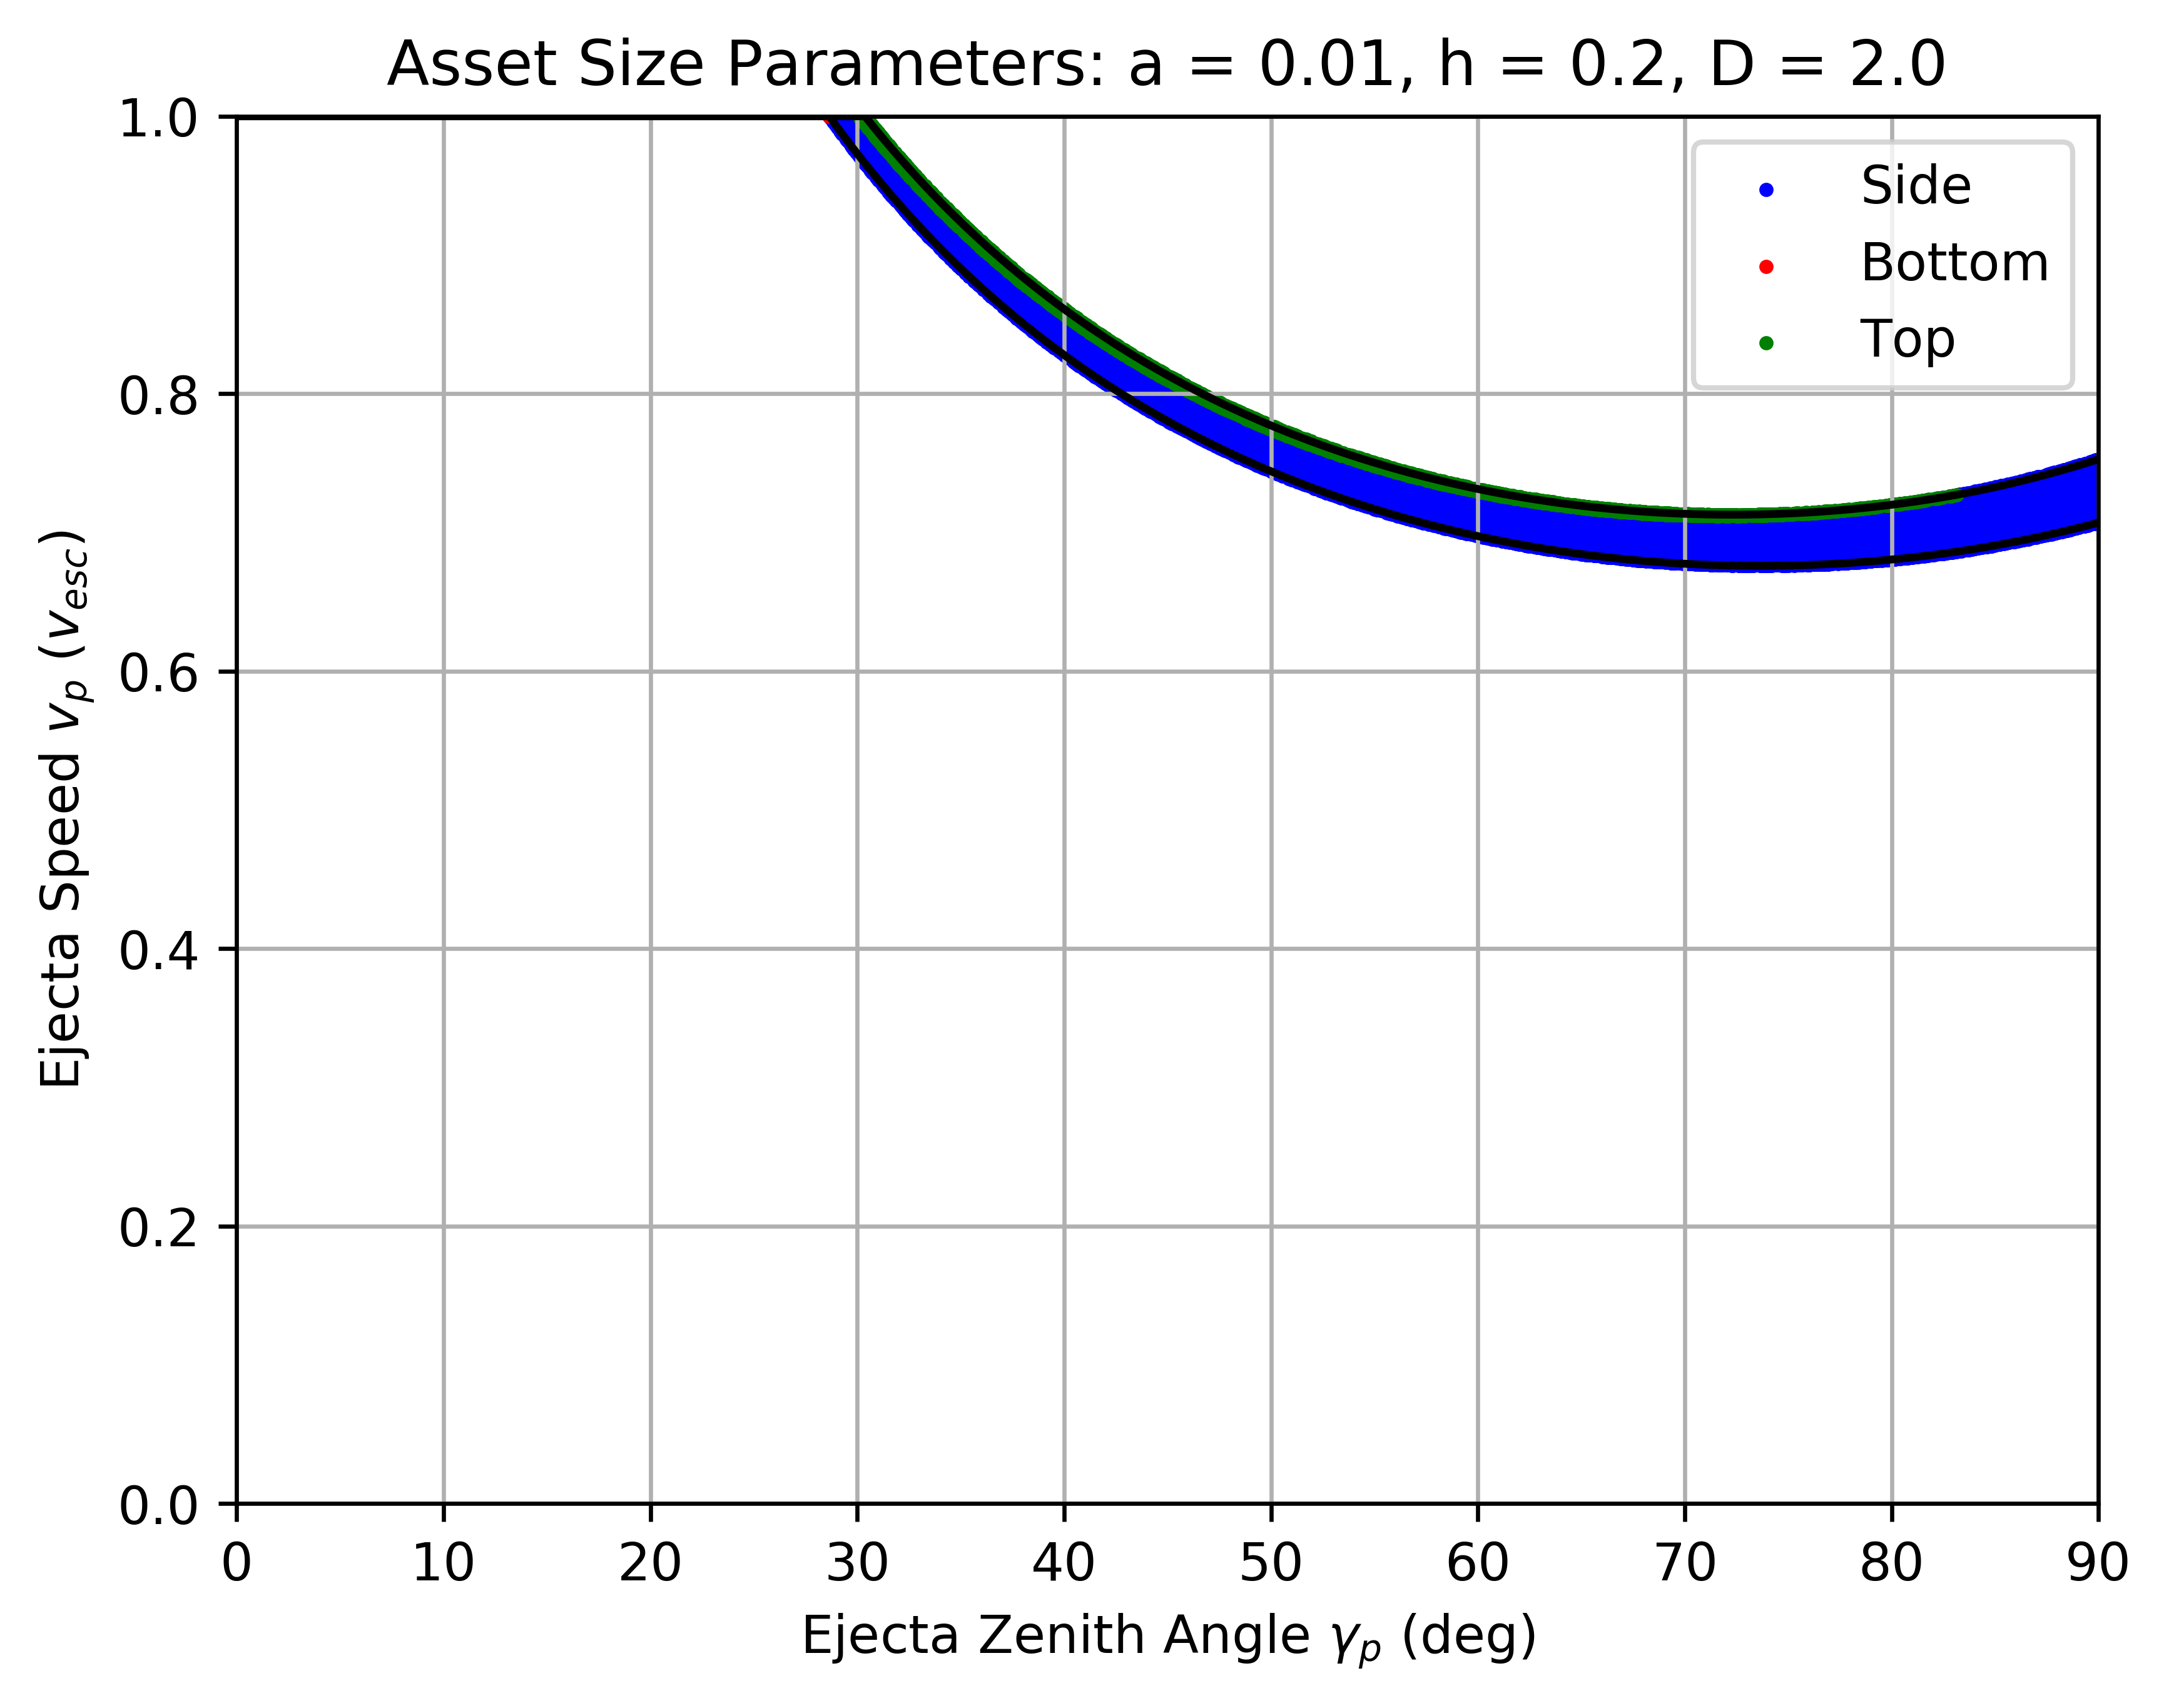
\includegraphics[width=.98\linewidth]{asset_speed_zenith_plot_1.000e-02_2.000e-01_2.000e+00.png}  
		%\caption{Put your sub-caption here}
		\label{fig:sub-asset_speed_zenith_10}
	\end{subfigure}
	\begin{subfigure}[t]{.32\textwidth}
		\centering
		% include fourth image
		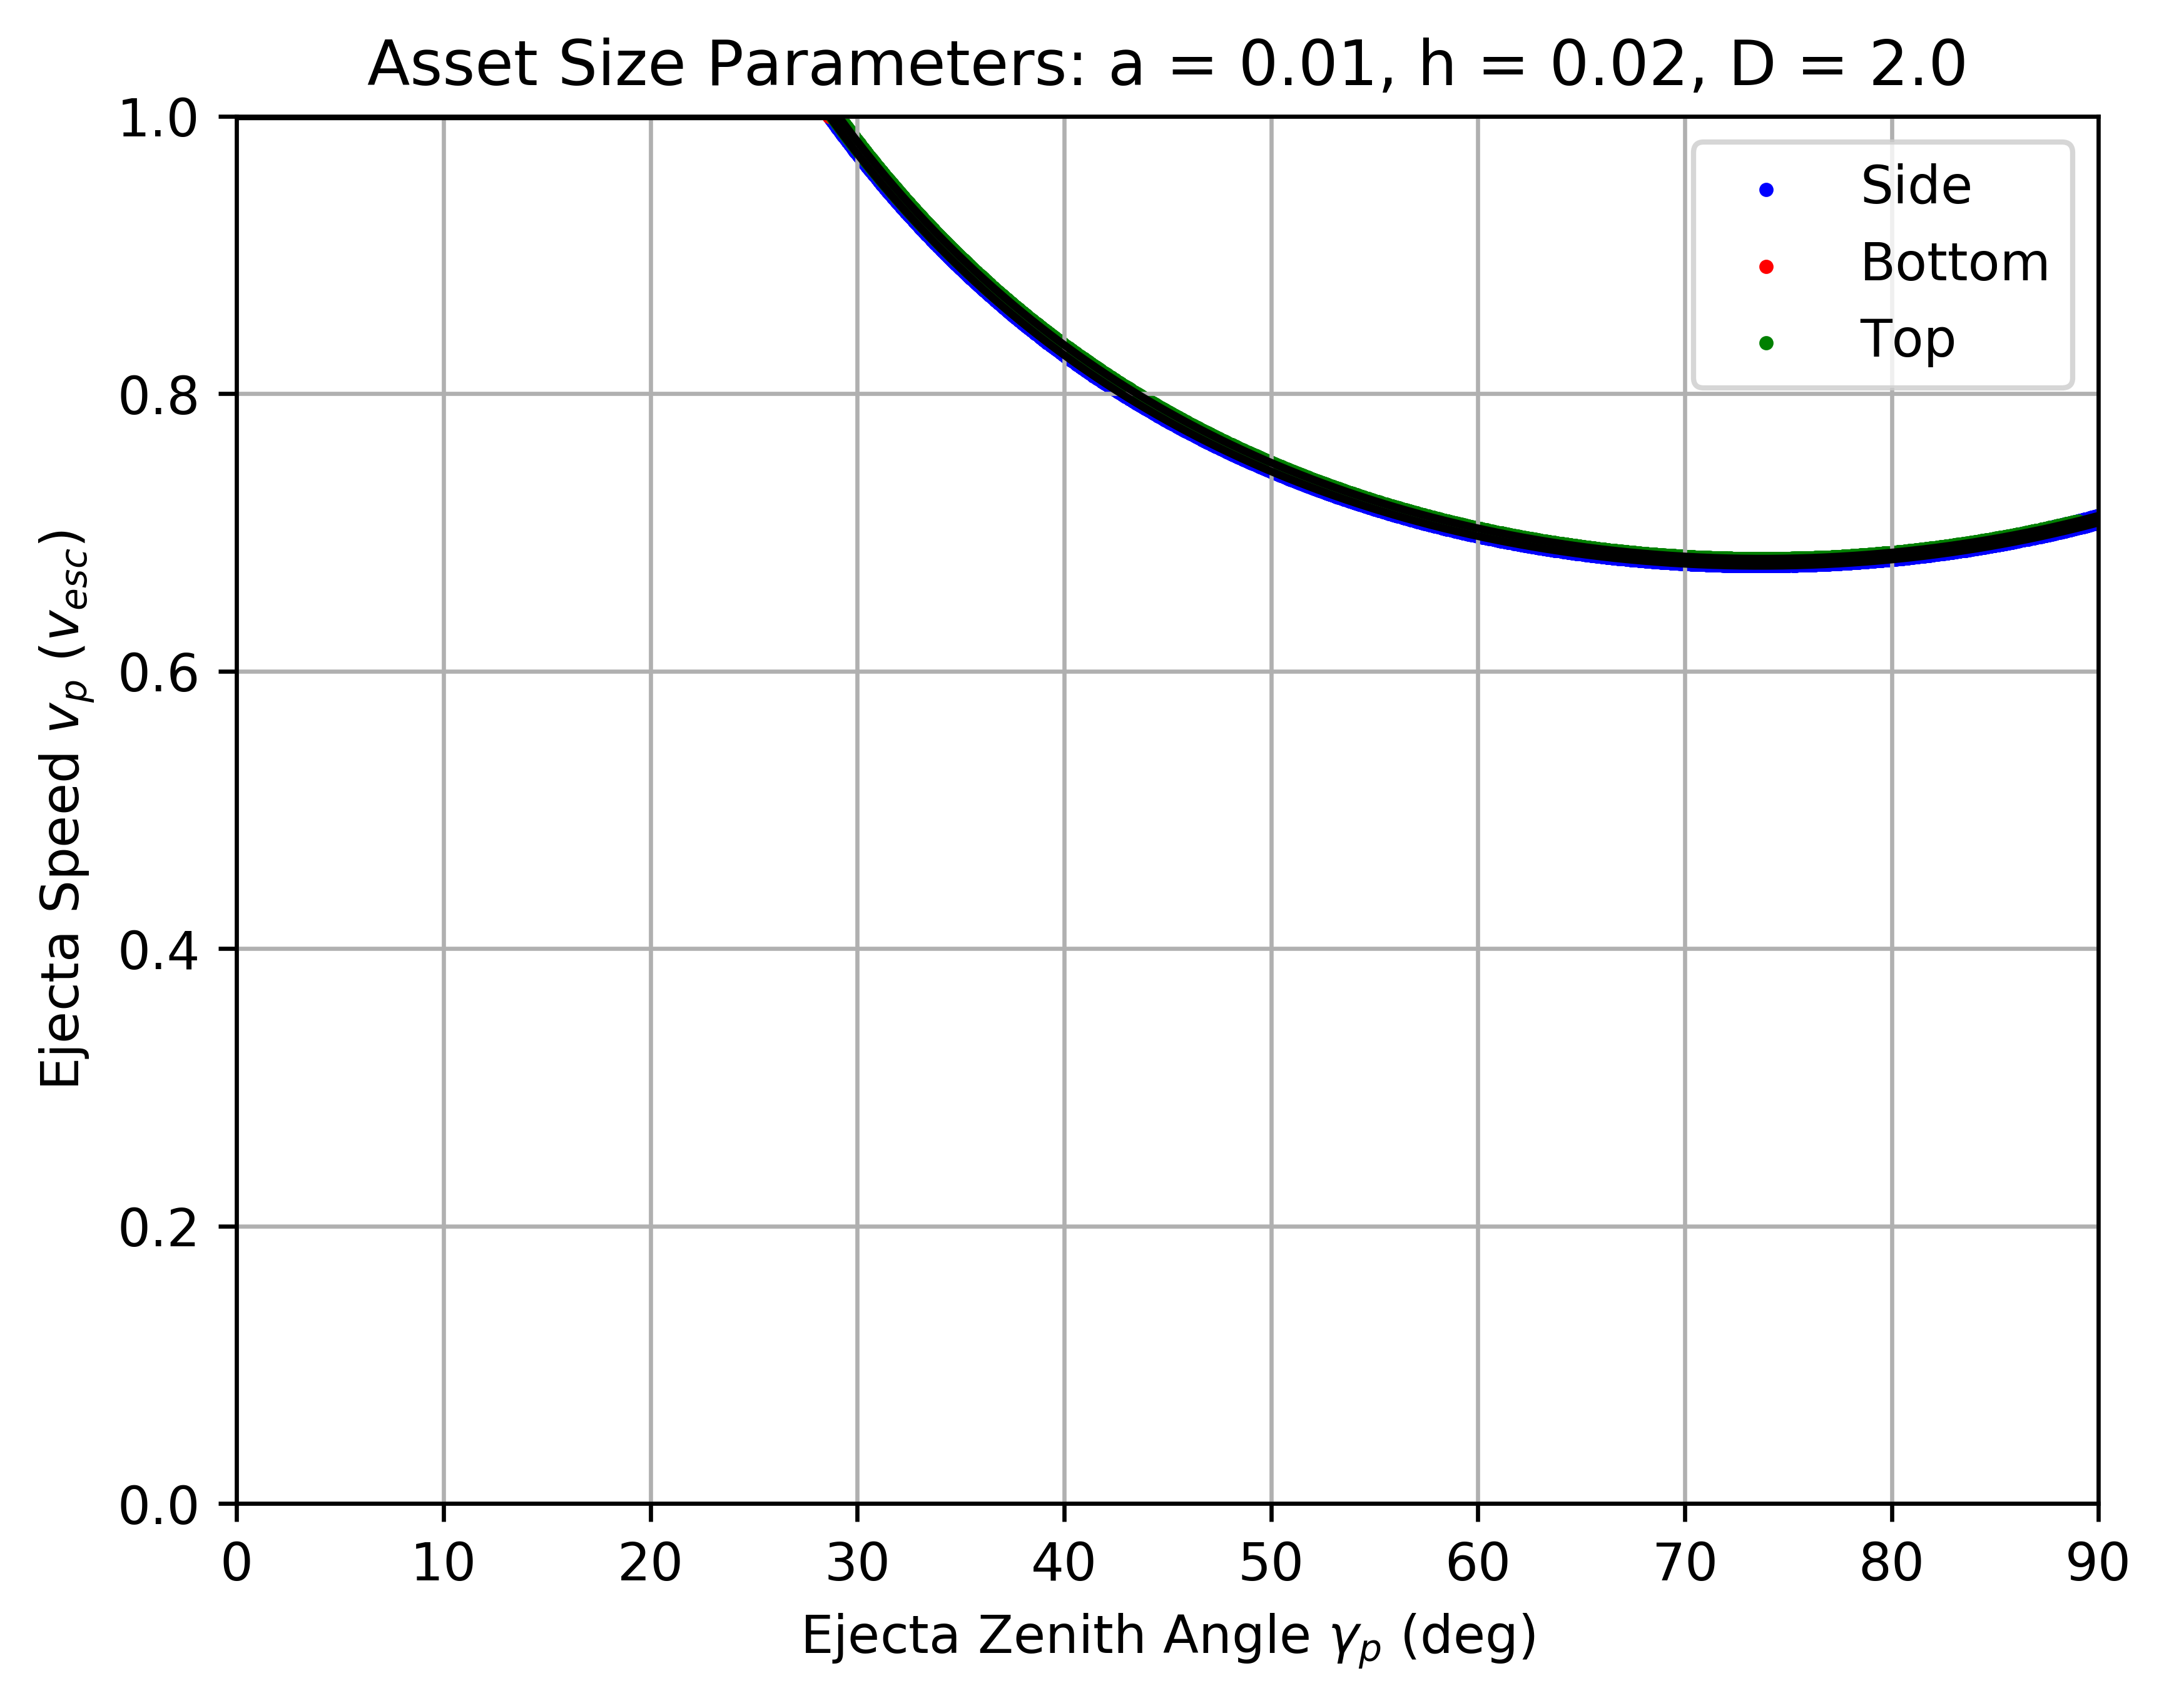
\includegraphics[width=.98\linewidth]{asset_speed_zenith_plot_1.000e-02_2.000e-02_2.000e+00.png}  
		%\caption{Put your sub-caption here}
		\label{fig:sub-asset_speed_zenith_11}
	\end{subfigure}
	\begin{subfigure}[t]{.32\textwidth}
		\centering
		% include fourth image
		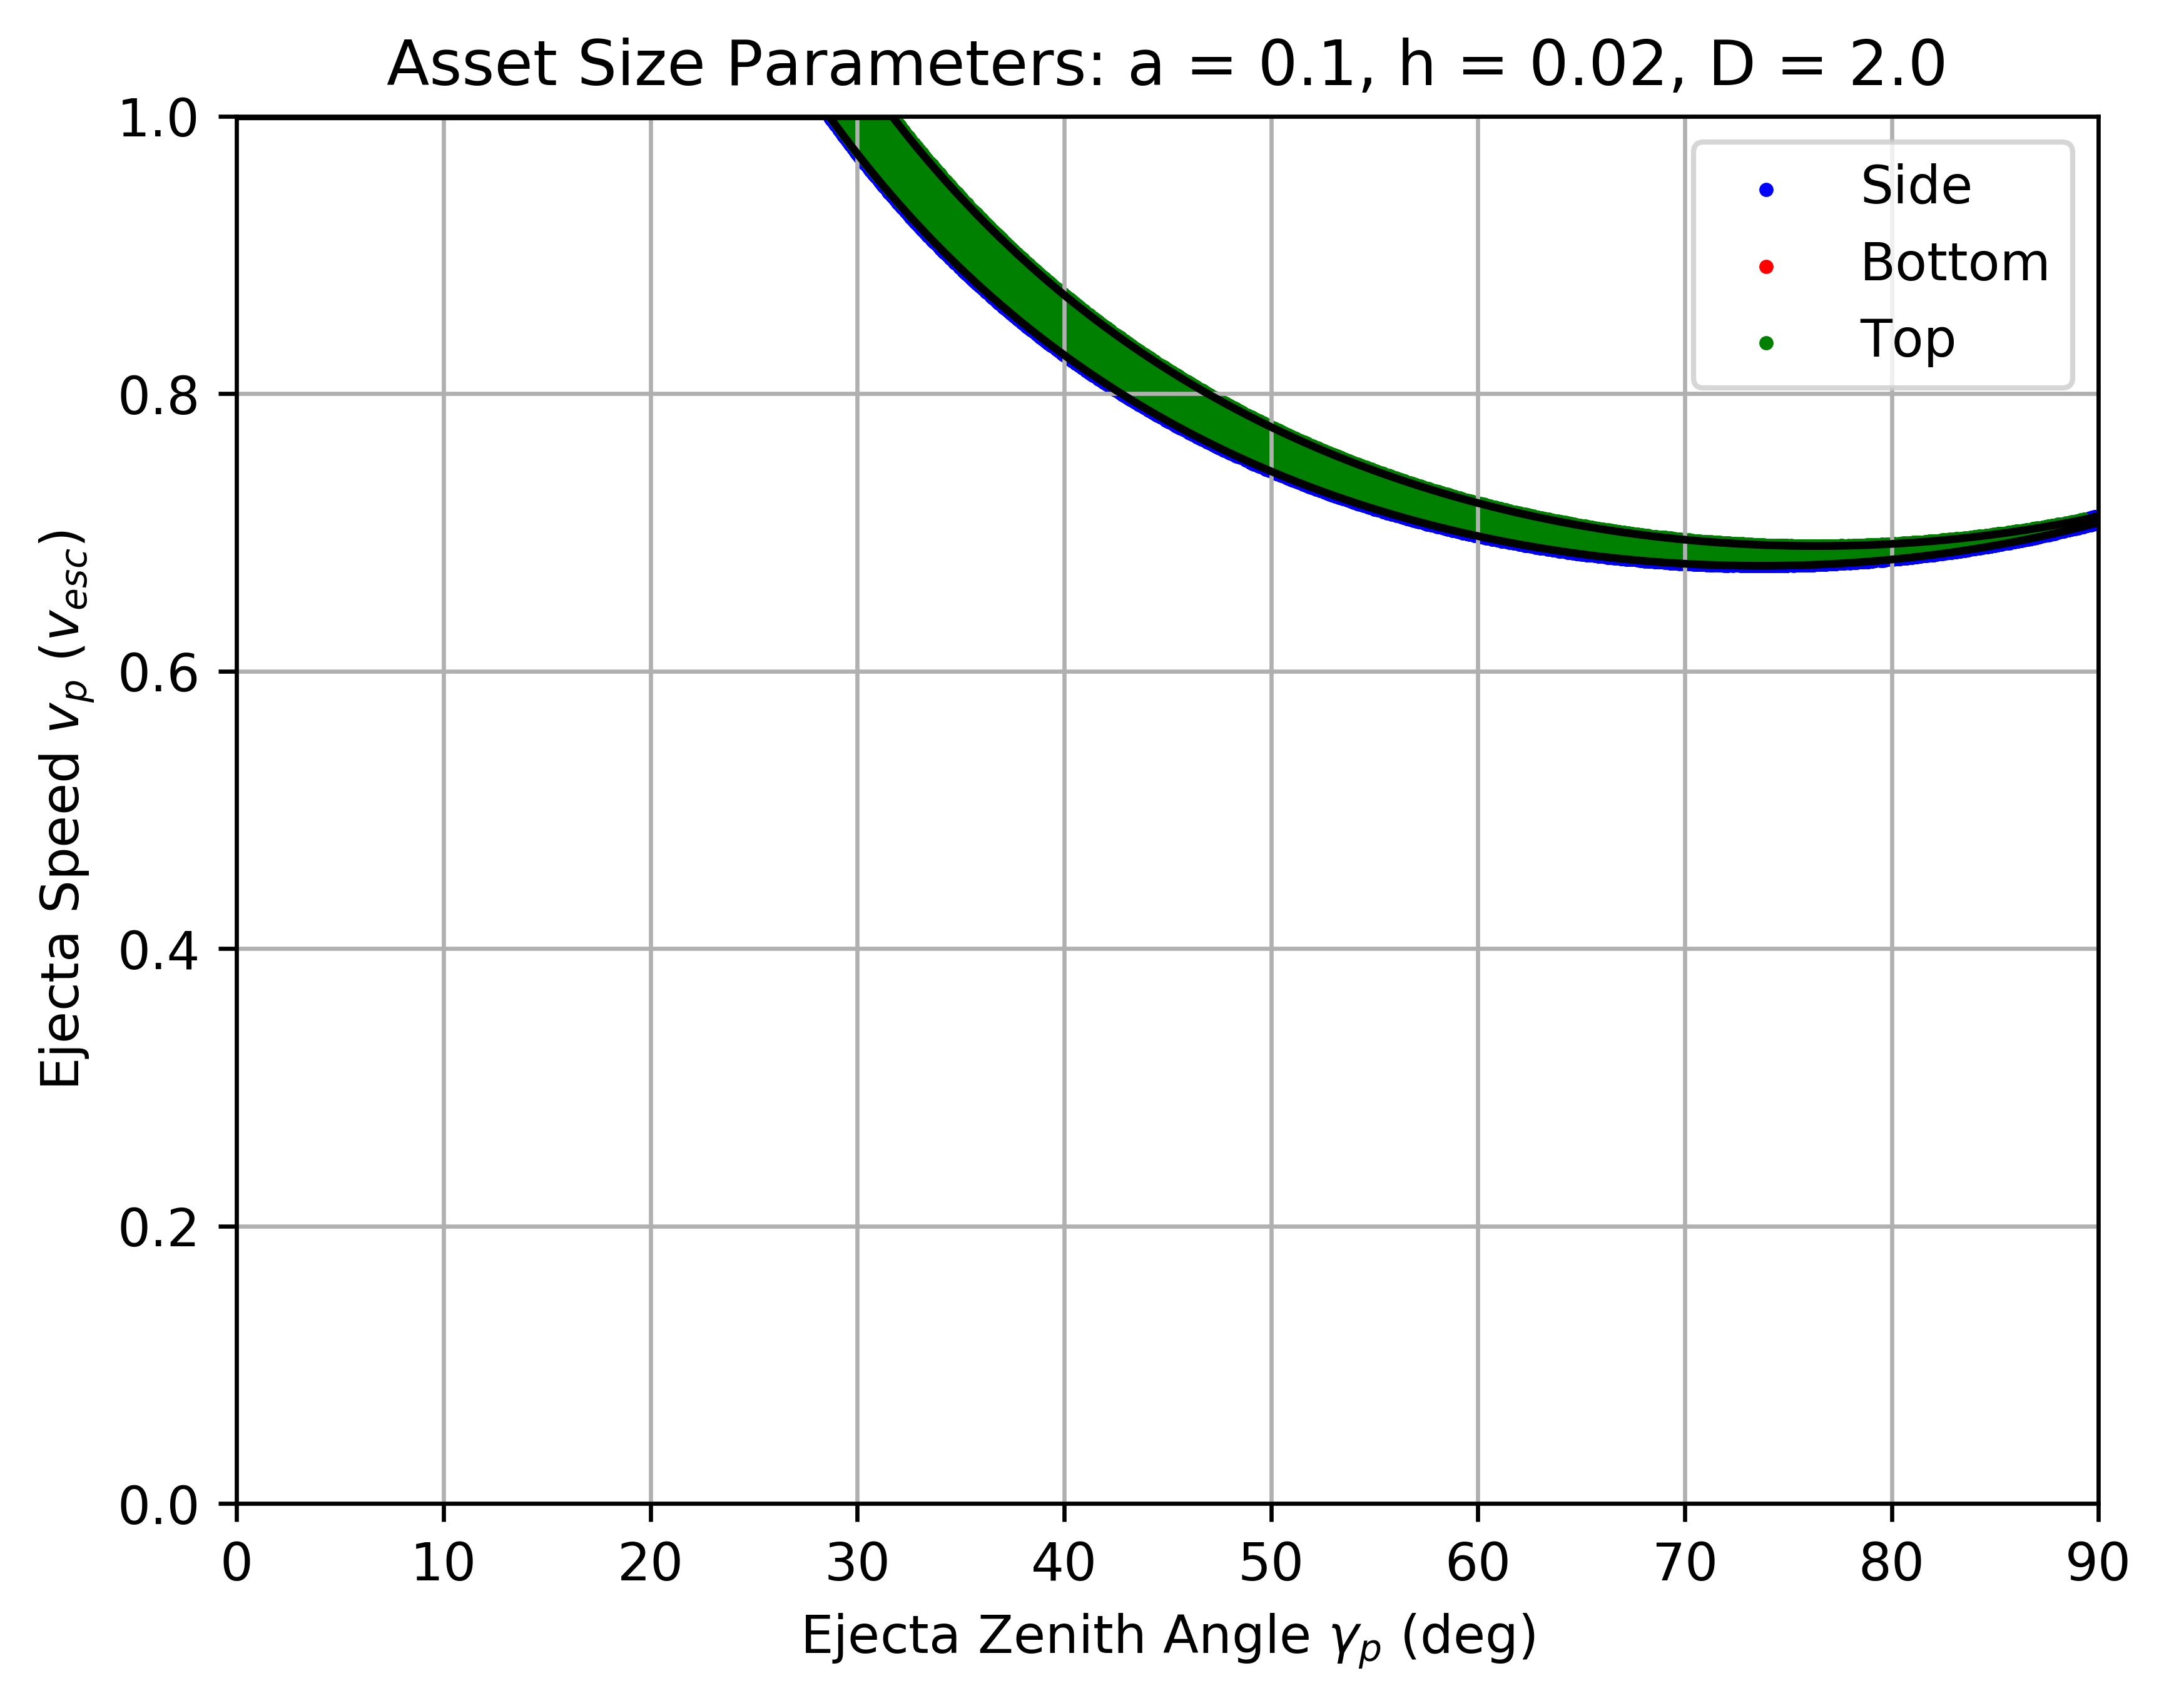
\includegraphics[width=.98\linewidth]{asset_speed_zenith_plot_1.000e-01_2.000e-02_2.000e+00.png}  
		%\caption{Put your sub-caption here}
		\label{fig:sub-asset_speed_zenith_12}
	\end{subfigure}
	
	\caption{A matrix of plots showing the ejecta hitting a cylindrical asset (in a plane intersecting the cylinder's symmetry axis) on the surface for various asset sizes and crater-to-asset distances. Each plot gives three colors for the ejecta hitting the side (blue), bottom (red), and the top (green) as a function of initial ejecta speed $v_p$ vs.\ initial ejecta zenith angle $\gamma_p$.}
	\label{fig:asset_speed_zenith_comparison}
\end{figure}









\begin{figure}
	\begin{subfigure}[t]{.32\textwidth}
		\centering
		% include first image
		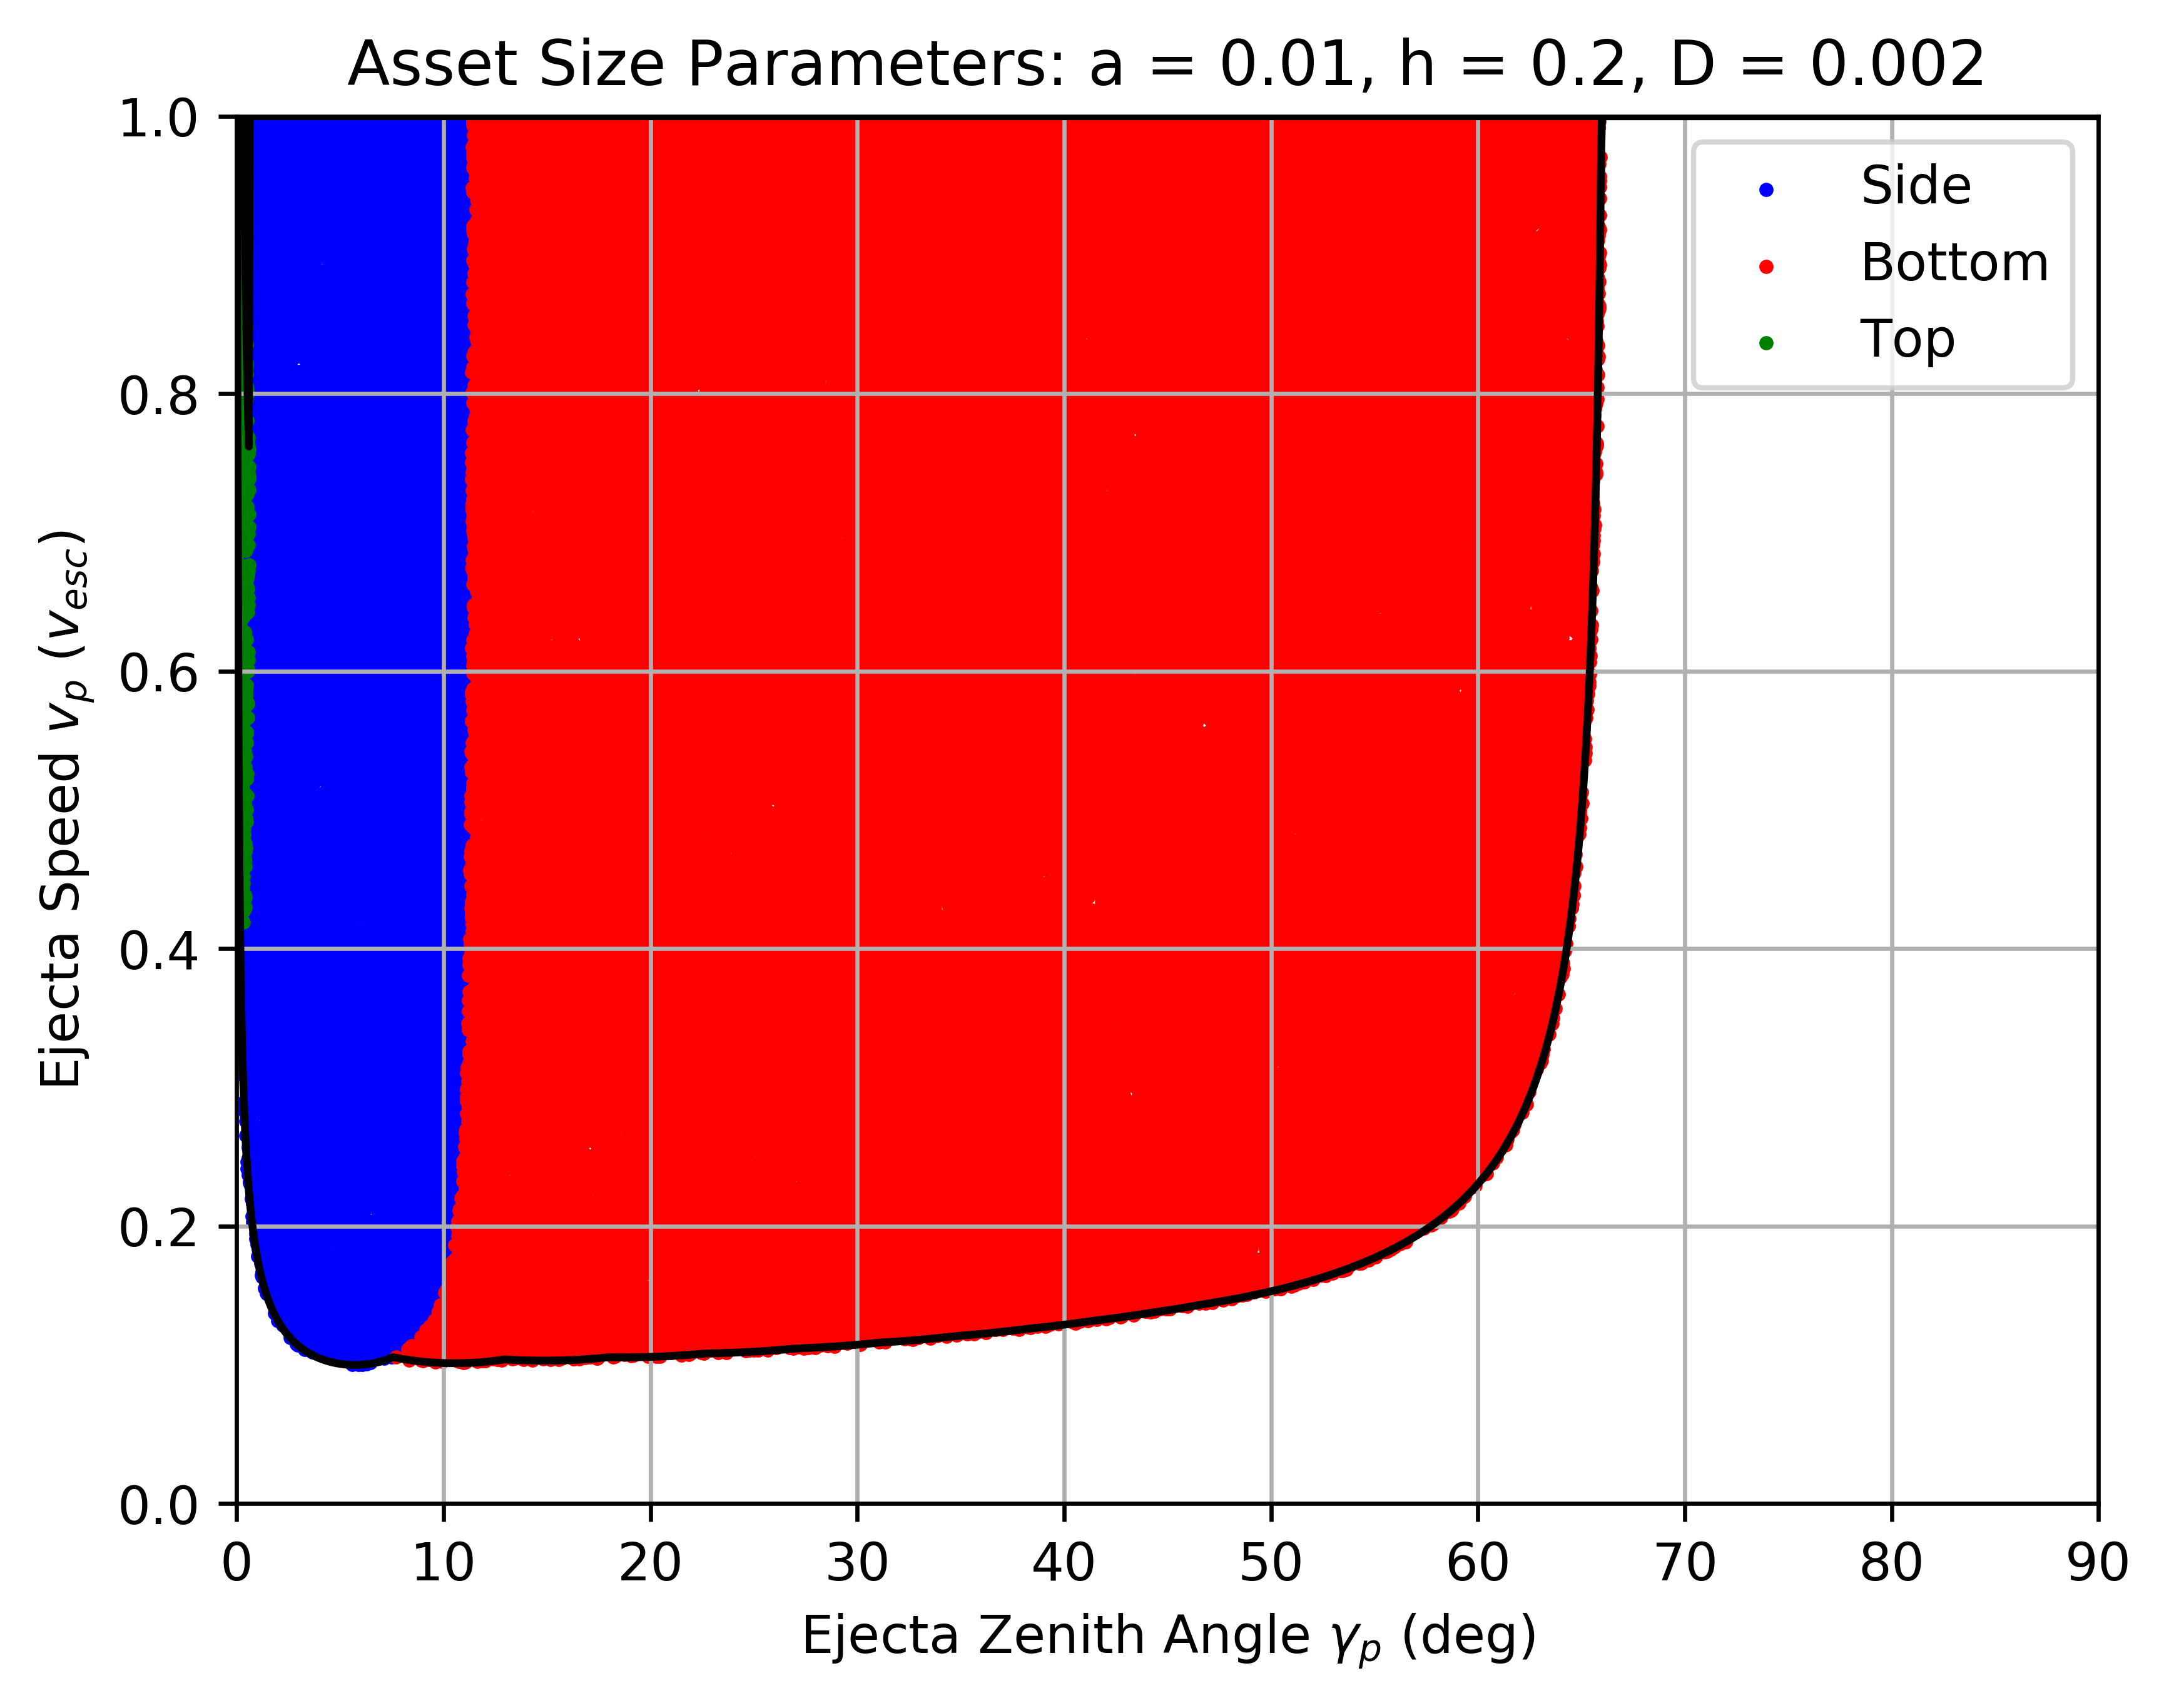
\includegraphics[width=.98\linewidth]{asset_speed_zenith_plot_1.010e+00_1.000e-02_2.000e-01_2.000e-03.png}  
		%\caption{Put your sub-caption here}
		\label{fig:sub-asset_speed_zenith_h1_1}
	\end{subfigure}
	\begin{subfigure}[t]{.32\textwidth}
		\centering
		% include second image
		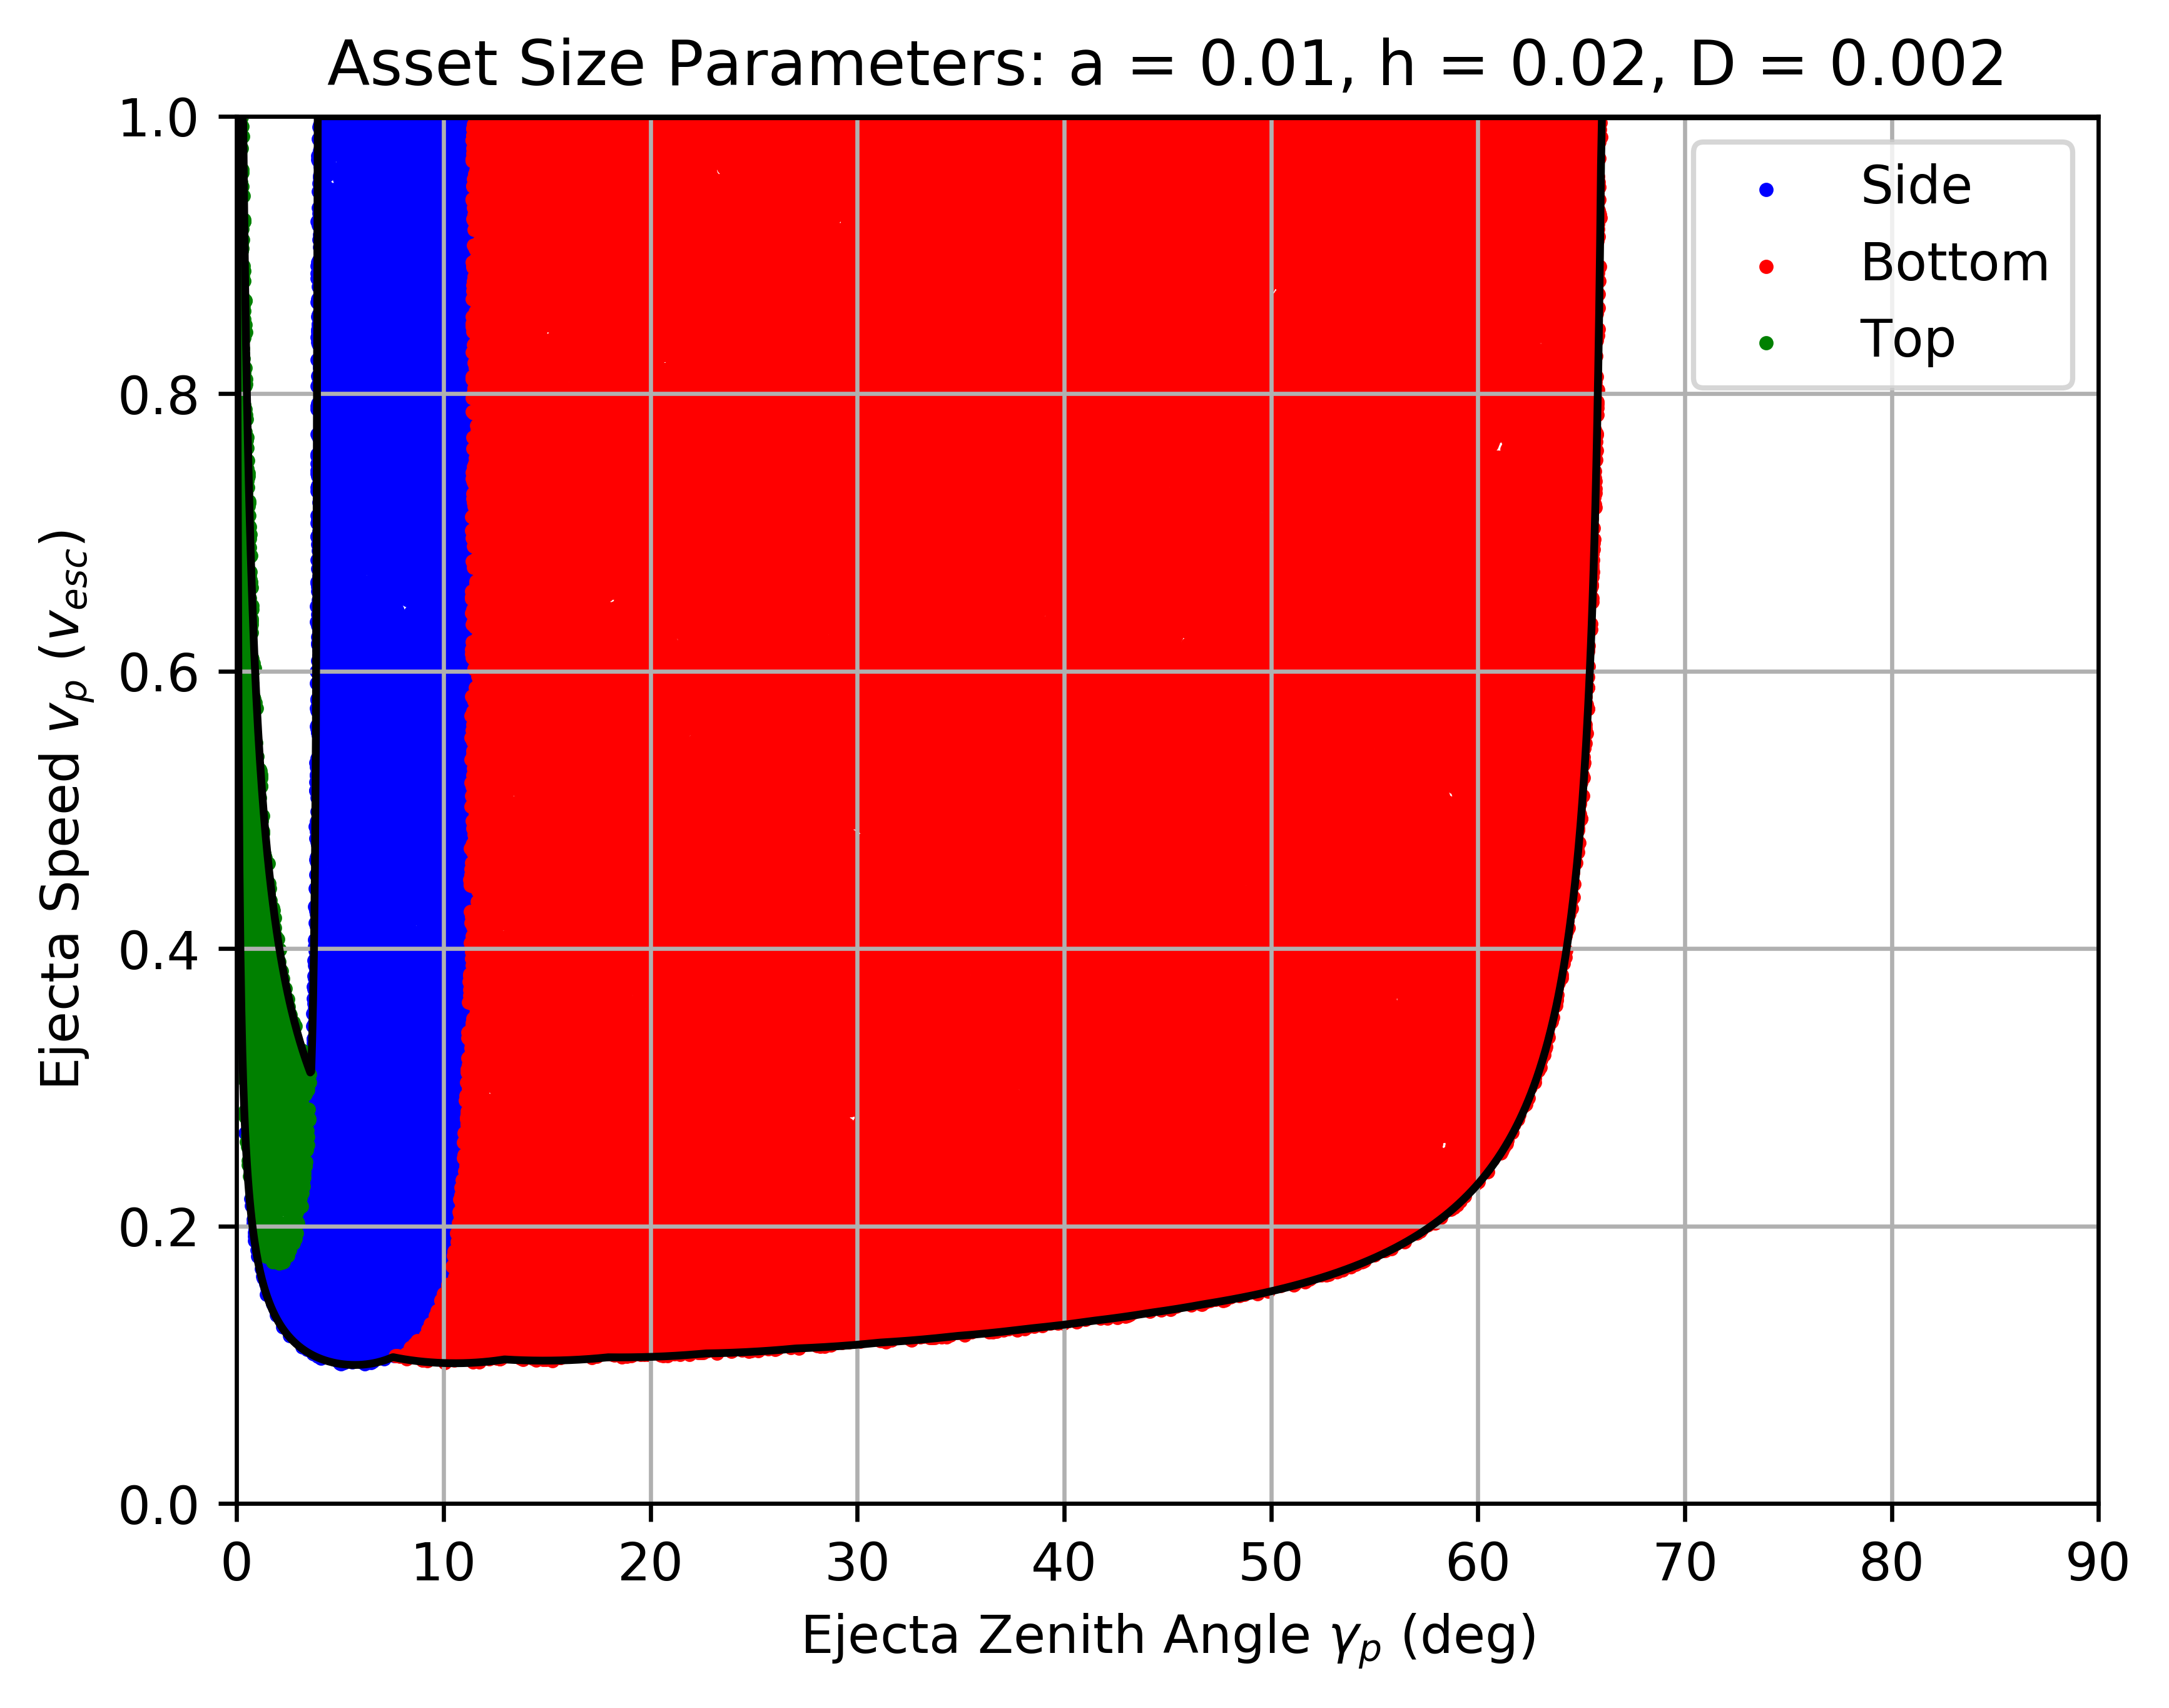
\includegraphics[width=.98\linewidth]{asset_speed_zenith_plot_1.010e+00_1.000e-02_2.000e-02_2.000e-03.png}  
		%\caption{Put your sub-caption here}
		\label{fig:sub-asset_speed_zenith_h1_2}
	\end{subfigure}
	\begin{subfigure}[t]{.32\textwidth}
		\centering
		% include second image
		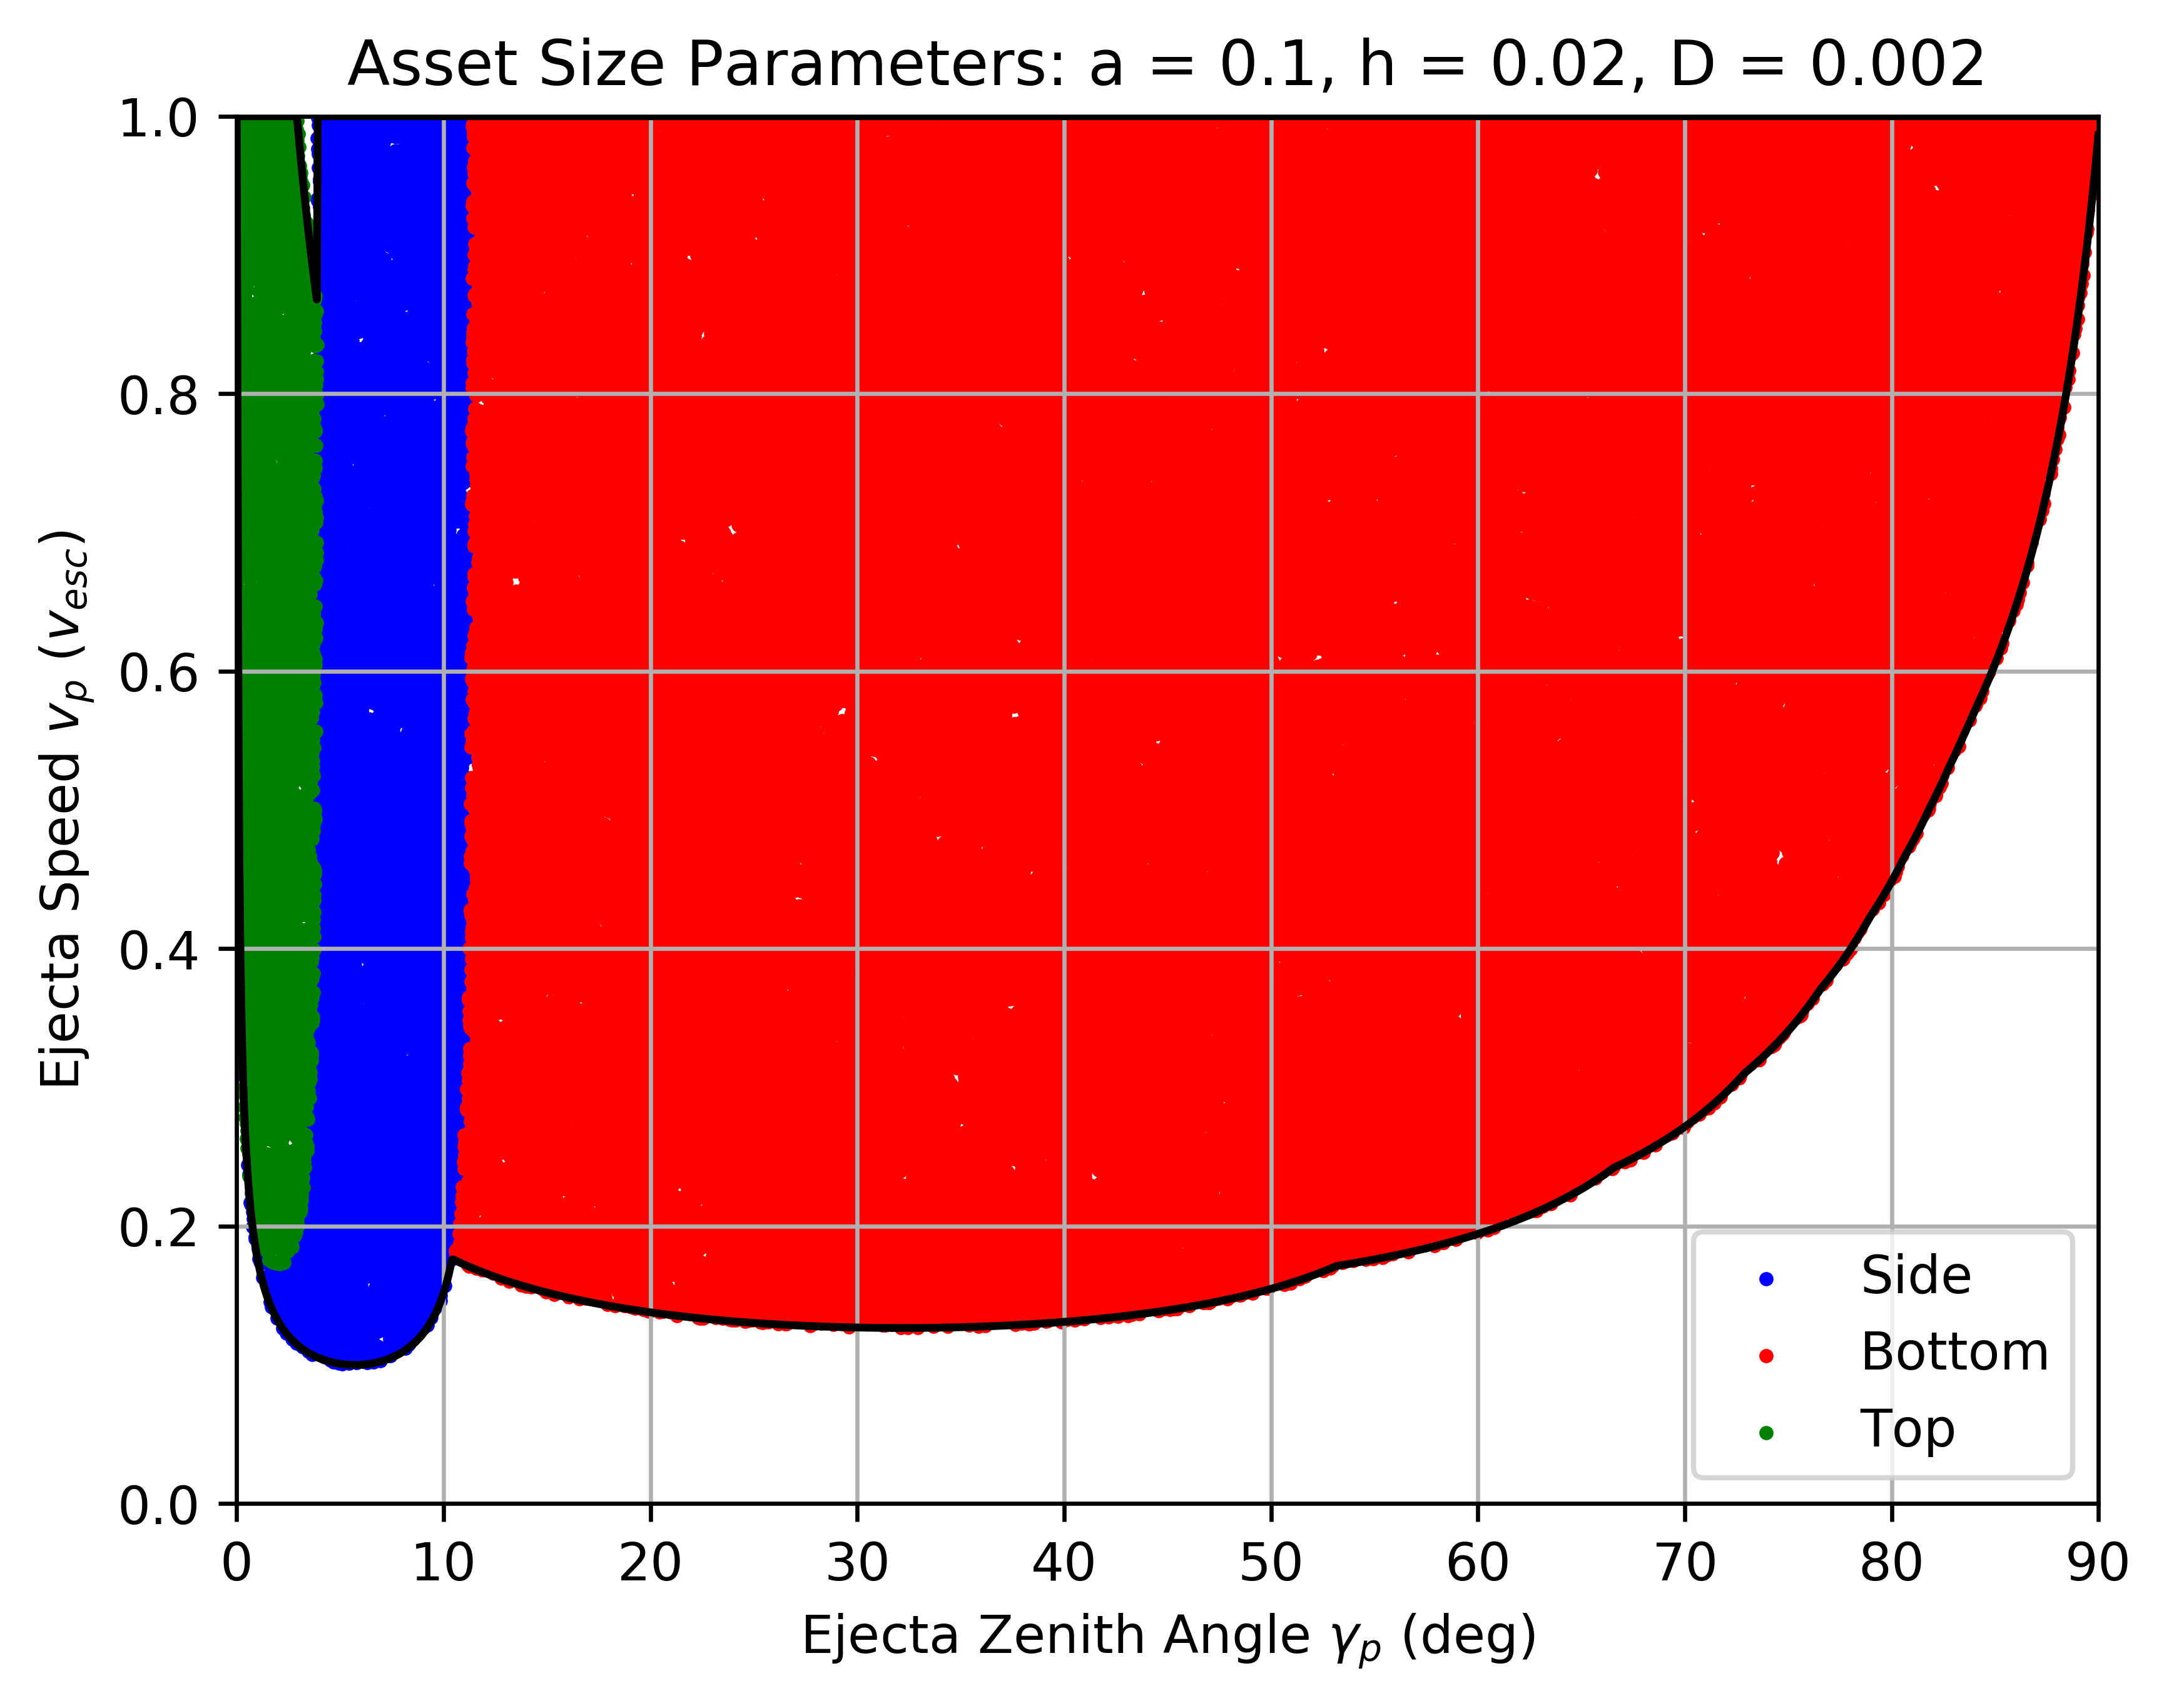
\includegraphics[width=.98\linewidth]{asset_speed_zenith_plot_1.010e+00_1.000e-01_2.000e-02_2.000e-03.png}  
		%\caption{Put your sub-caption here}
		\label{fig:sub-asset_speed_zenith_h1_3}
	\end{subfigure}
	
	%\newline
	
	\begin{subfigure}[t]{.32\textwidth}
		\centering
		% include third image
		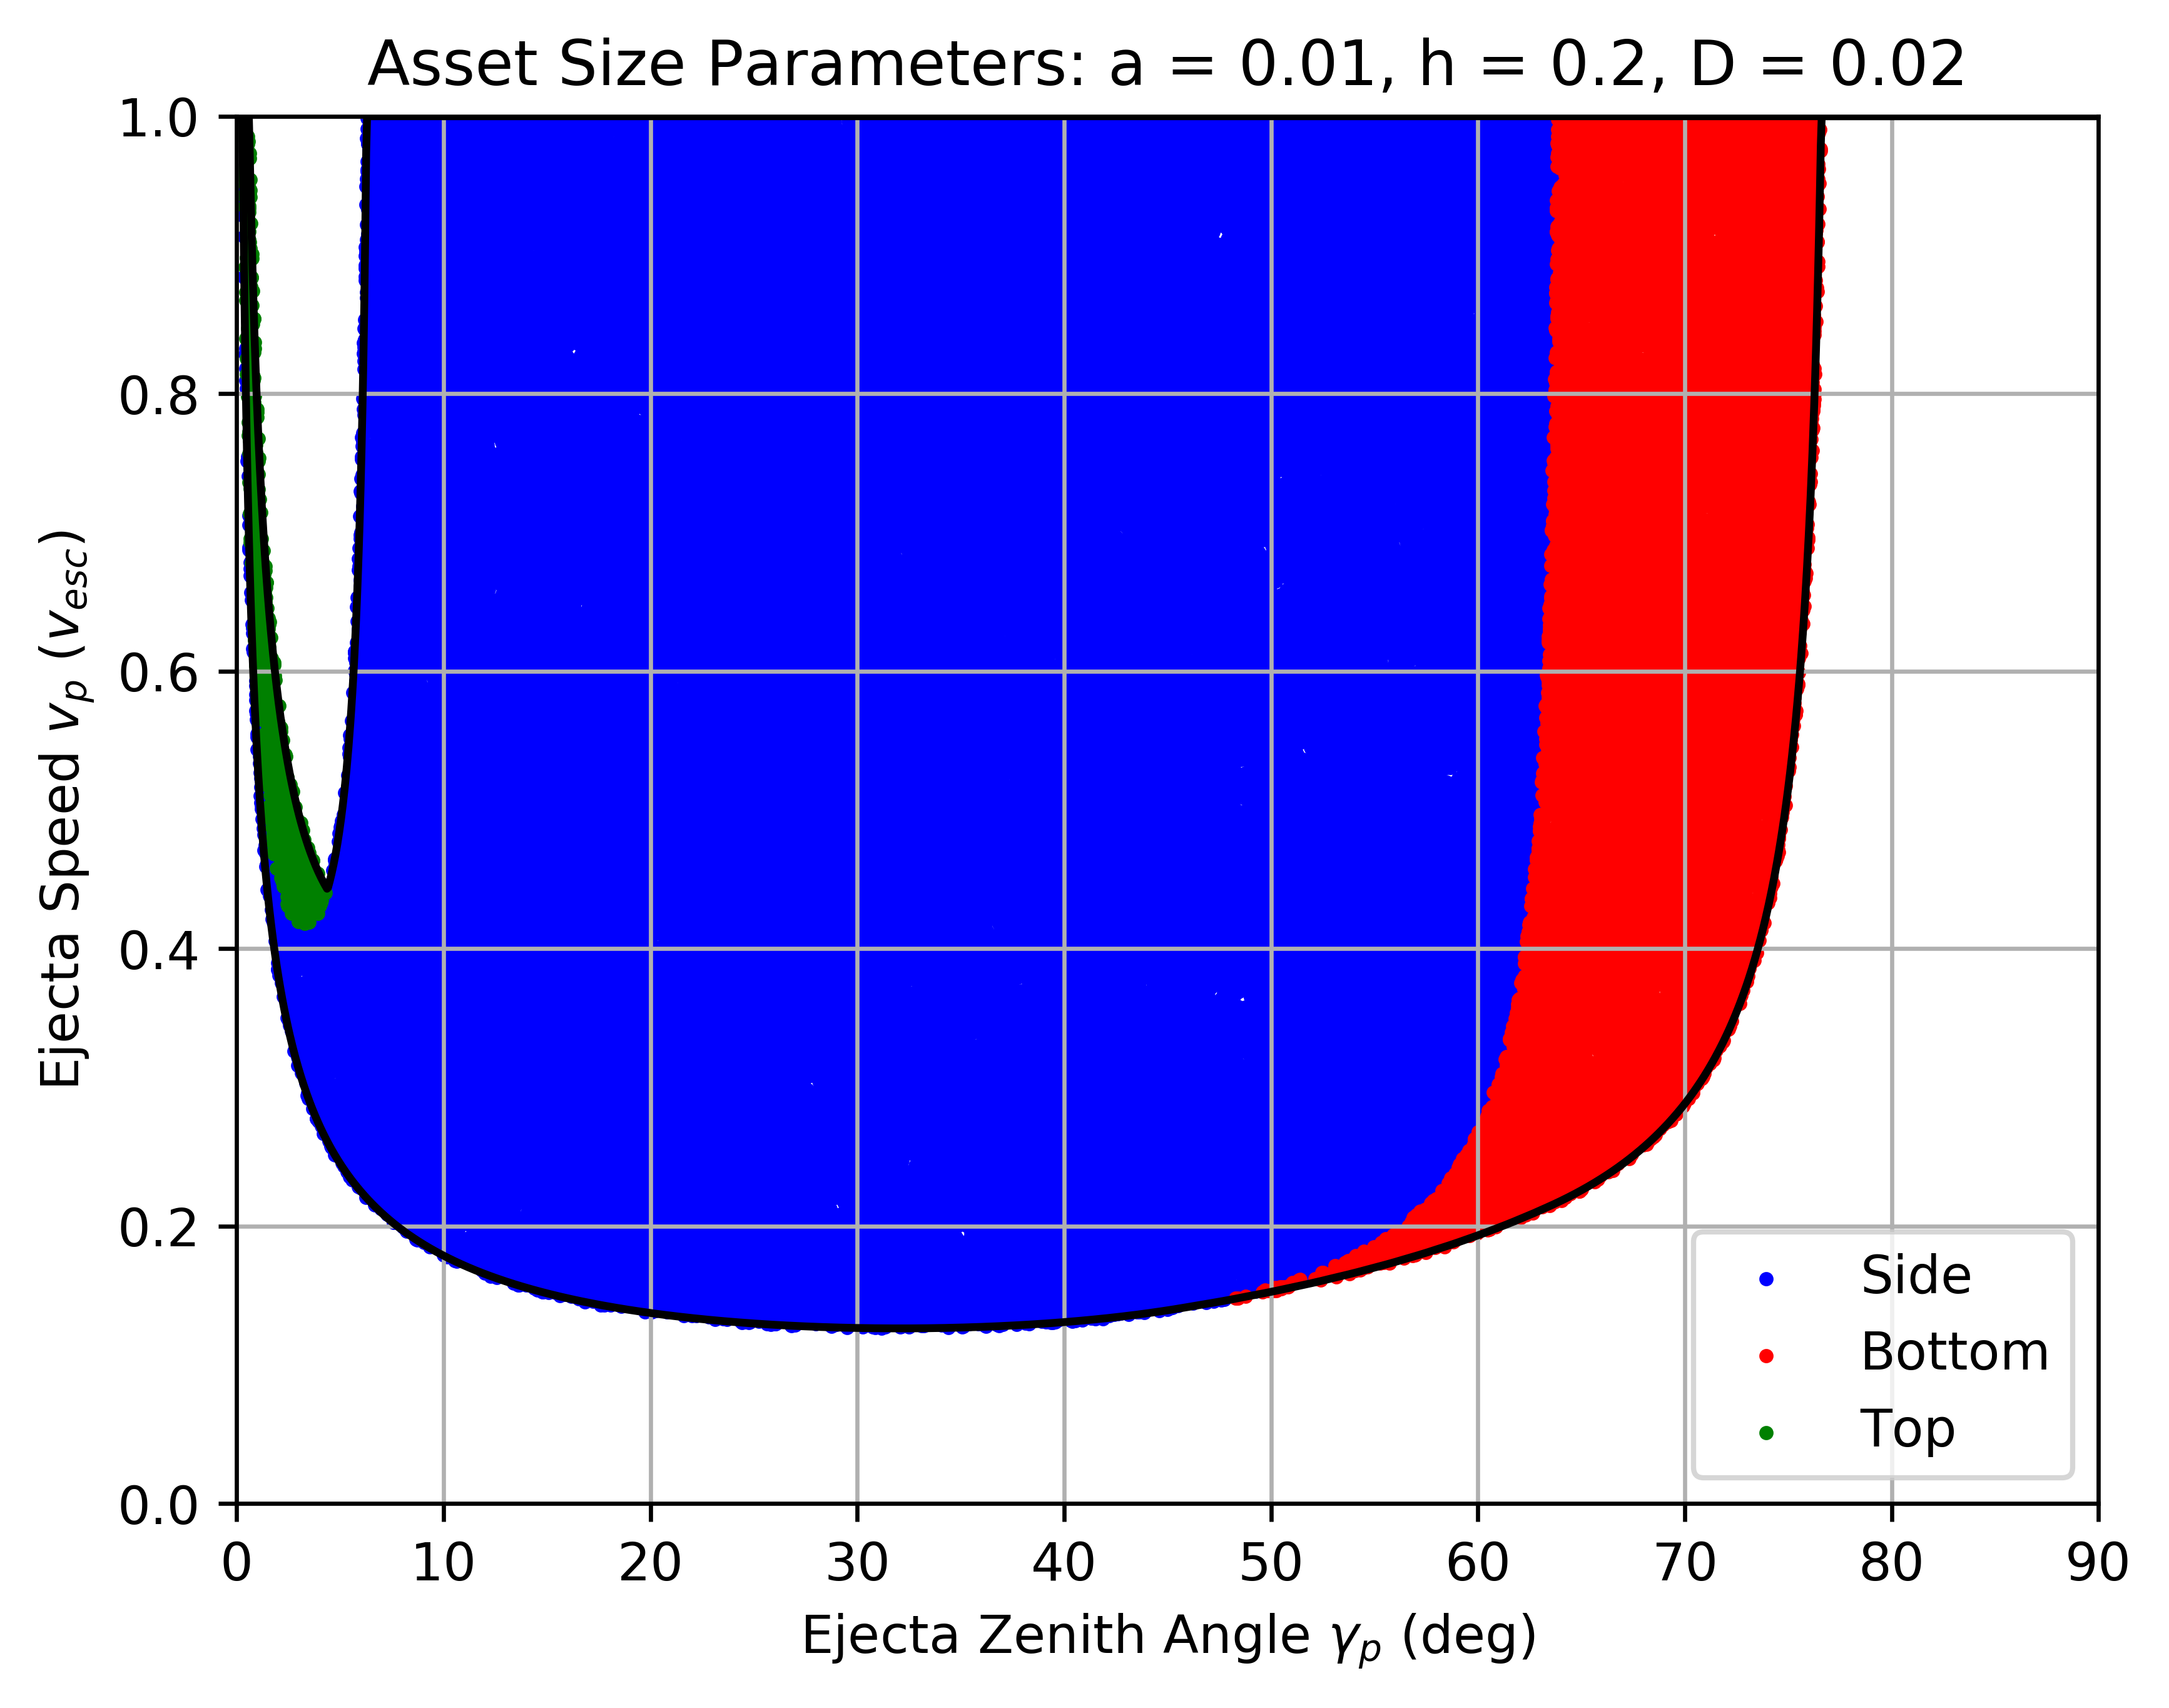
\includegraphics[width=.98\linewidth]{asset_speed_zenith_plot_1.010e+00_1.000e-02_2.000e-01_2.000e-02.png}  
		%\caption{Put your sub-caption here}
		\label{fig:sub-asset_speed_zenith_h1_4}
	\end{subfigure}
	\begin{subfigure}[t]{.32\textwidth}
		\centering
		% include fourth image
		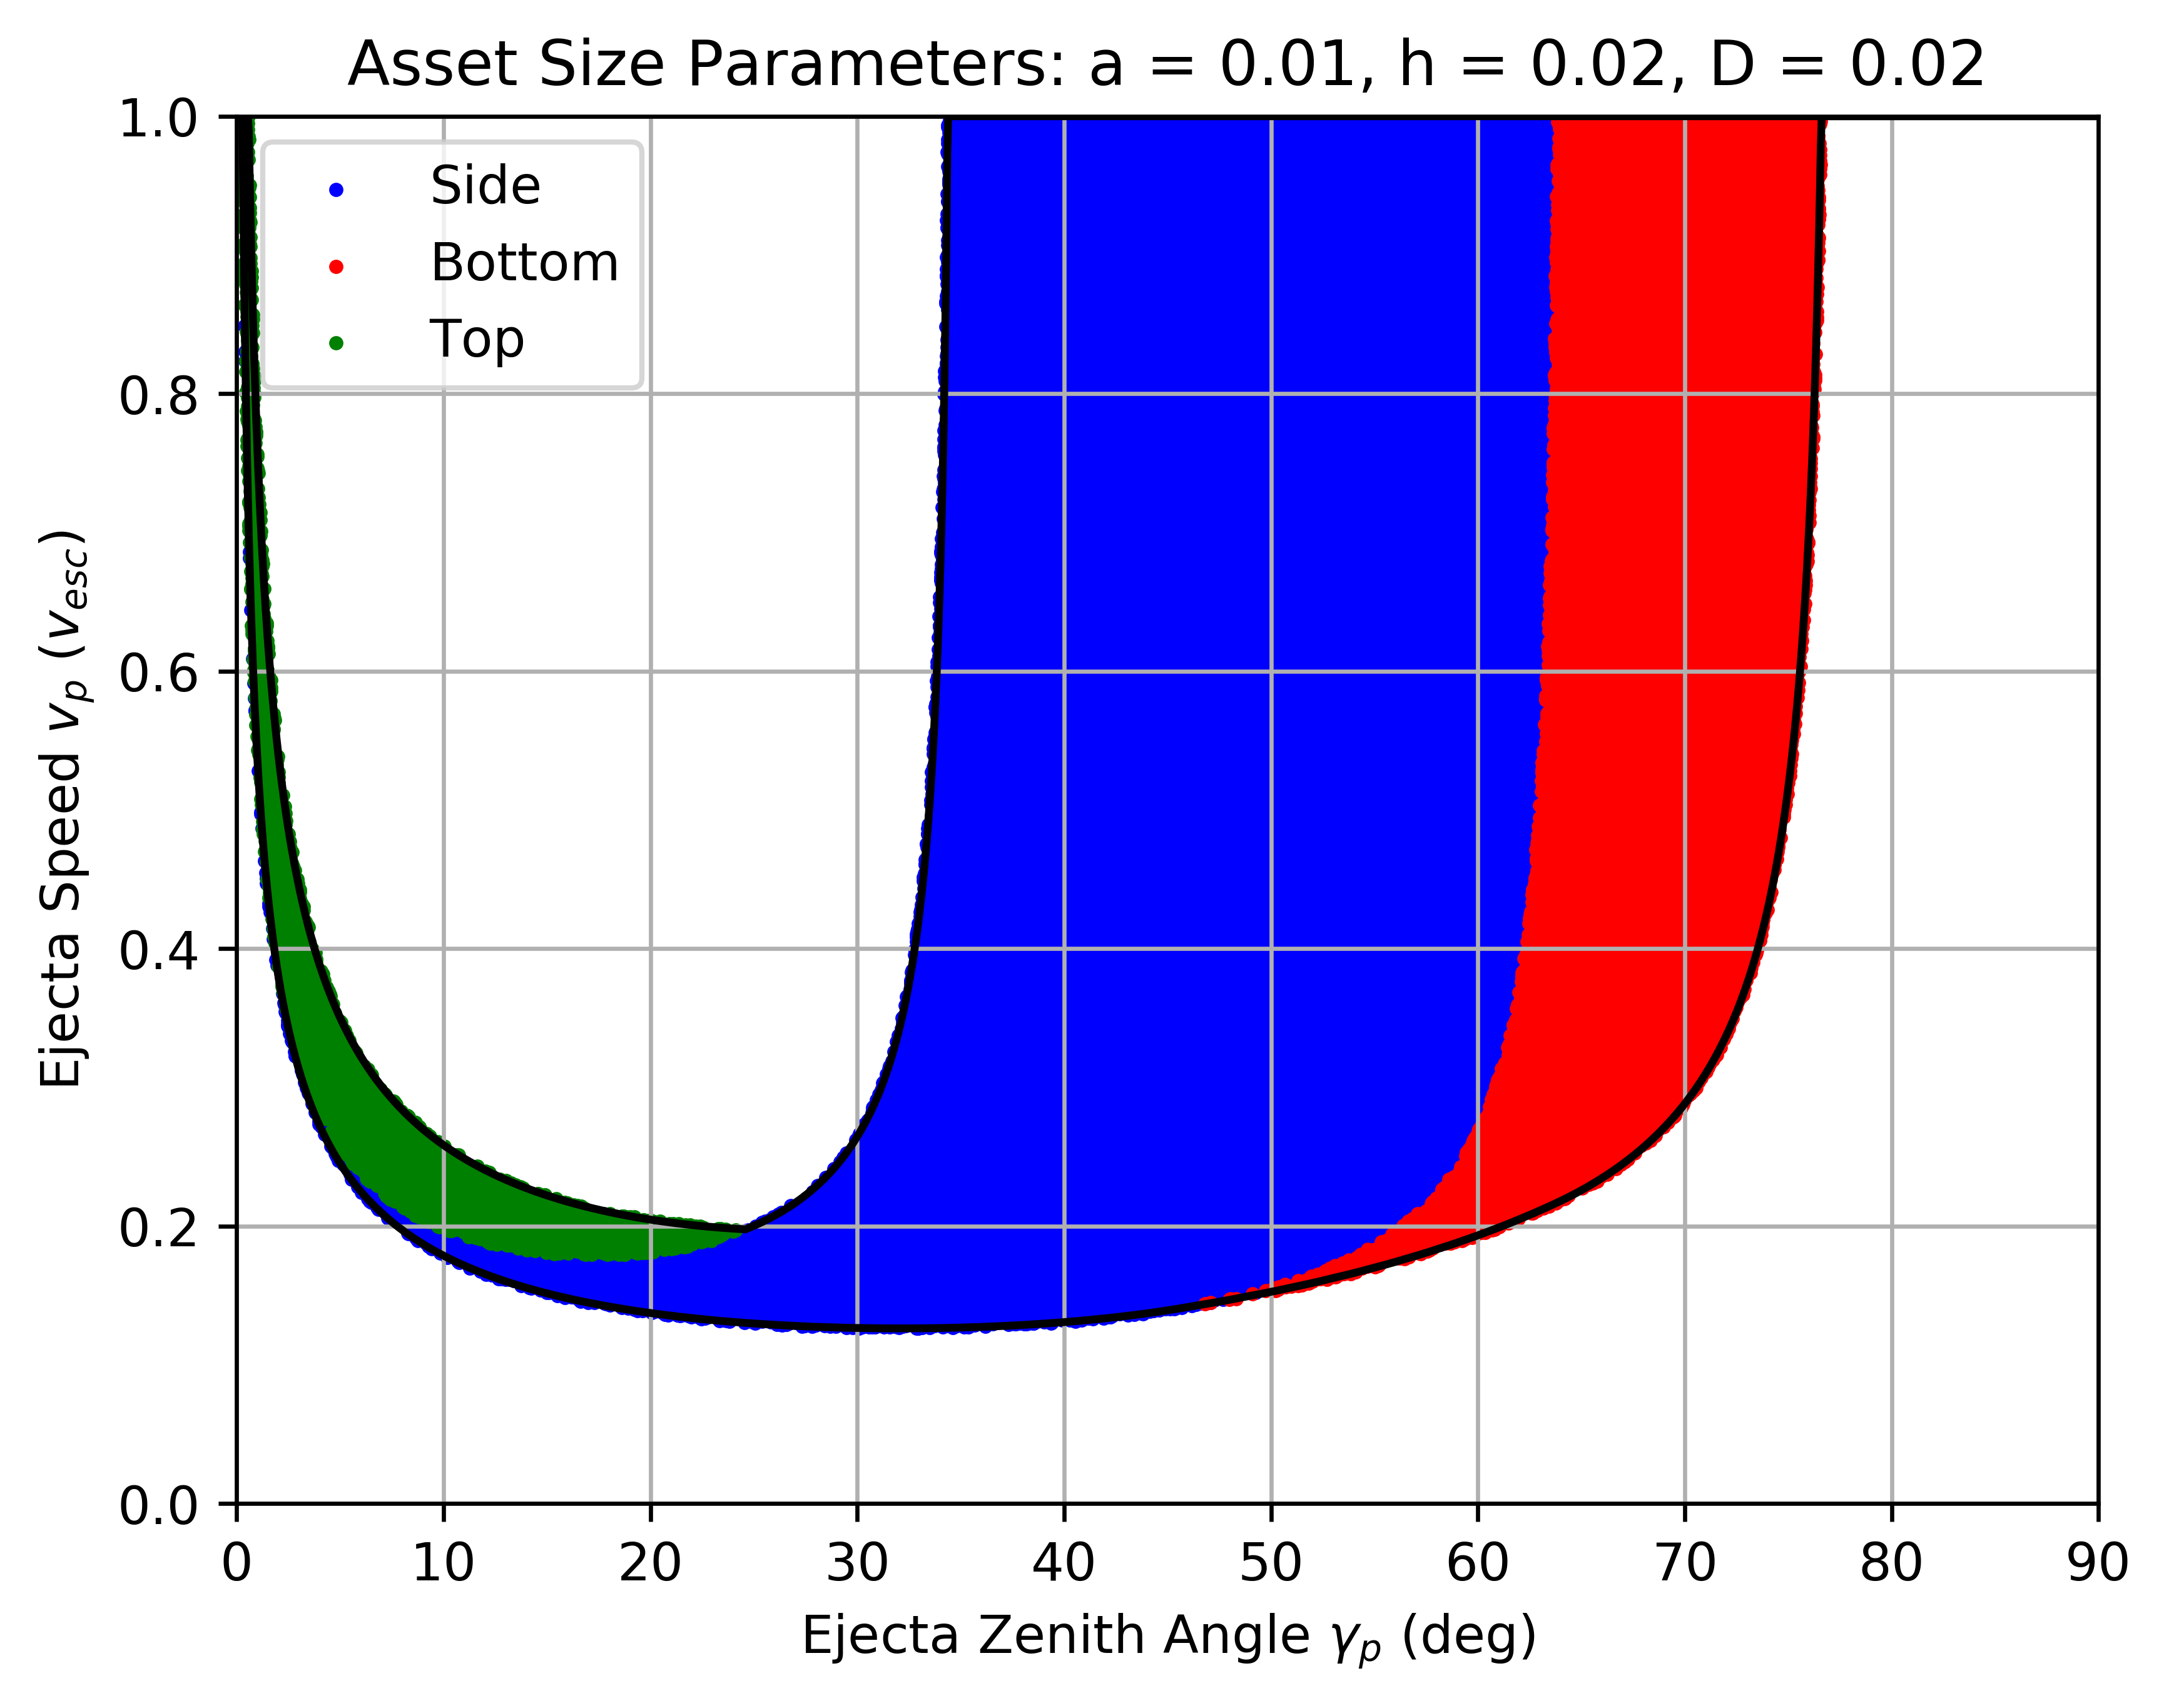
\includegraphics[width=.98\linewidth]{asset_speed_zenith_plot_1.010e+00_1.000e-02_2.000e-02_2.000e-02.png}  
		%\caption{Put your sub-caption here}
		\label{fig:sub-asset_speed_zenith_h1_5}
	\end{subfigure}
	\begin{subfigure}[t]{.32\textwidth}
		\centering
		% include fourth image
		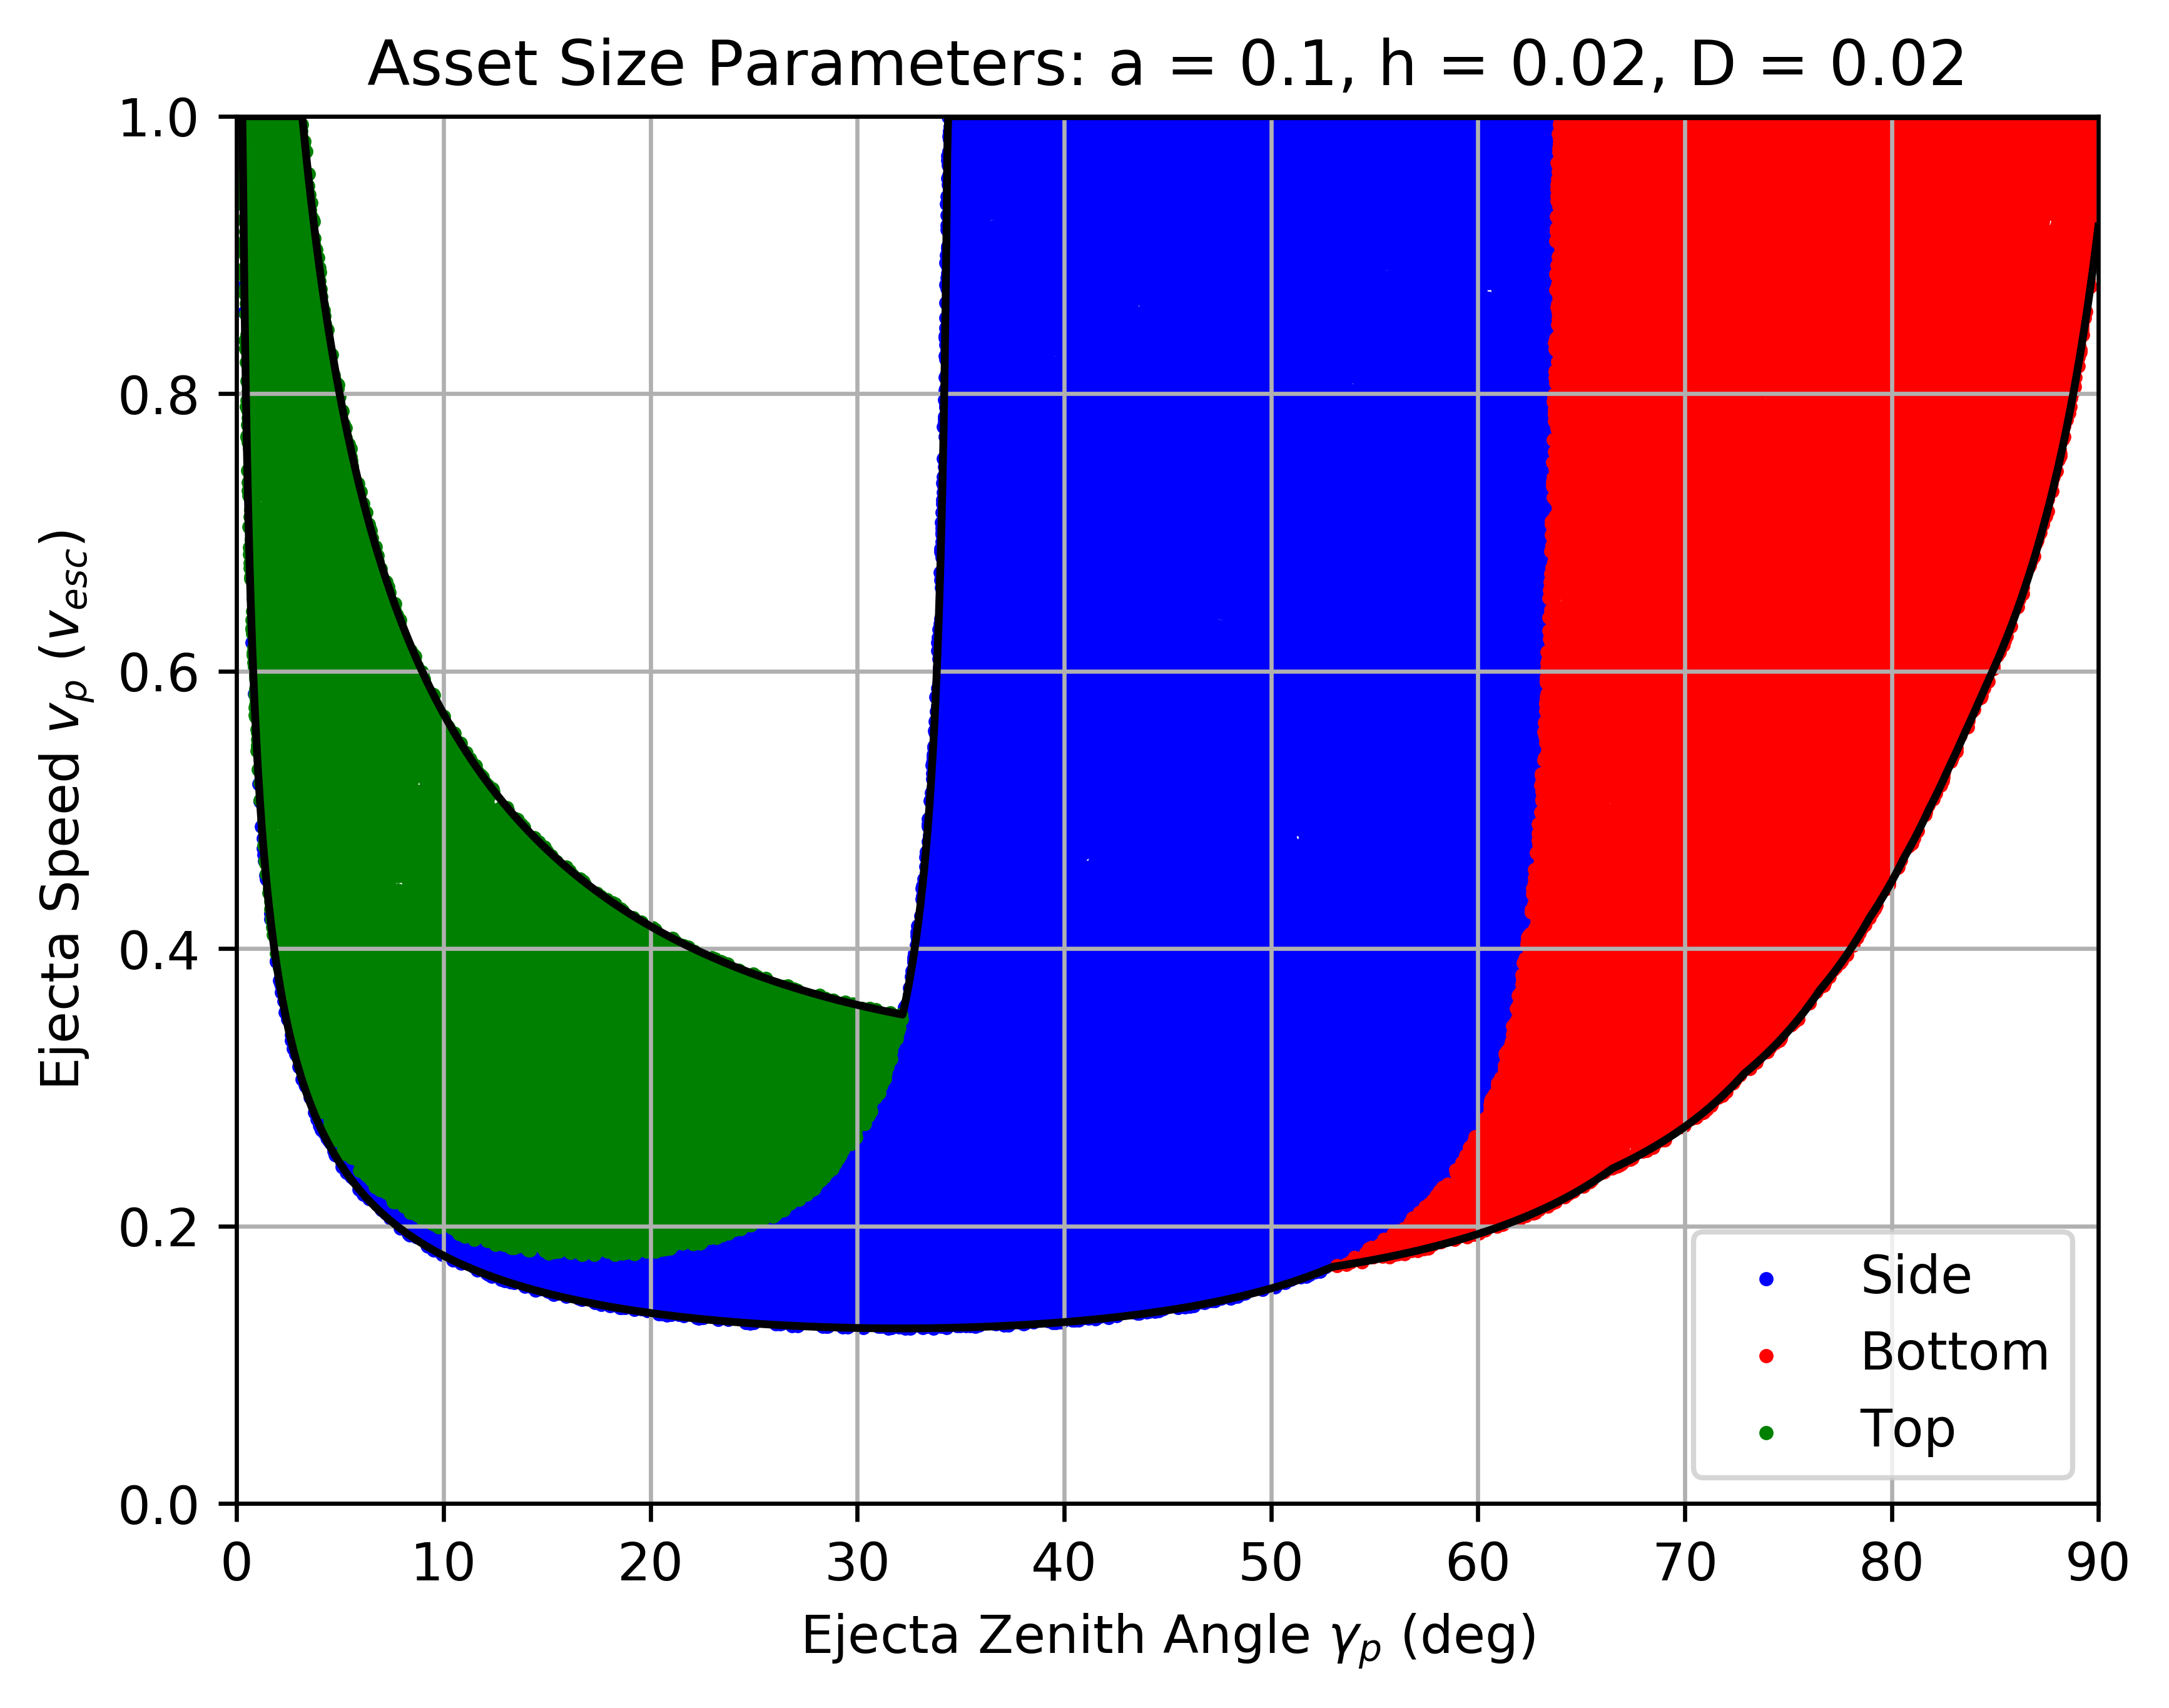
\includegraphics[width=.98\linewidth]{asset_speed_zenith_plot_1.010e+00_1.000e-01_2.000e-02_2.000e-02.png}  
		%\caption{Put your sub-caption here}
		\label{fig:sub-asset_speed_zenith_h1_6}
	\end{subfigure}
	
	
	\begin{subfigure}[t]{.32\textwidth}
		\centering
		% include third image
		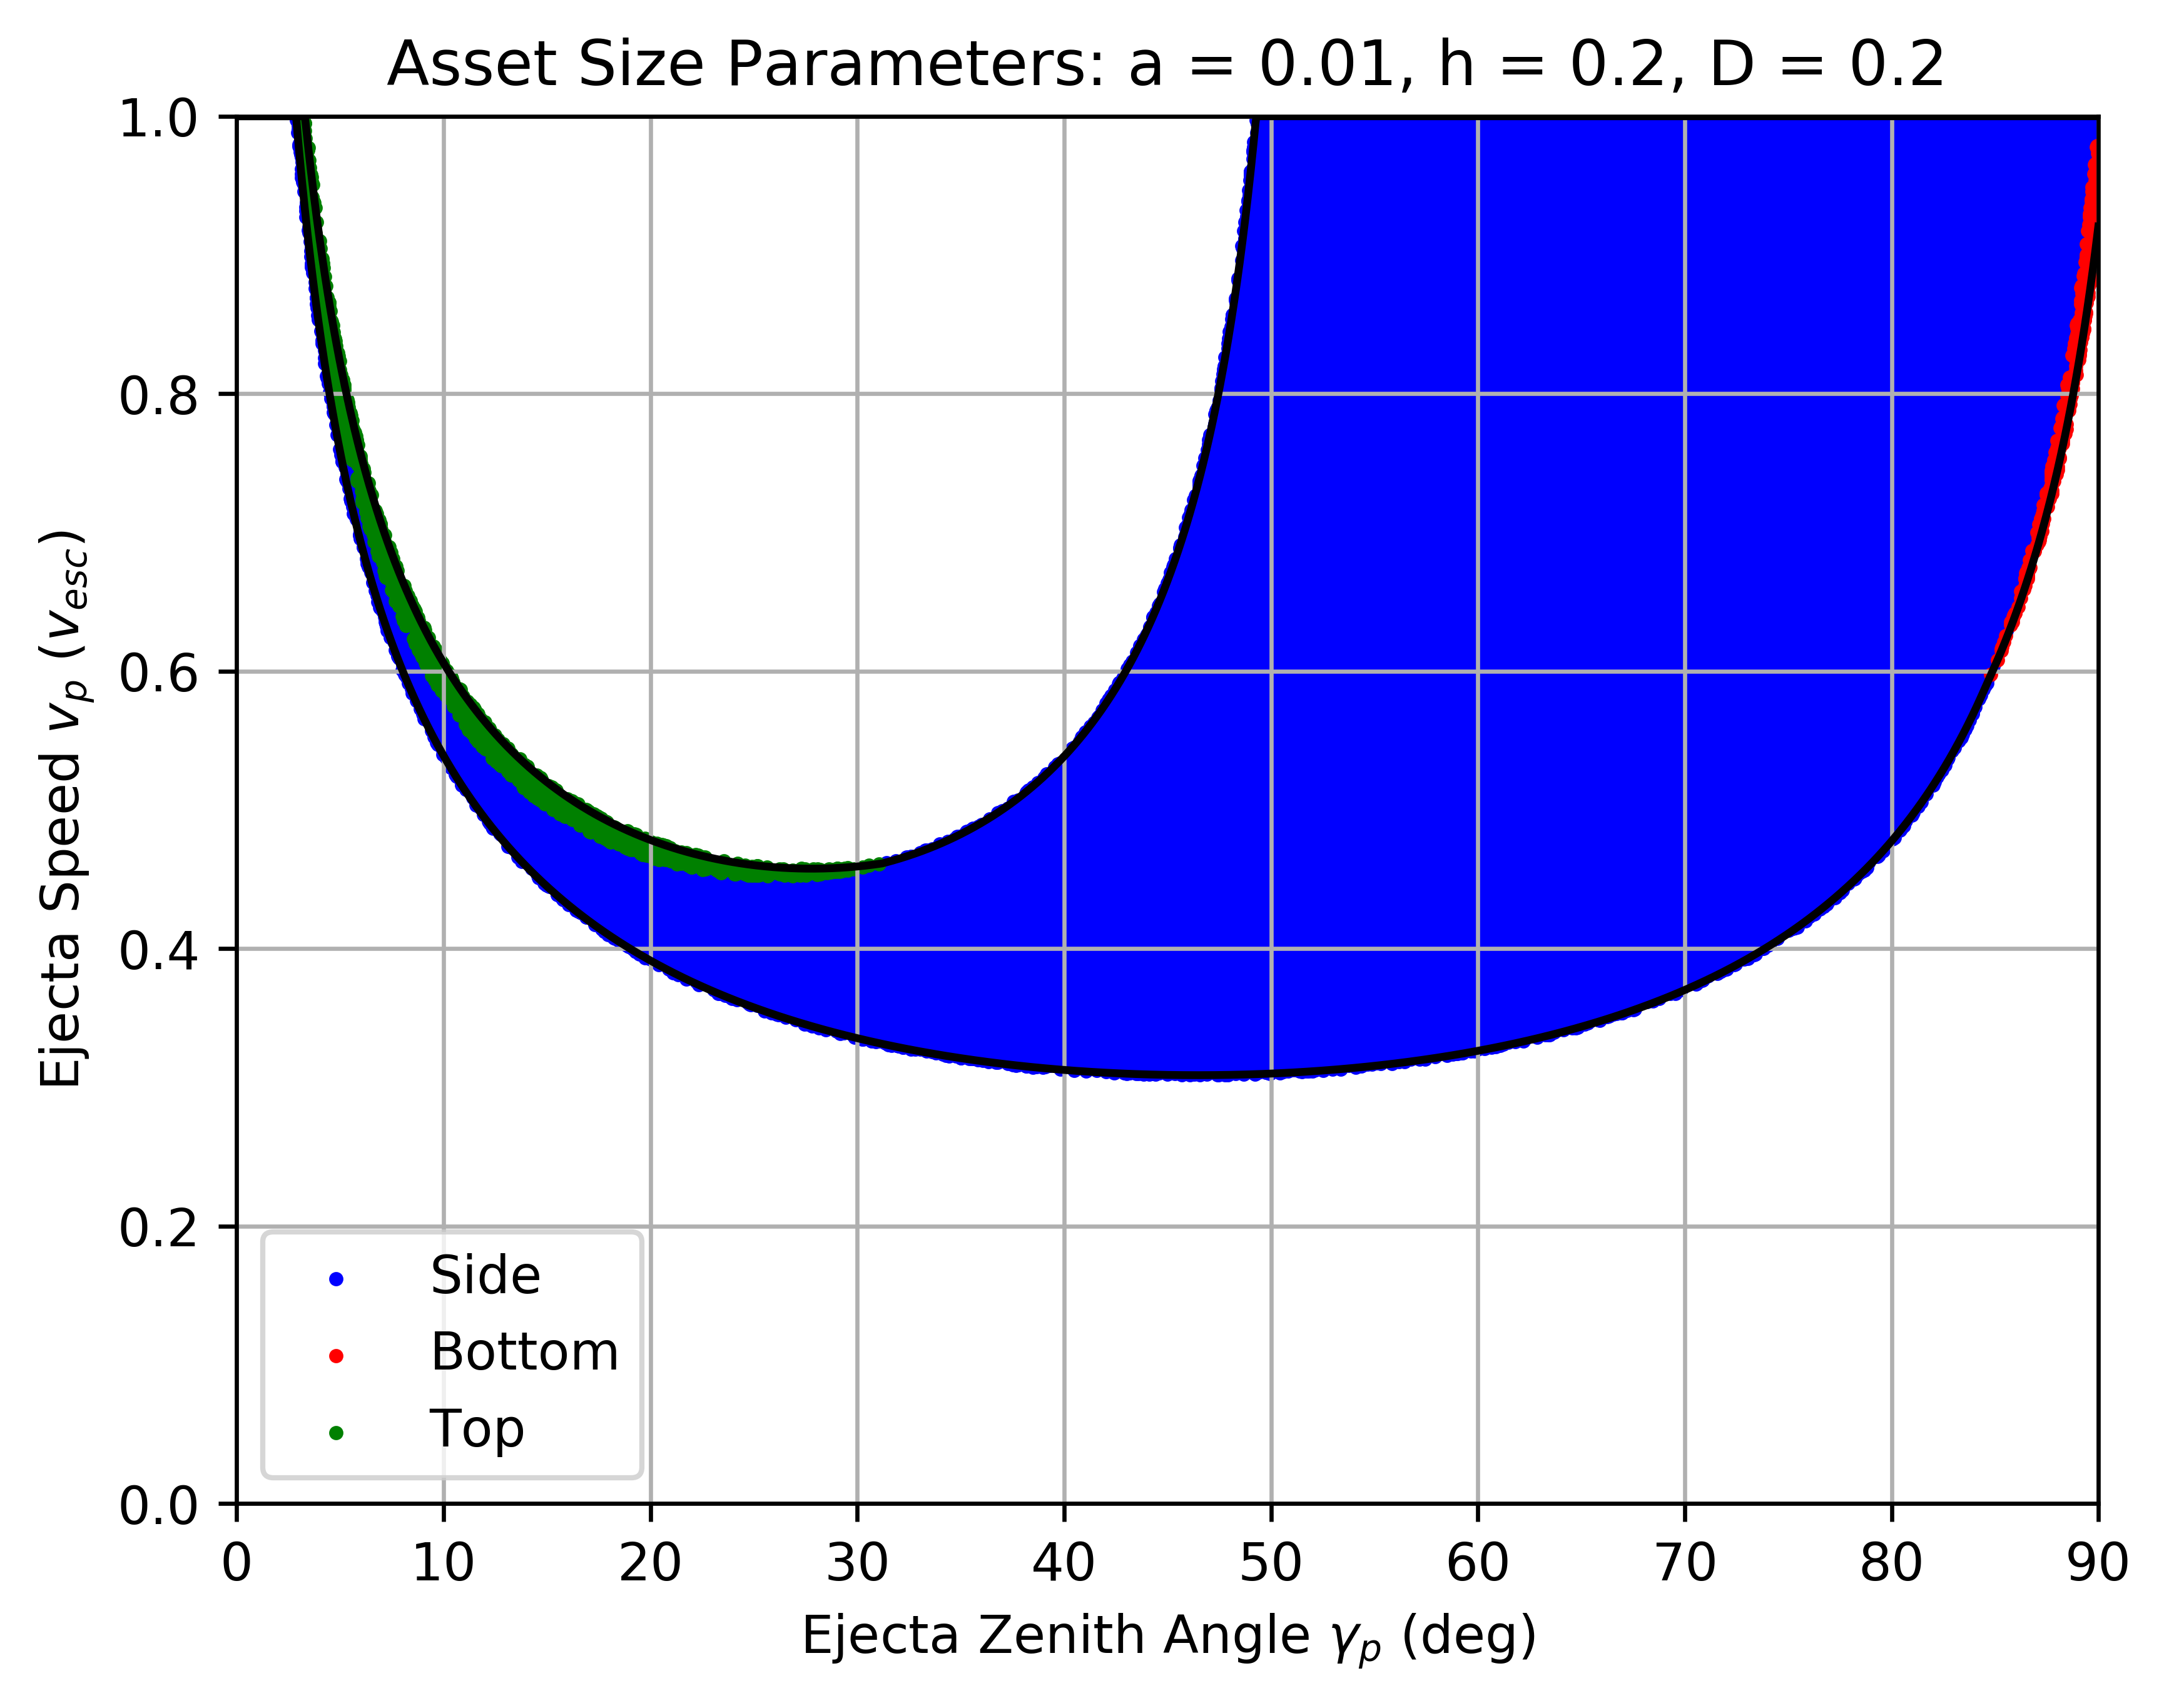
\includegraphics[width=.98\linewidth]{asset_speed_zenith_plot_1.010e+00_1.000e-02_2.000e-01_2.000e-01.png}  
		%\caption{Put your sub-caption here}
		\label{fig:sub-asset_speed_zenith_h1_7}
	\end{subfigure}
	\begin{subfigure}[t]{.32\textwidth}
		\centering
		% include fourth image
		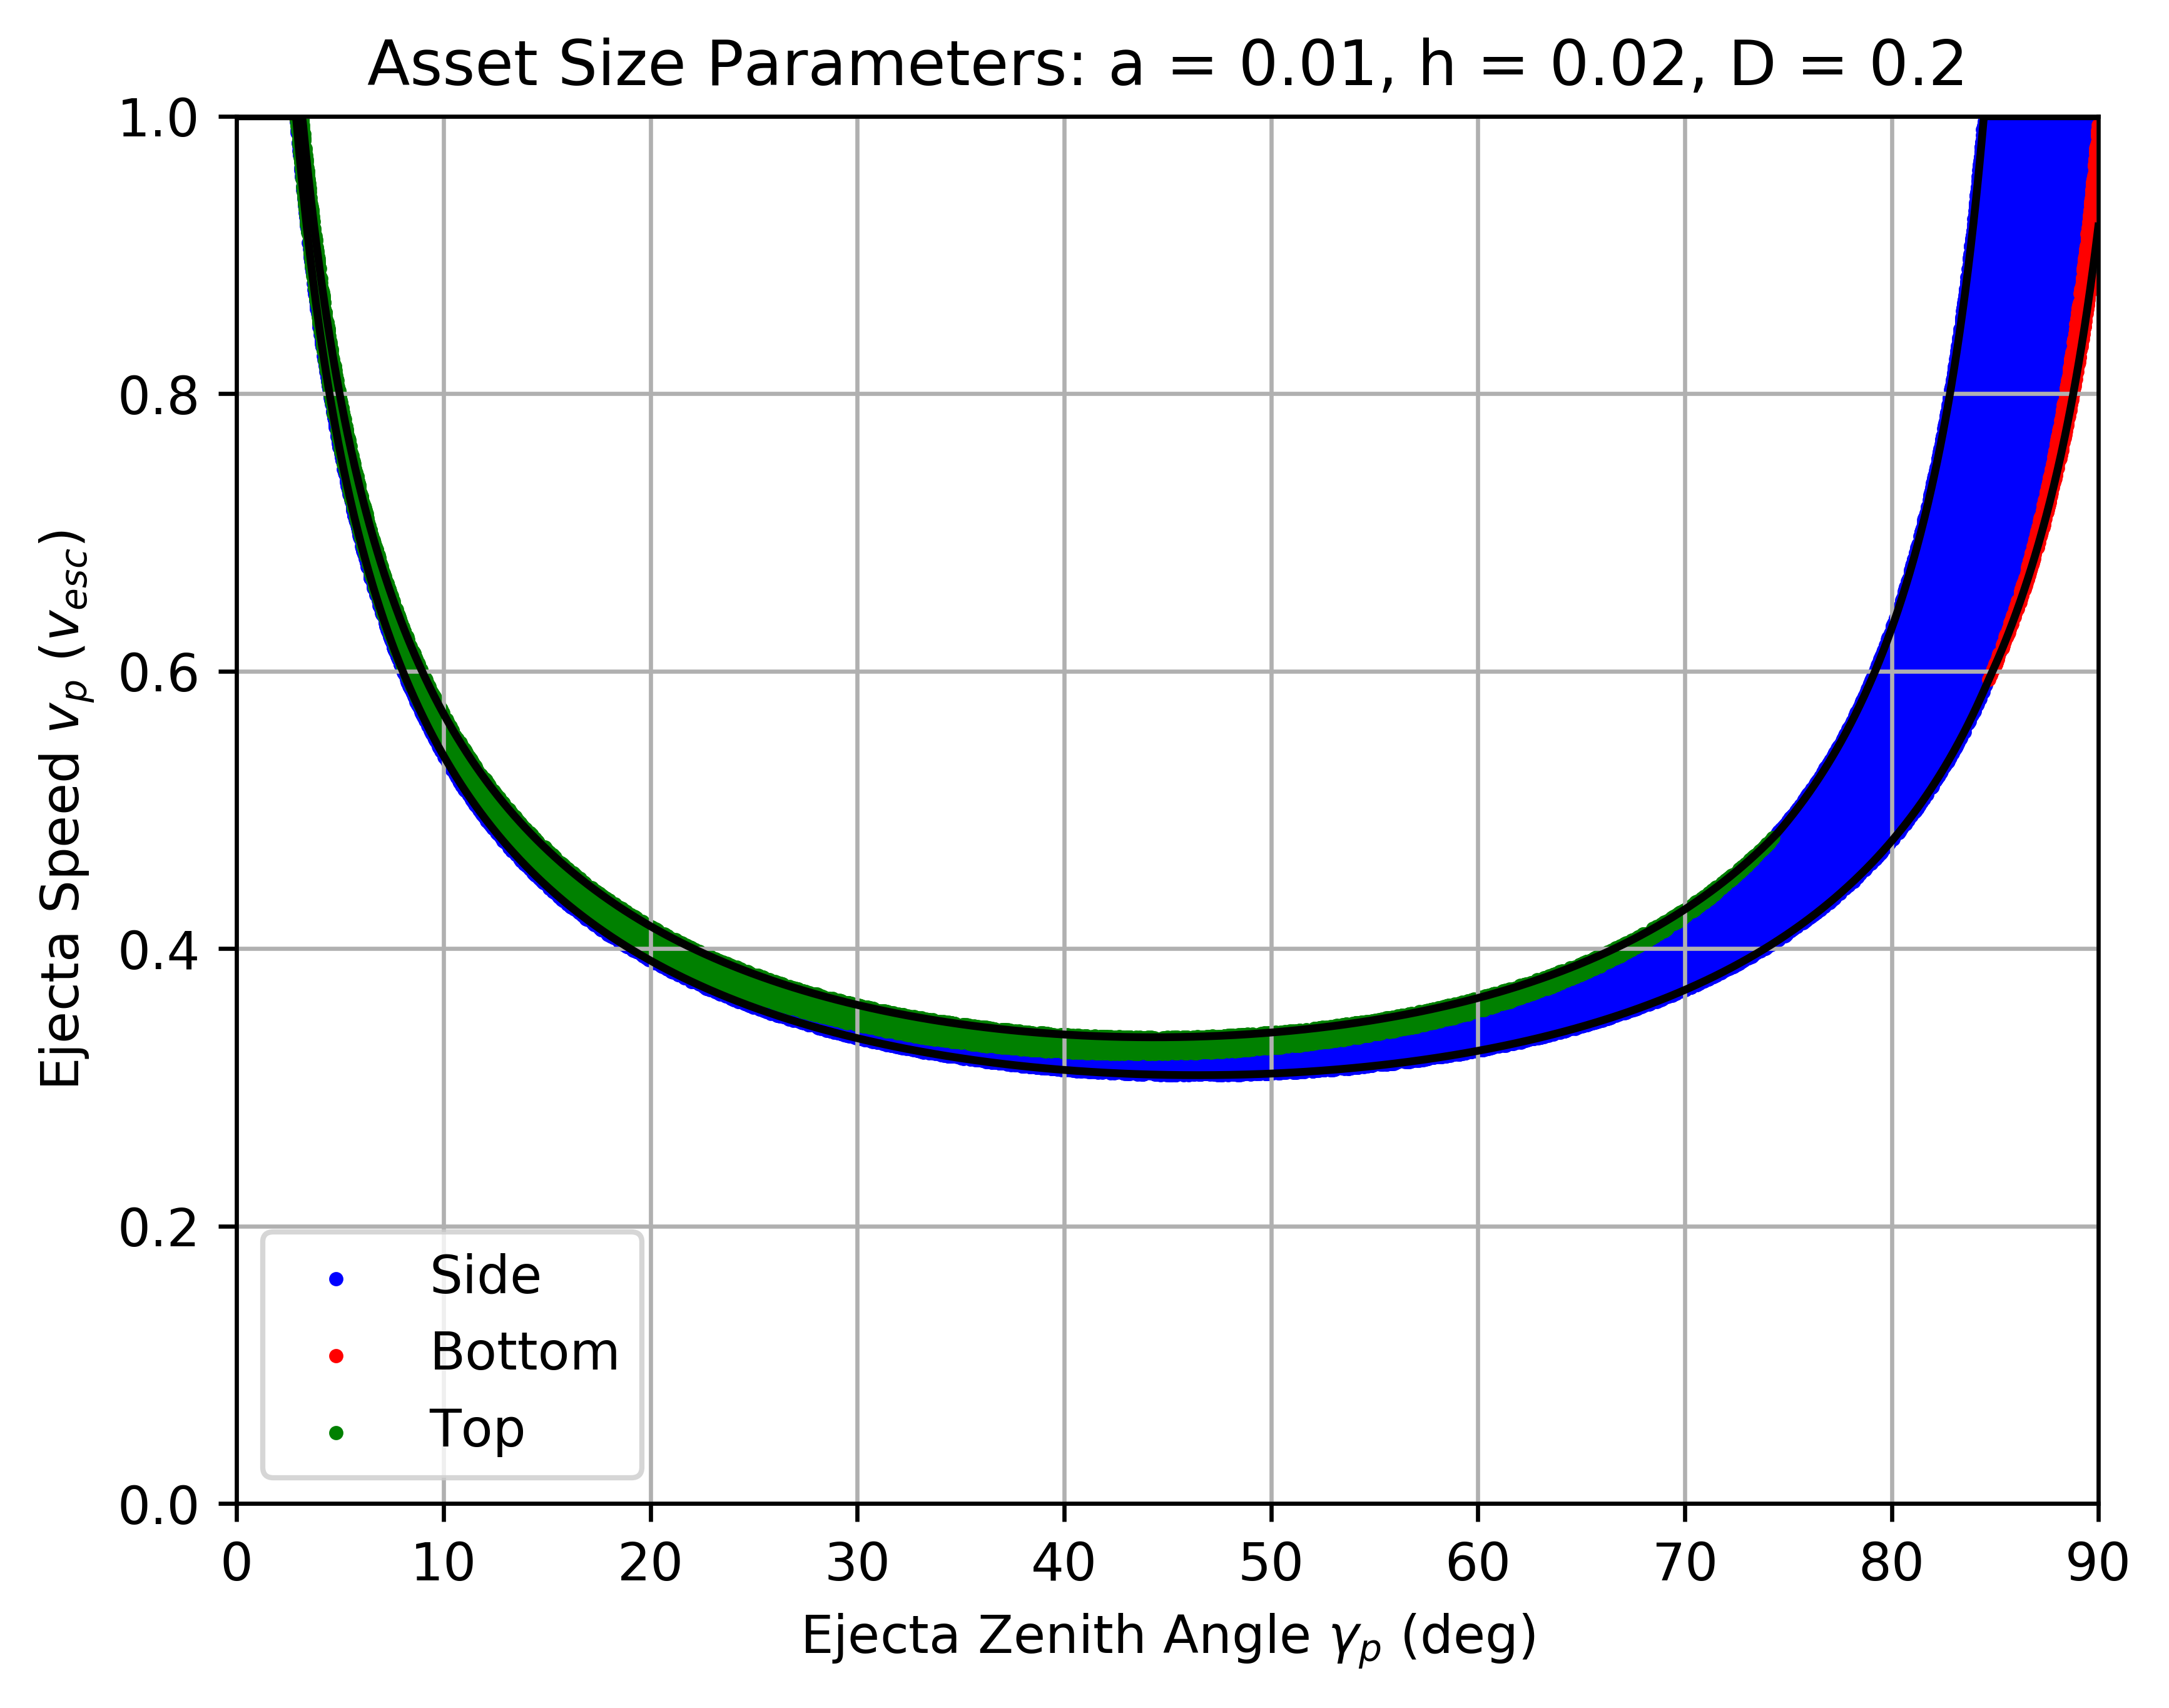
\includegraphics[width=.98\linewidth]{asset_speed_zenith_plot_1.010e+00_1.000e-02_2.000e-02_2.000e-01.png}  
		%\caption{Put your sub-caption here}
		\label{fig:sub-asset_speed_zenith_h1_8}
	\end{subfigure}
	\begin{subfigure}[t]{.32\textwidth}
		\centering
		% include fourth image
		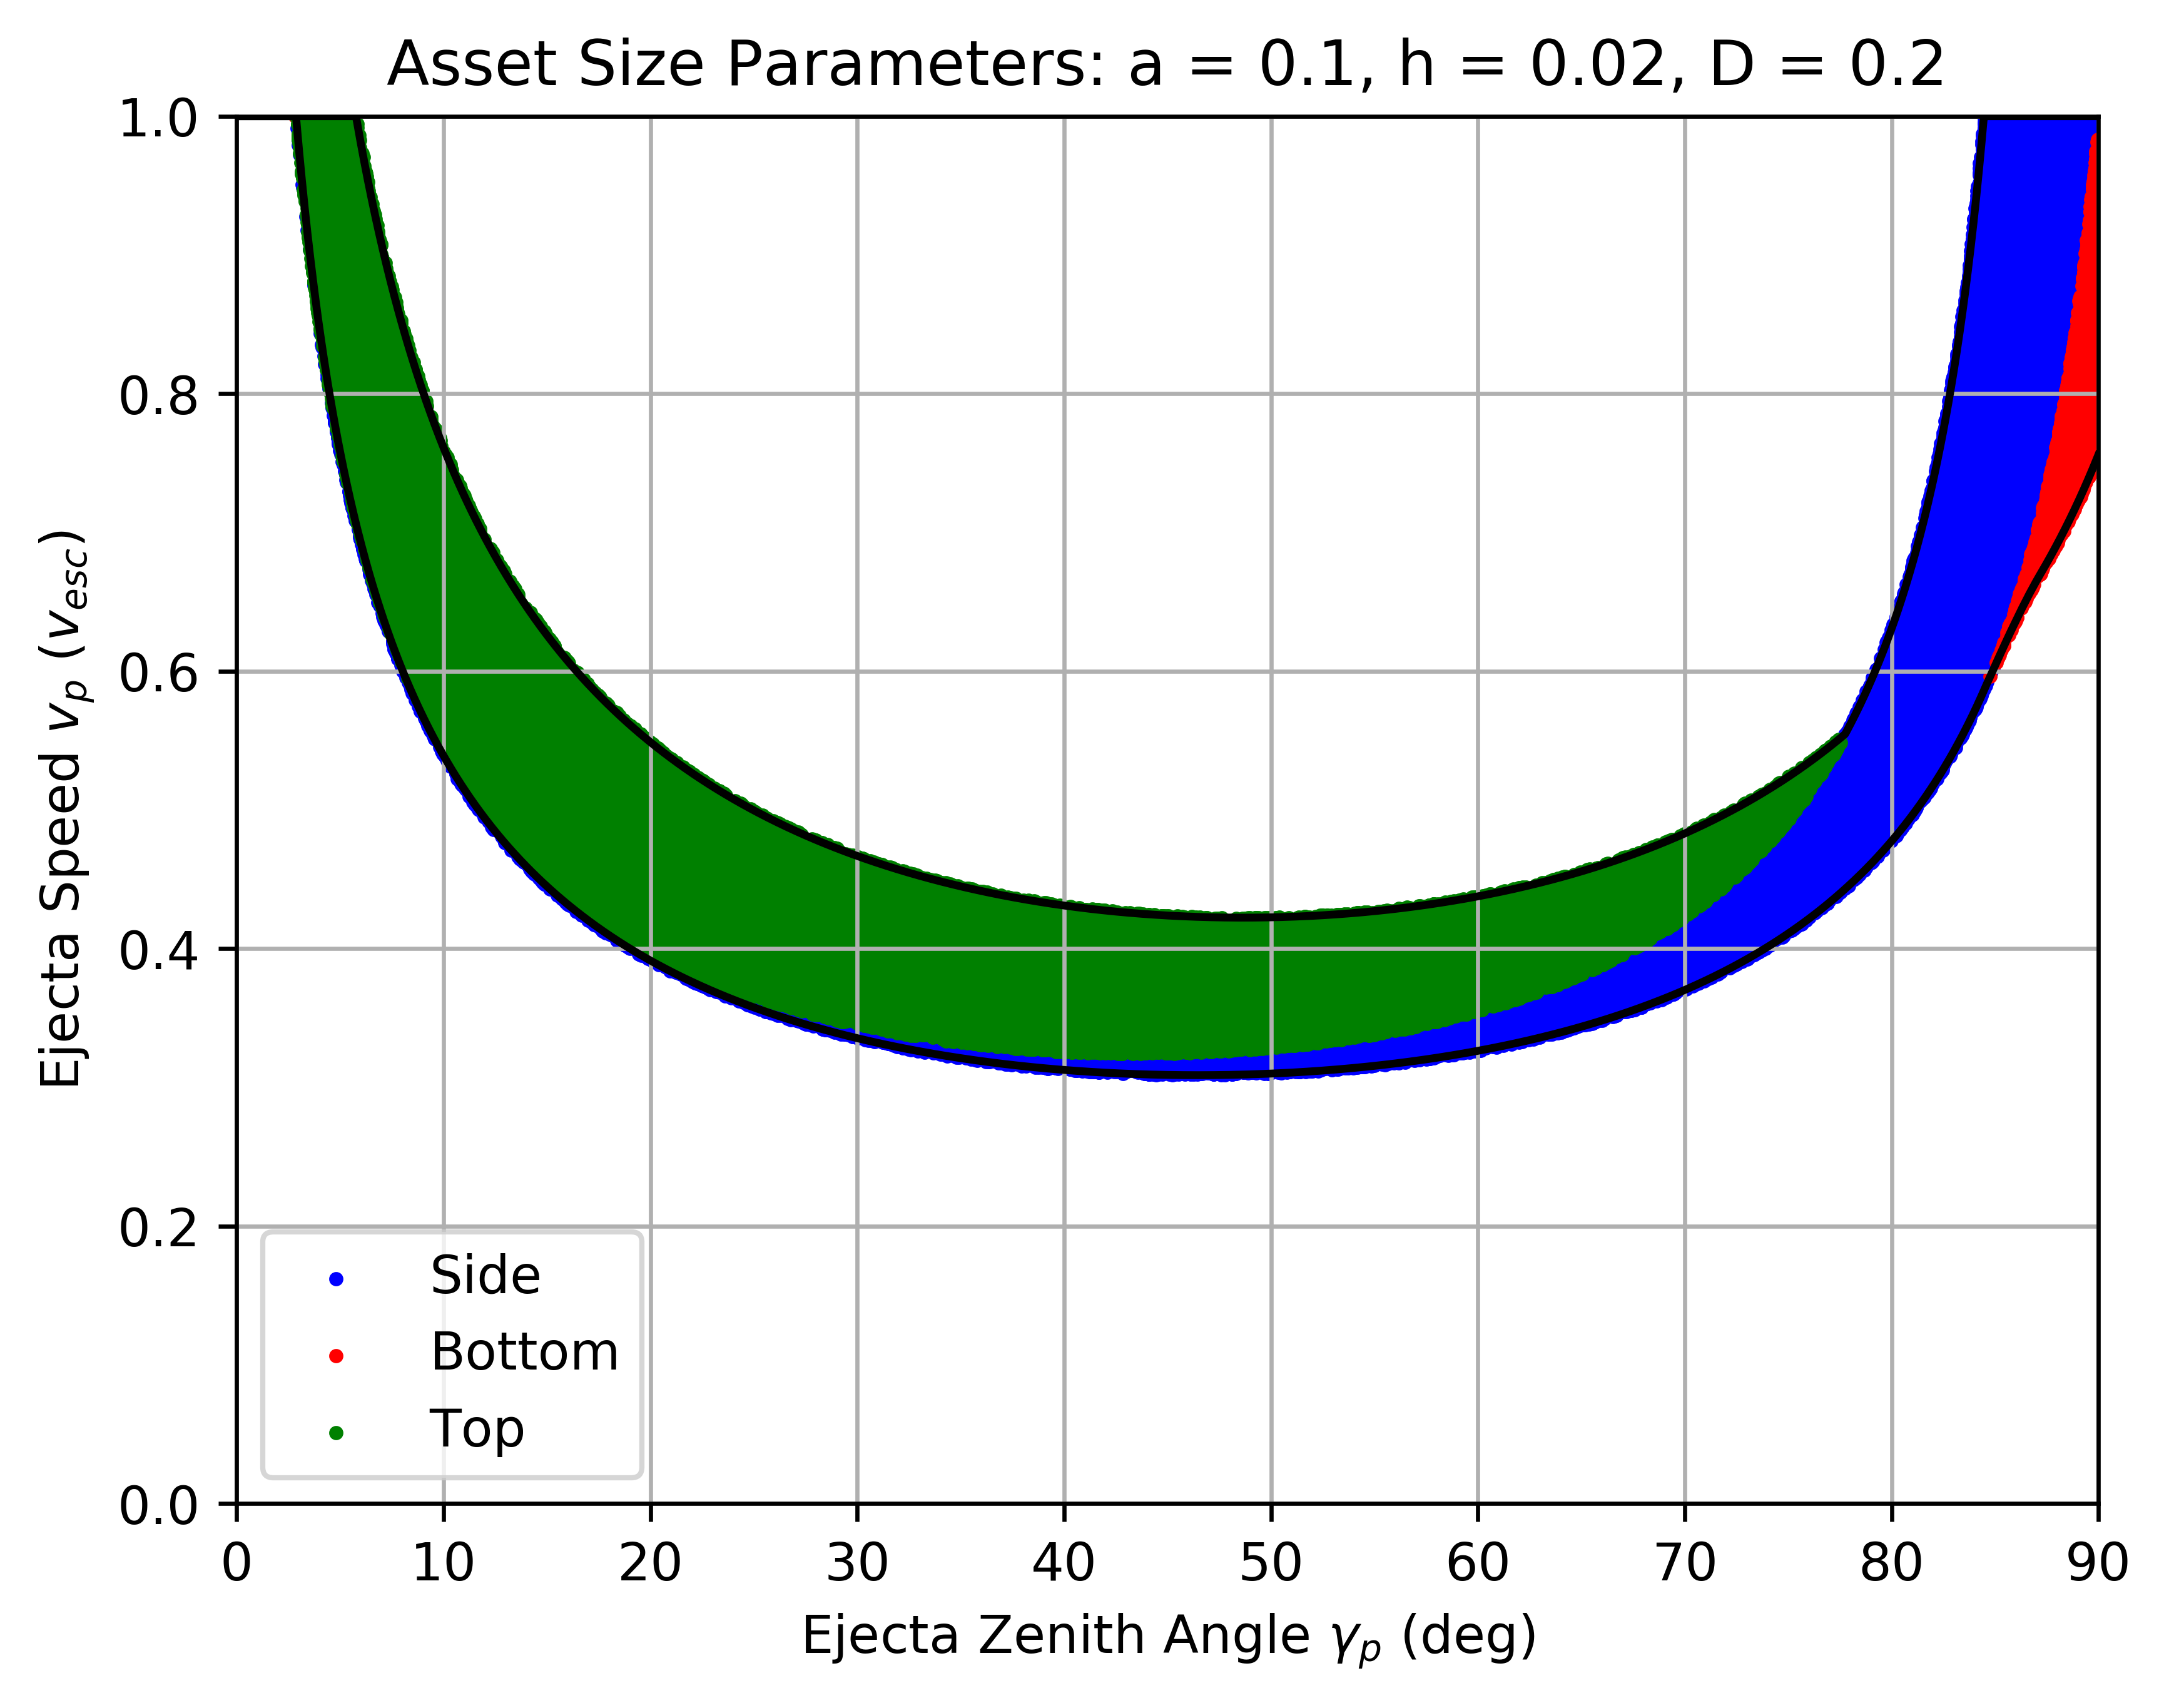
\includegraphics[width=.98\linewidth]{asset_speed_zenith_plot_1.010e+00_1.000e-01_2.000e-02_2.000e-01.png}  
		%\caption{Put your sub-caption here}
		\label{fig:sub-asset_speed_zenith_h1_9}
	\end{subfigure}
	
	\begin{subfigure}[t]{.32\textwidth}
		\centering
		% include third image
		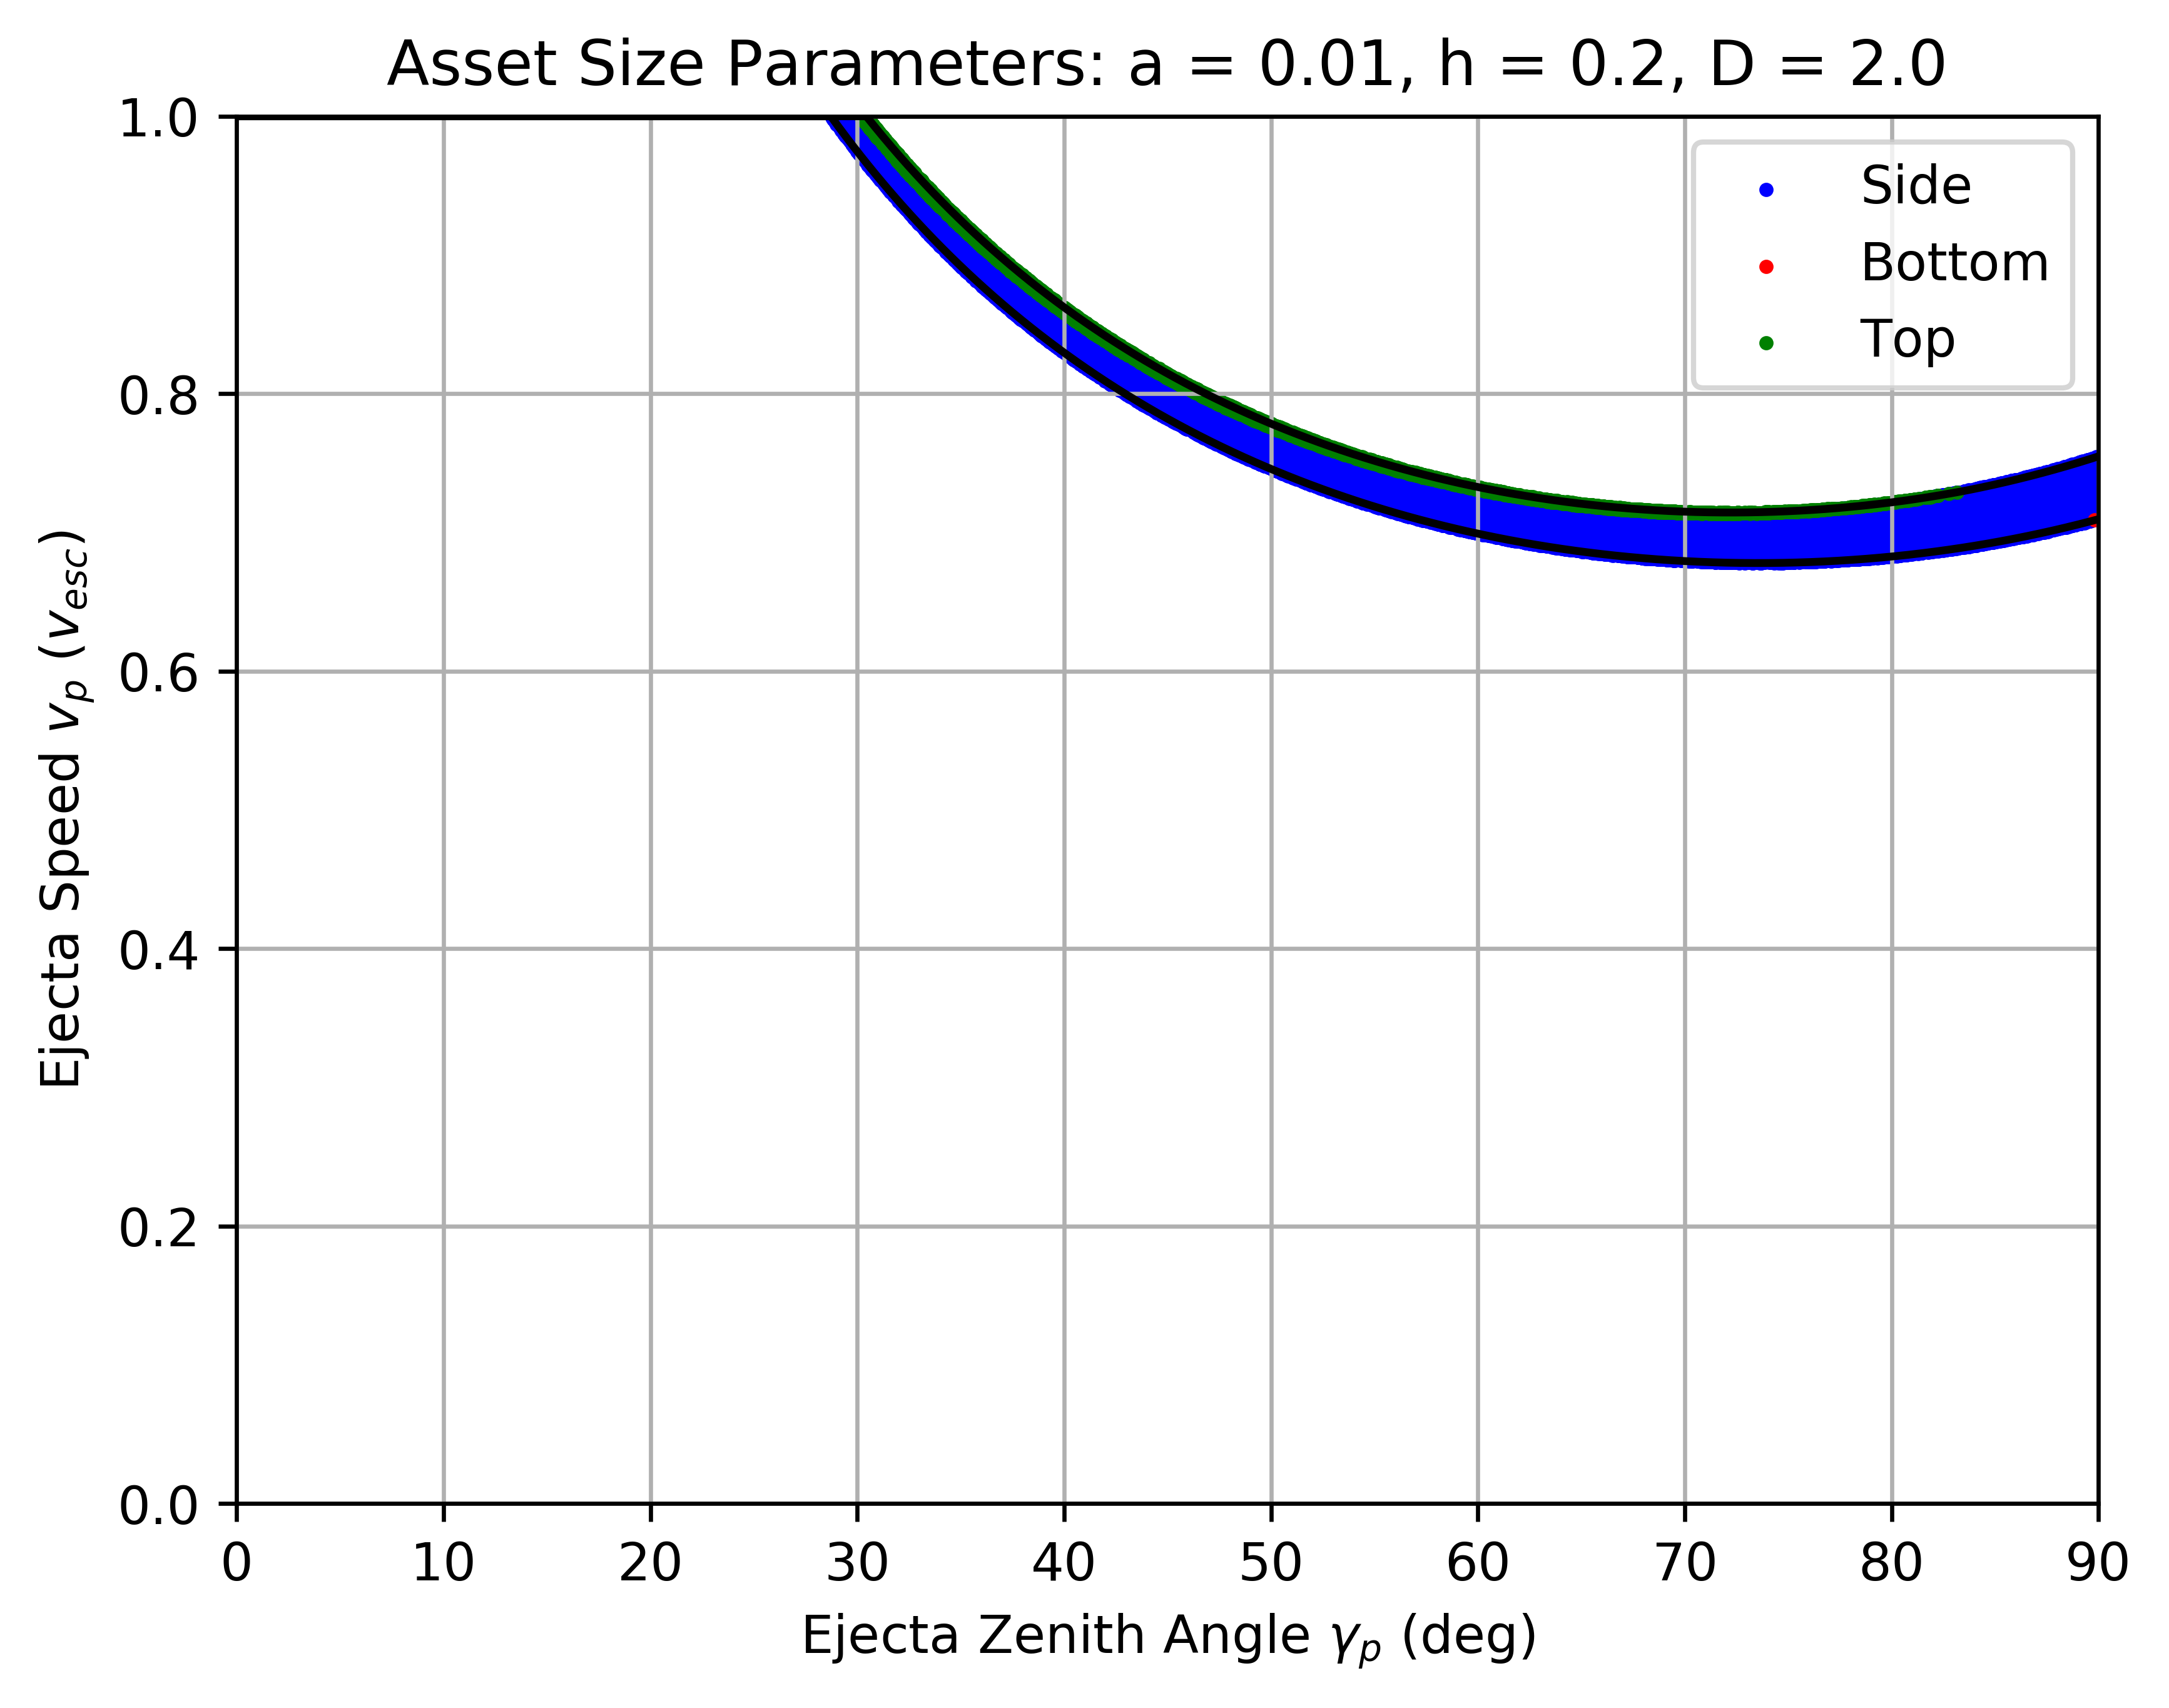
\includegraphics[width=.98\linewidth]{asset_speed_zenith_plot_1.010e+00_1.000e-02_2.000e-01_2.000e+00.png}  
		%\caption{Put your sub-caption here}
		\label{fig:sub-asset_speed_zenith_h1_10}
	\end{subfigure}
	\begin{subfigure}[t]{.32\textwidth}
		\centering
		% include fourth image
		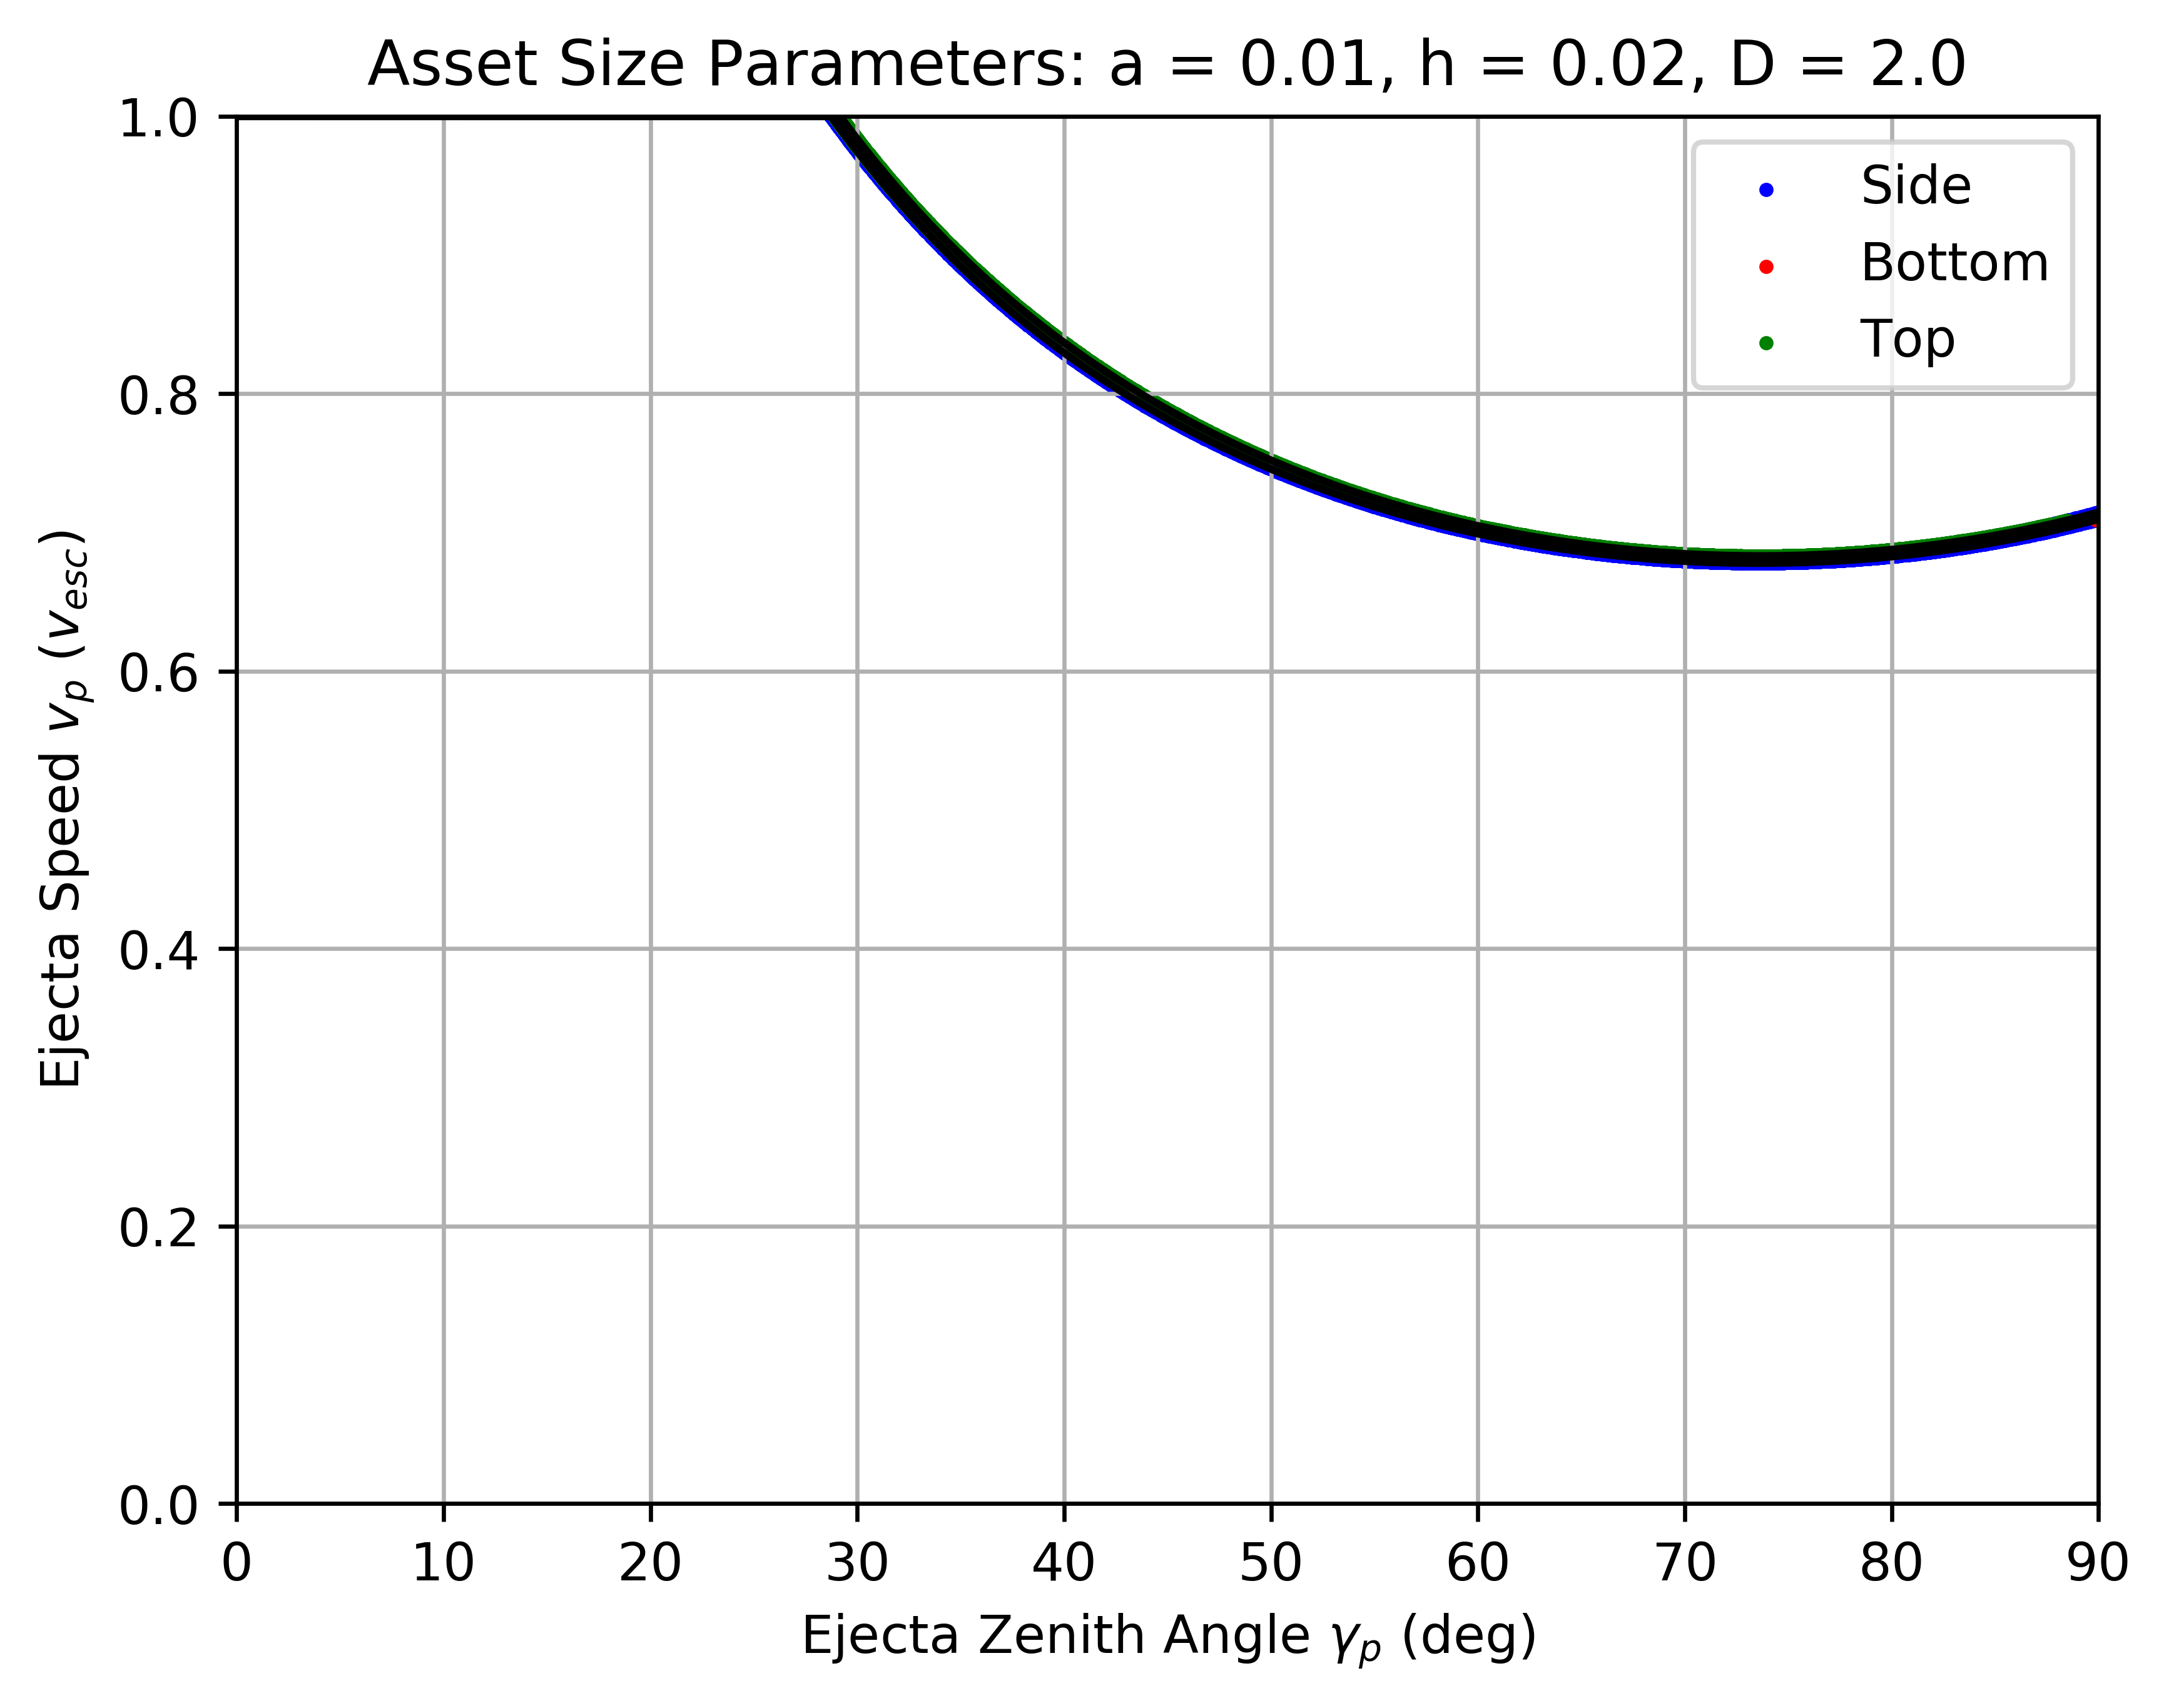
\includegraphics[width=.98\linewidth]{asset_speed_zenith_plot_1.010e+00_1.000e-02_2.000e-02_2.000e+00.png}  
		%\caption{Put your sub-caption here}
		\label{fig:sub-asset_speed_zenith_h1_11}
	\end{subfigure}
	\begin{subfigure}[t]{.32\textwidth}
		\centering
		% include fourth image
		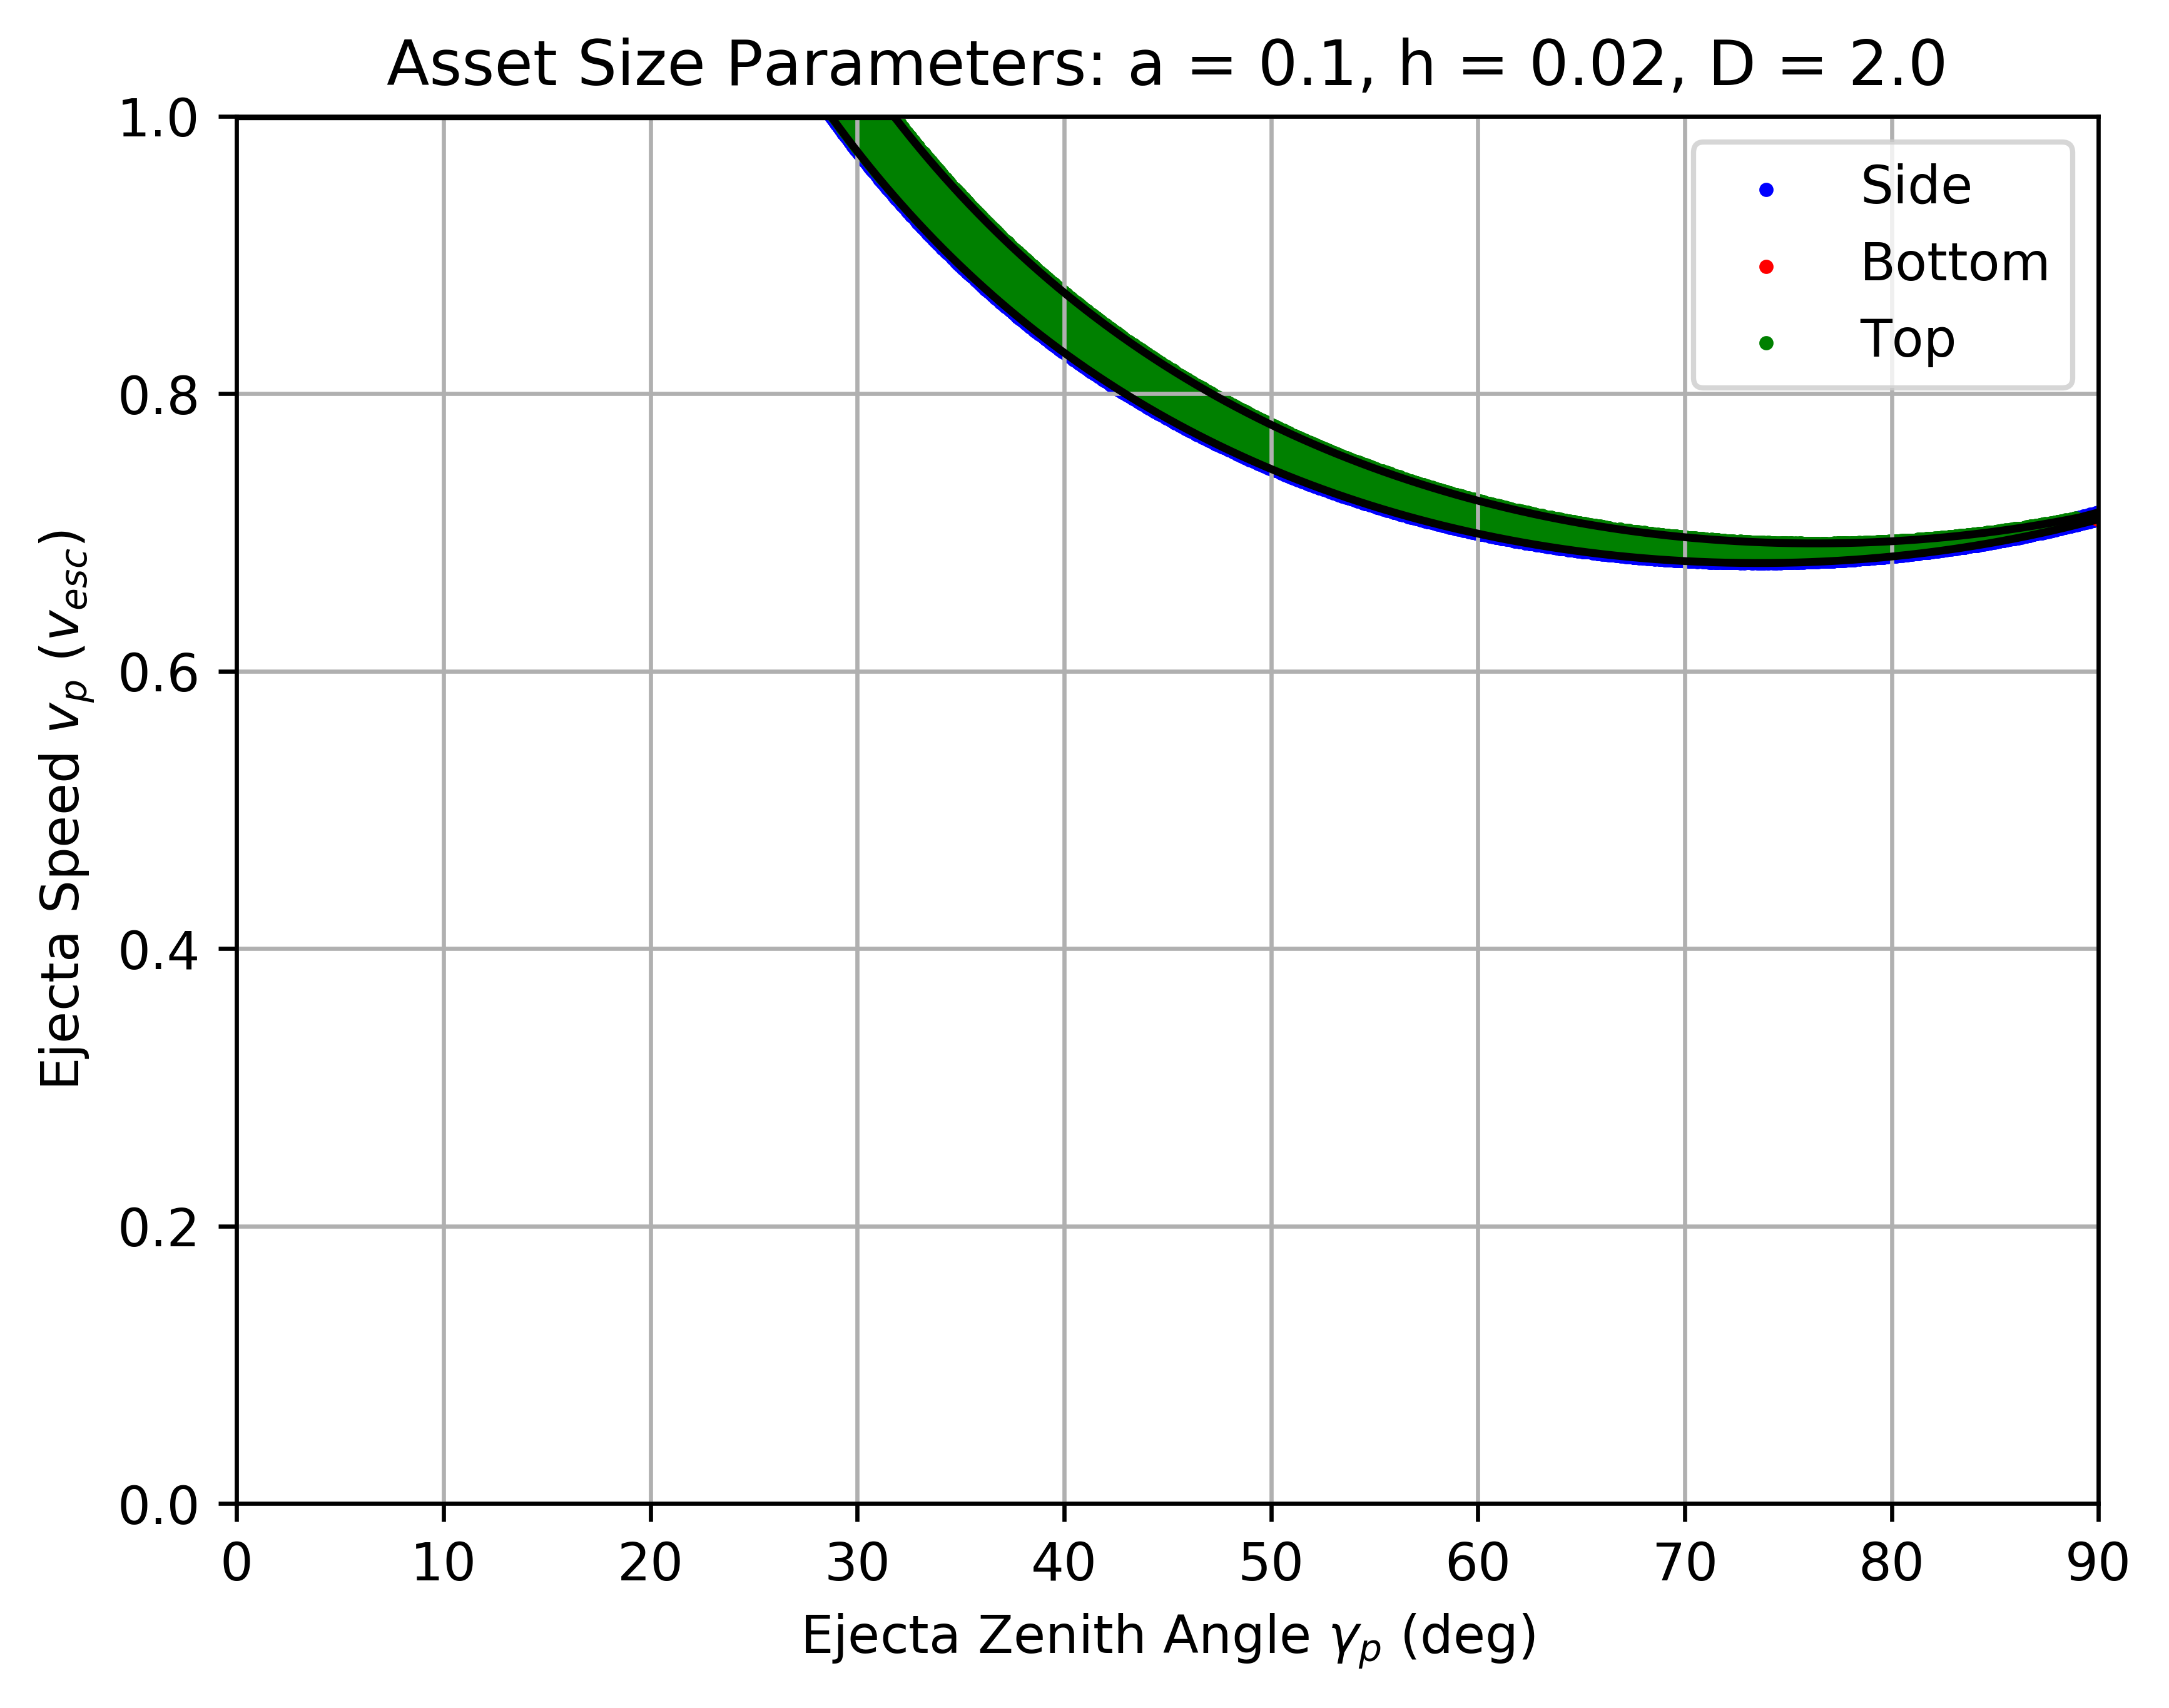
\includegraphics[width=.98\linewidth]{asset_speed_zenith_plot_1.010e+00_1.000e-01_2.000e-02_2.000e+00.png}  
		%\caption{Put your sub-caption here}
		\label{fig:sub-asset_speed_zenith_h1_12}
	\end{subfigure}
	
	\caption{A matrix of plots showing the ejecta hitting a cylindrical asset (in a plane intersecting the cylinder's symmetry axis) with a height above the surface of $0.01 r_m$ for various asset sizes and crater-to-asset distances. Each plot gives three colors for the ejecta hitting the side (blue), bottom (red), and the top (green) as a function of initial ejecta speed $v_p$ vs.\ initial ejecta zenith angle $\gamma_p$.}
	\label{fig:asset_speed_zenith_comparison_h1}
\end{figure}








\begin{figure}
	\begin{subfigure}[t]{.32\textwidth}
		\centering
		% include first image
		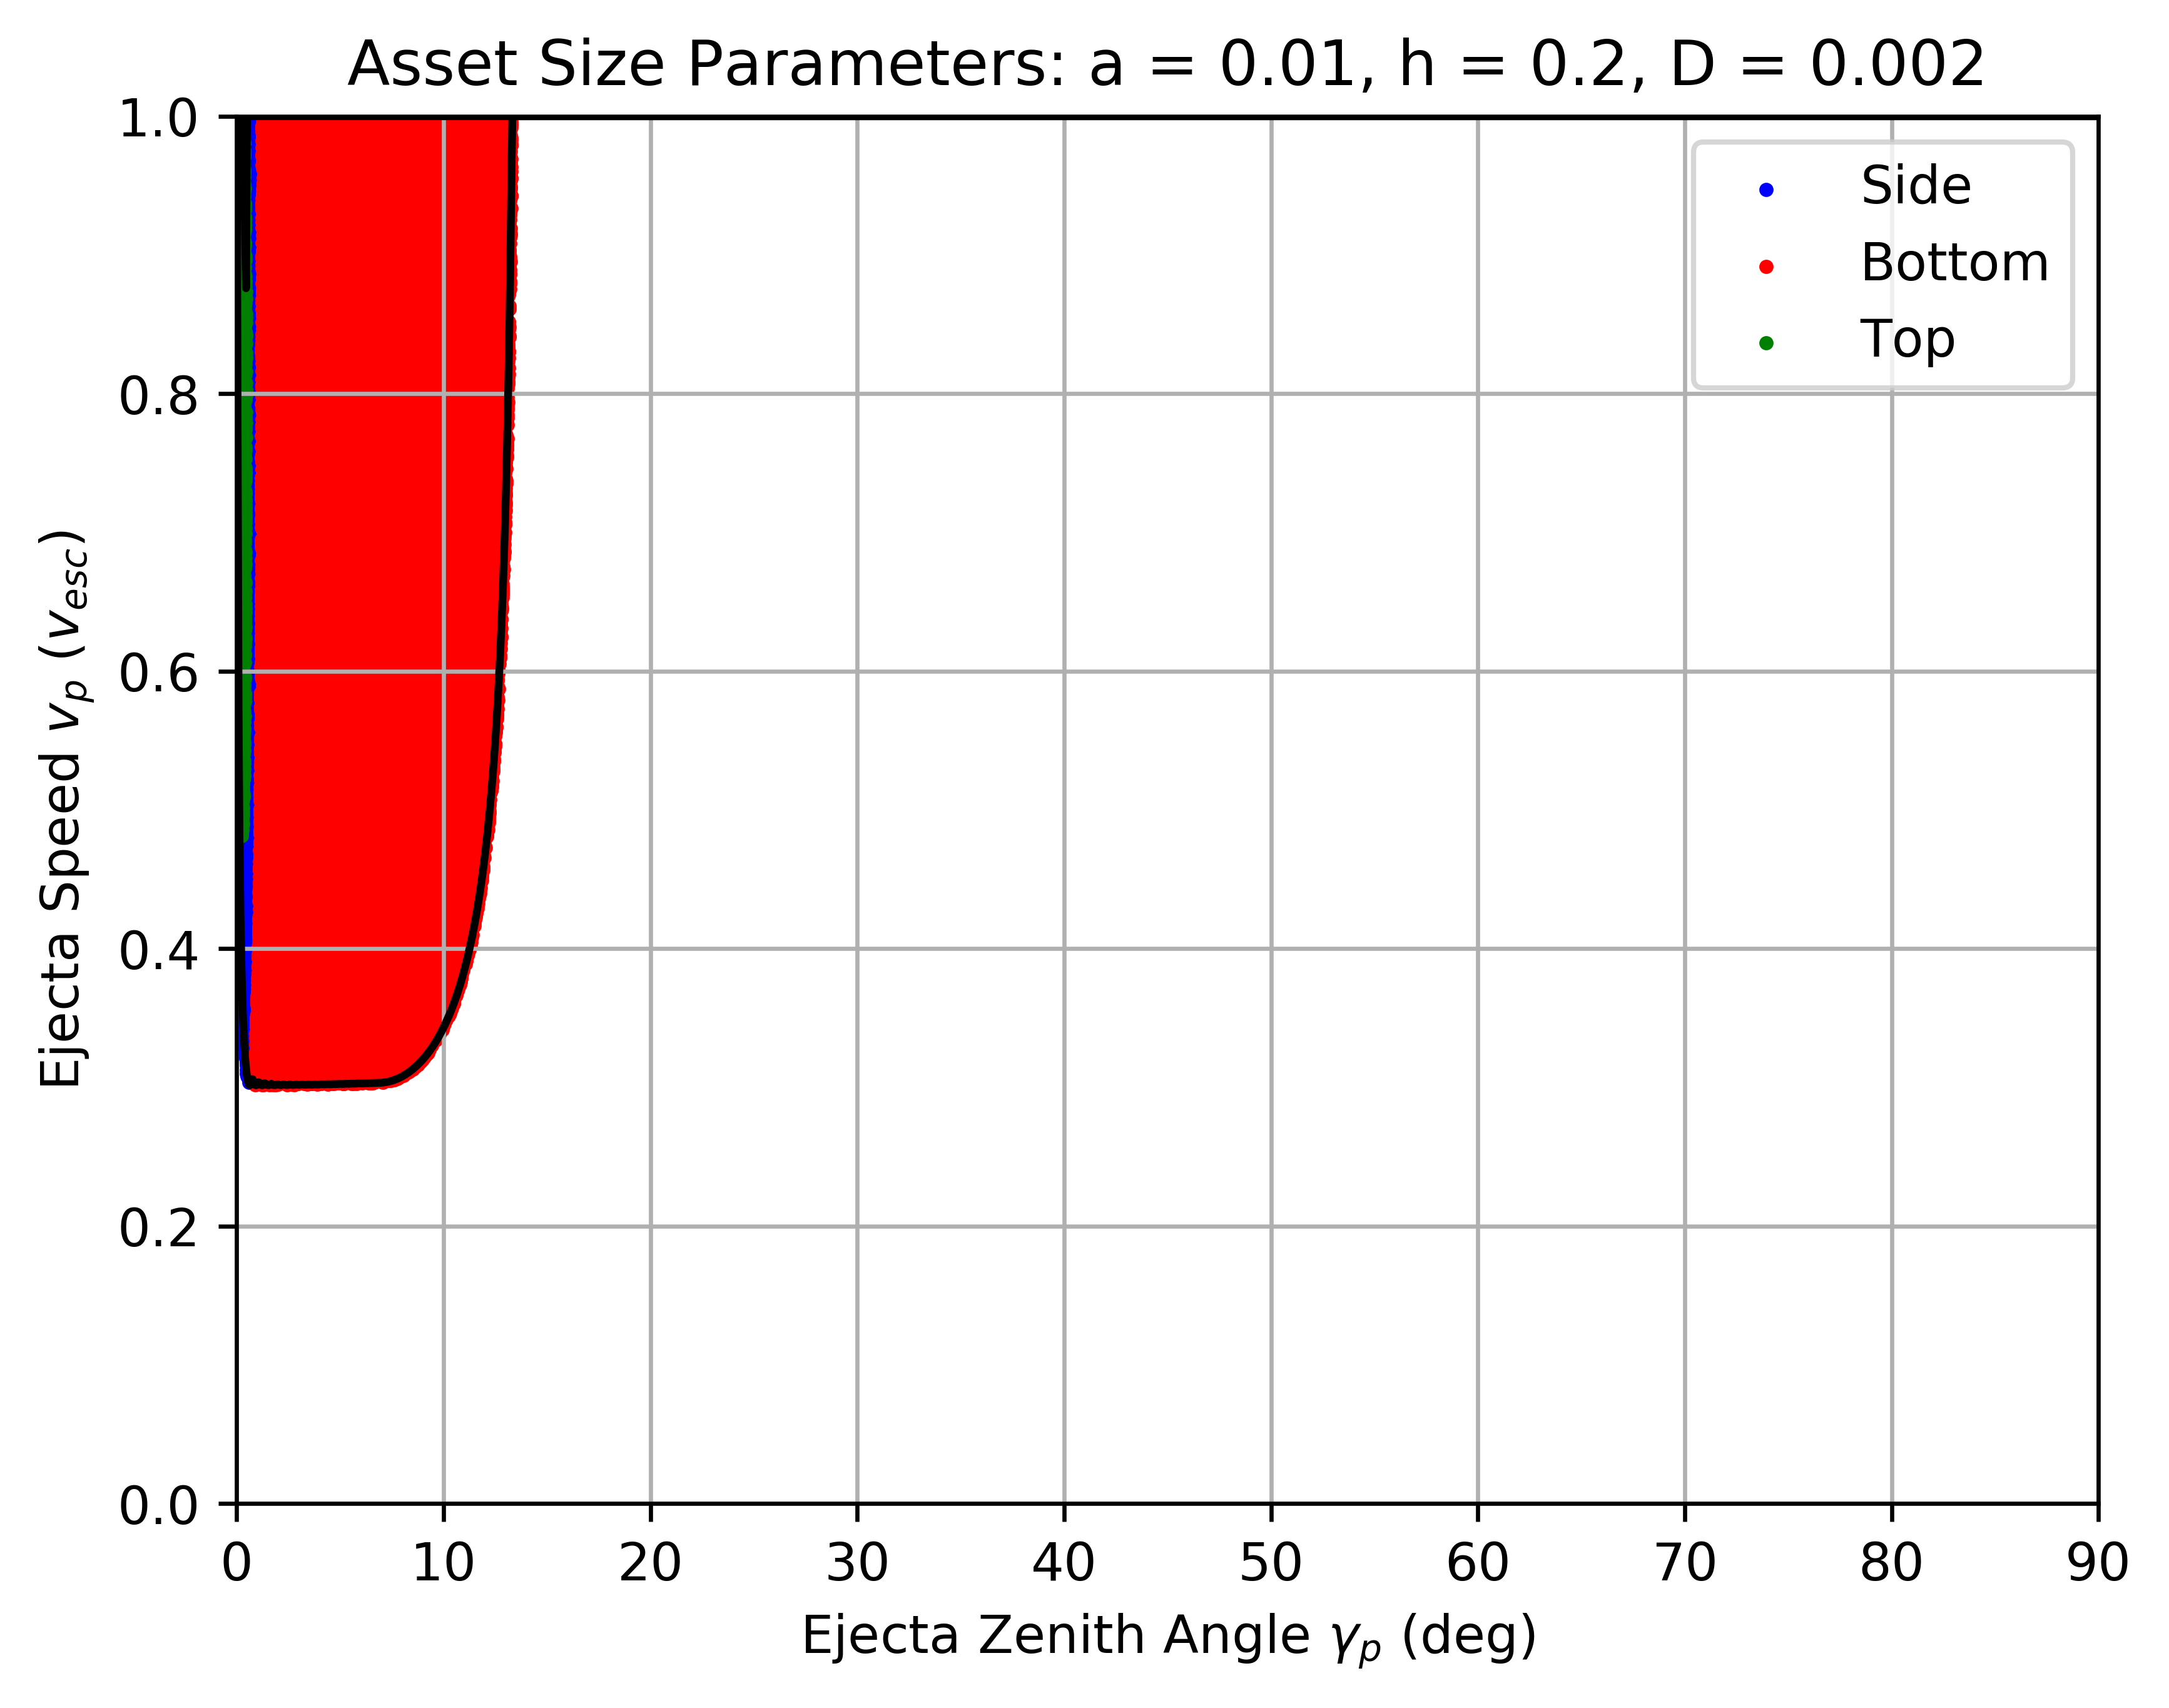
\includegraphics[width=.98\linewidth]{asset_speed_zenith_plot_1.100e+00_1.000e-02_2.000e-01_2.000e-03.png}  
		%\caption{Put your sub-caption here}
		\label{fig:sub-asset_speed_zenith_h2_1}
	\end{subfigure}
	\begin{subfigure}[t]{.32\textwidth}
		\centering
		% include second image
		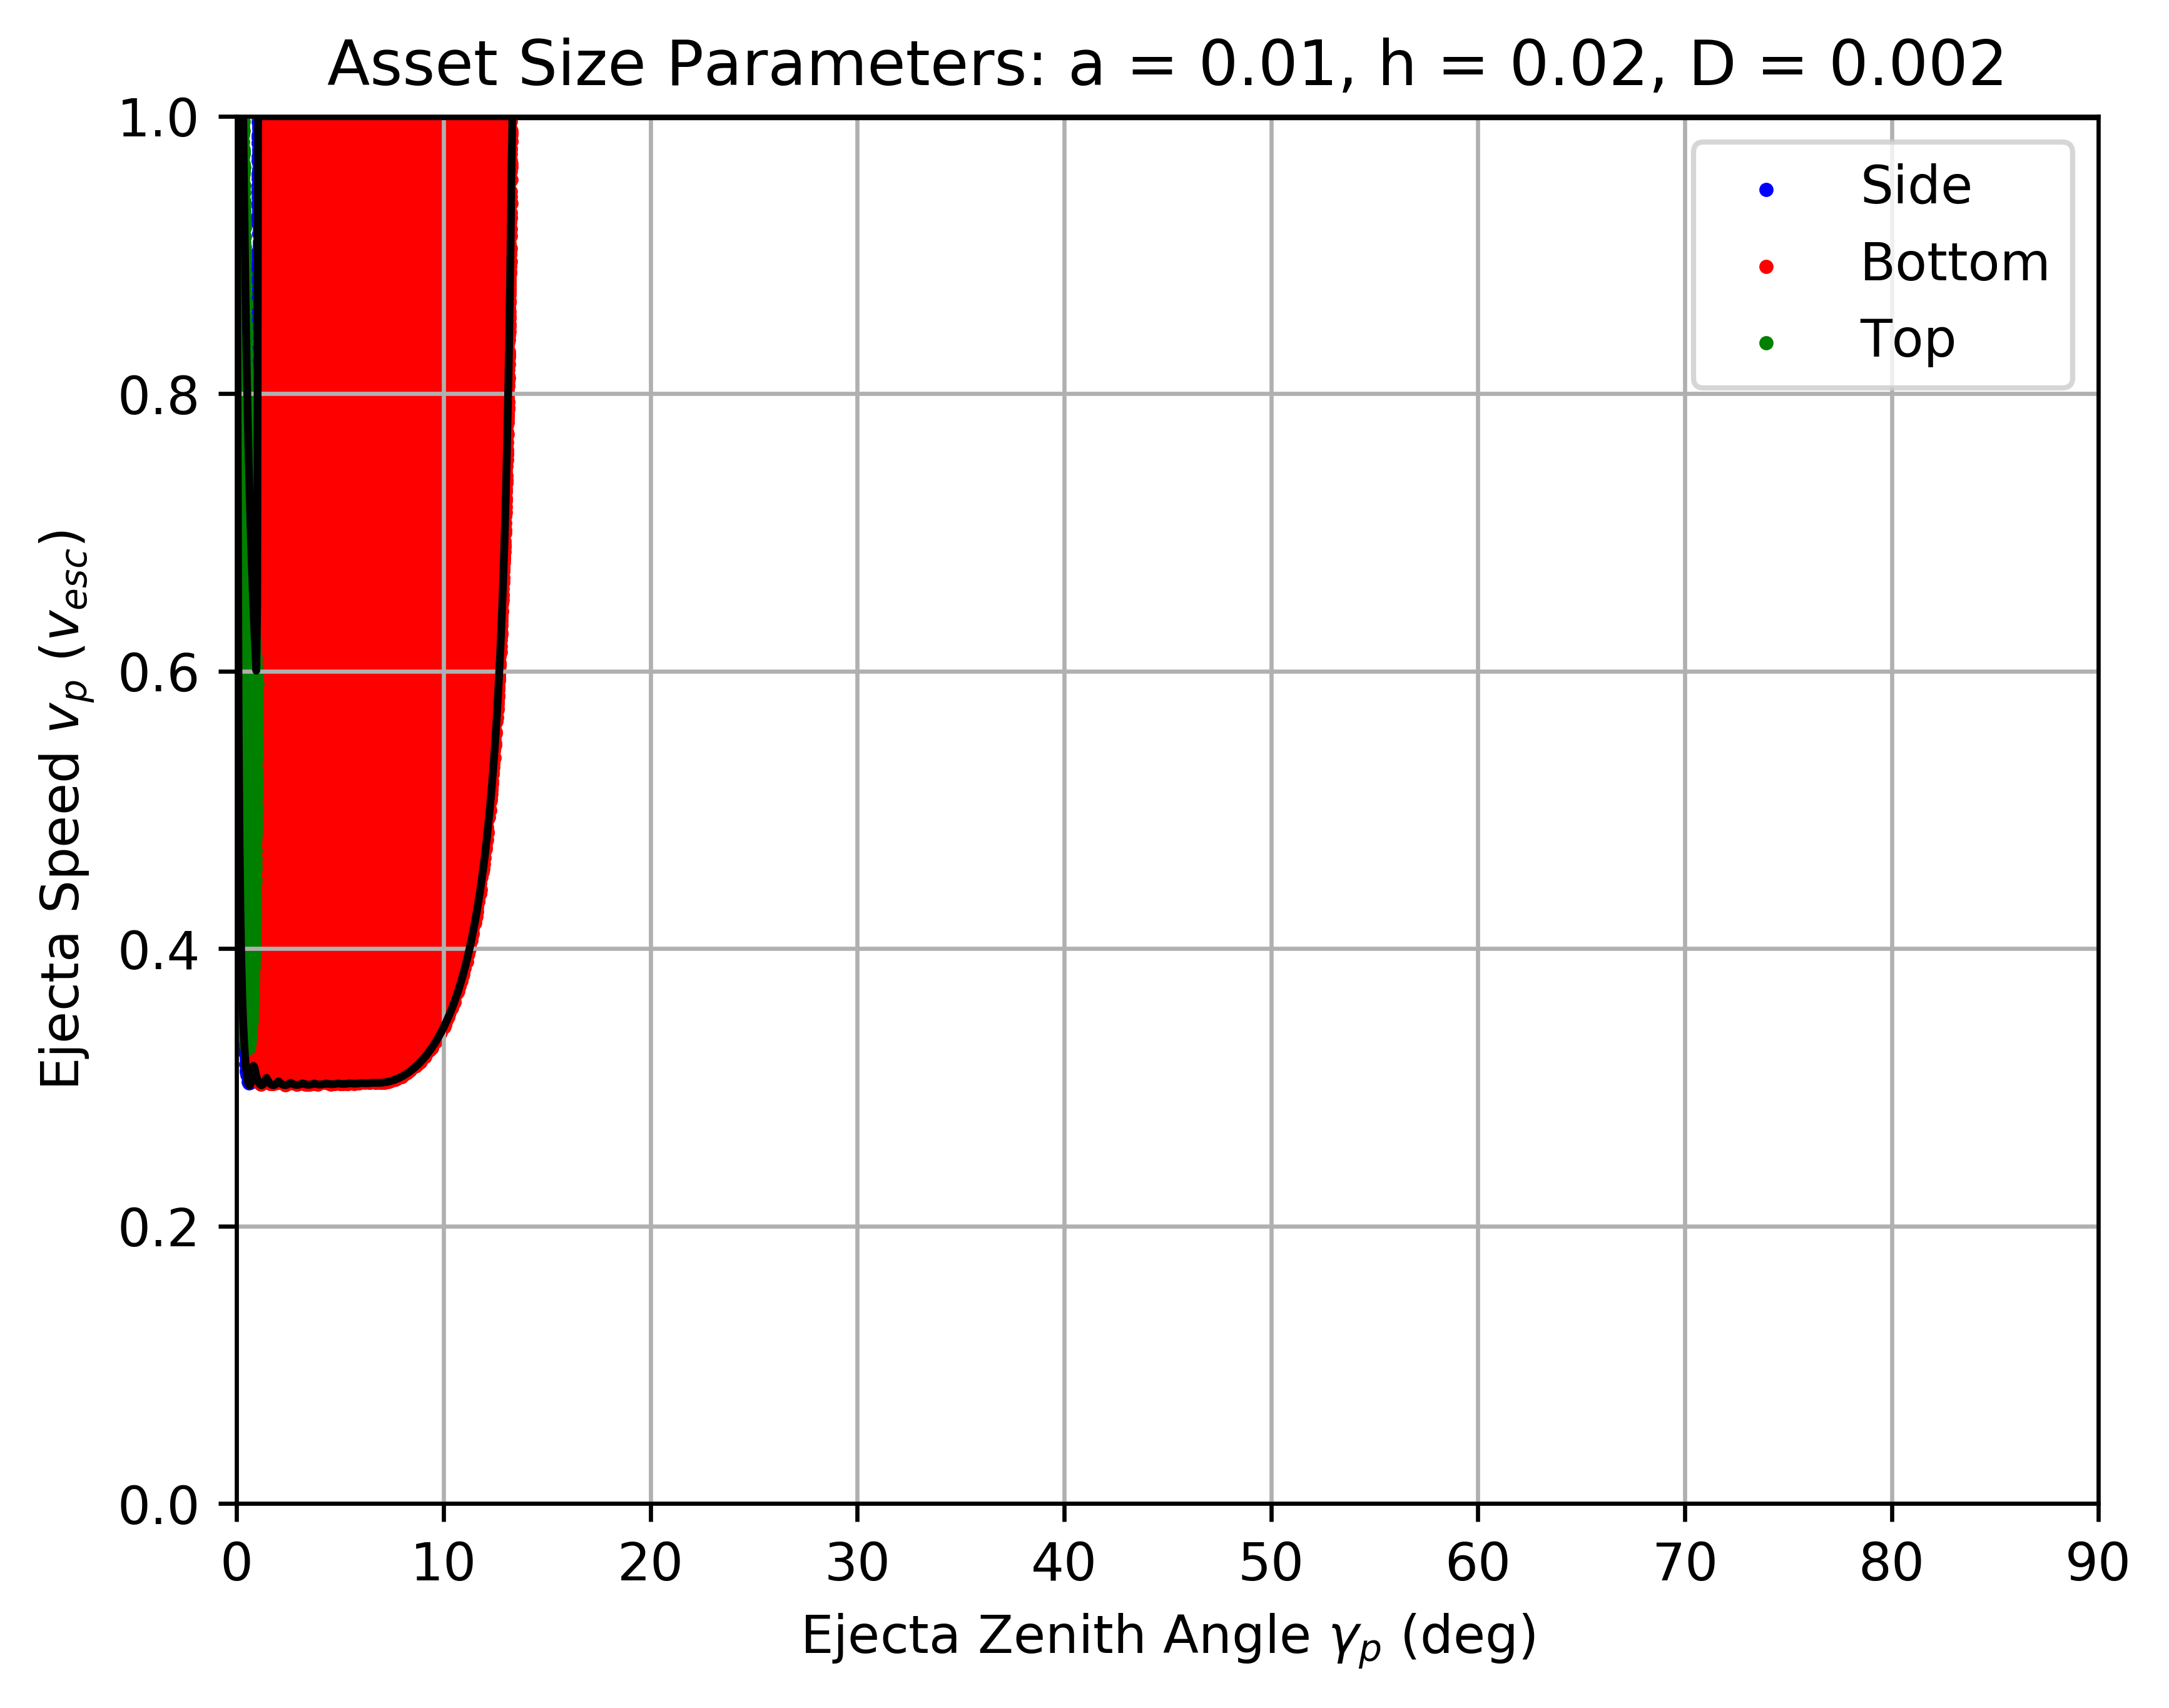
\includegraphics[width=.98\linewidth]{asset_speed_zenith_plot_1.100e+00_1.000e-02_2.000e-02_2.000e-03.png}  
		%\caption{Put your sub-caption here}
		\label{fig:sub-asset_speed_zenith_h2_2}
	\end{subfigure}
	\begin{subfigure}[t]{.32\textwidth}
		\centering
		% include second image
		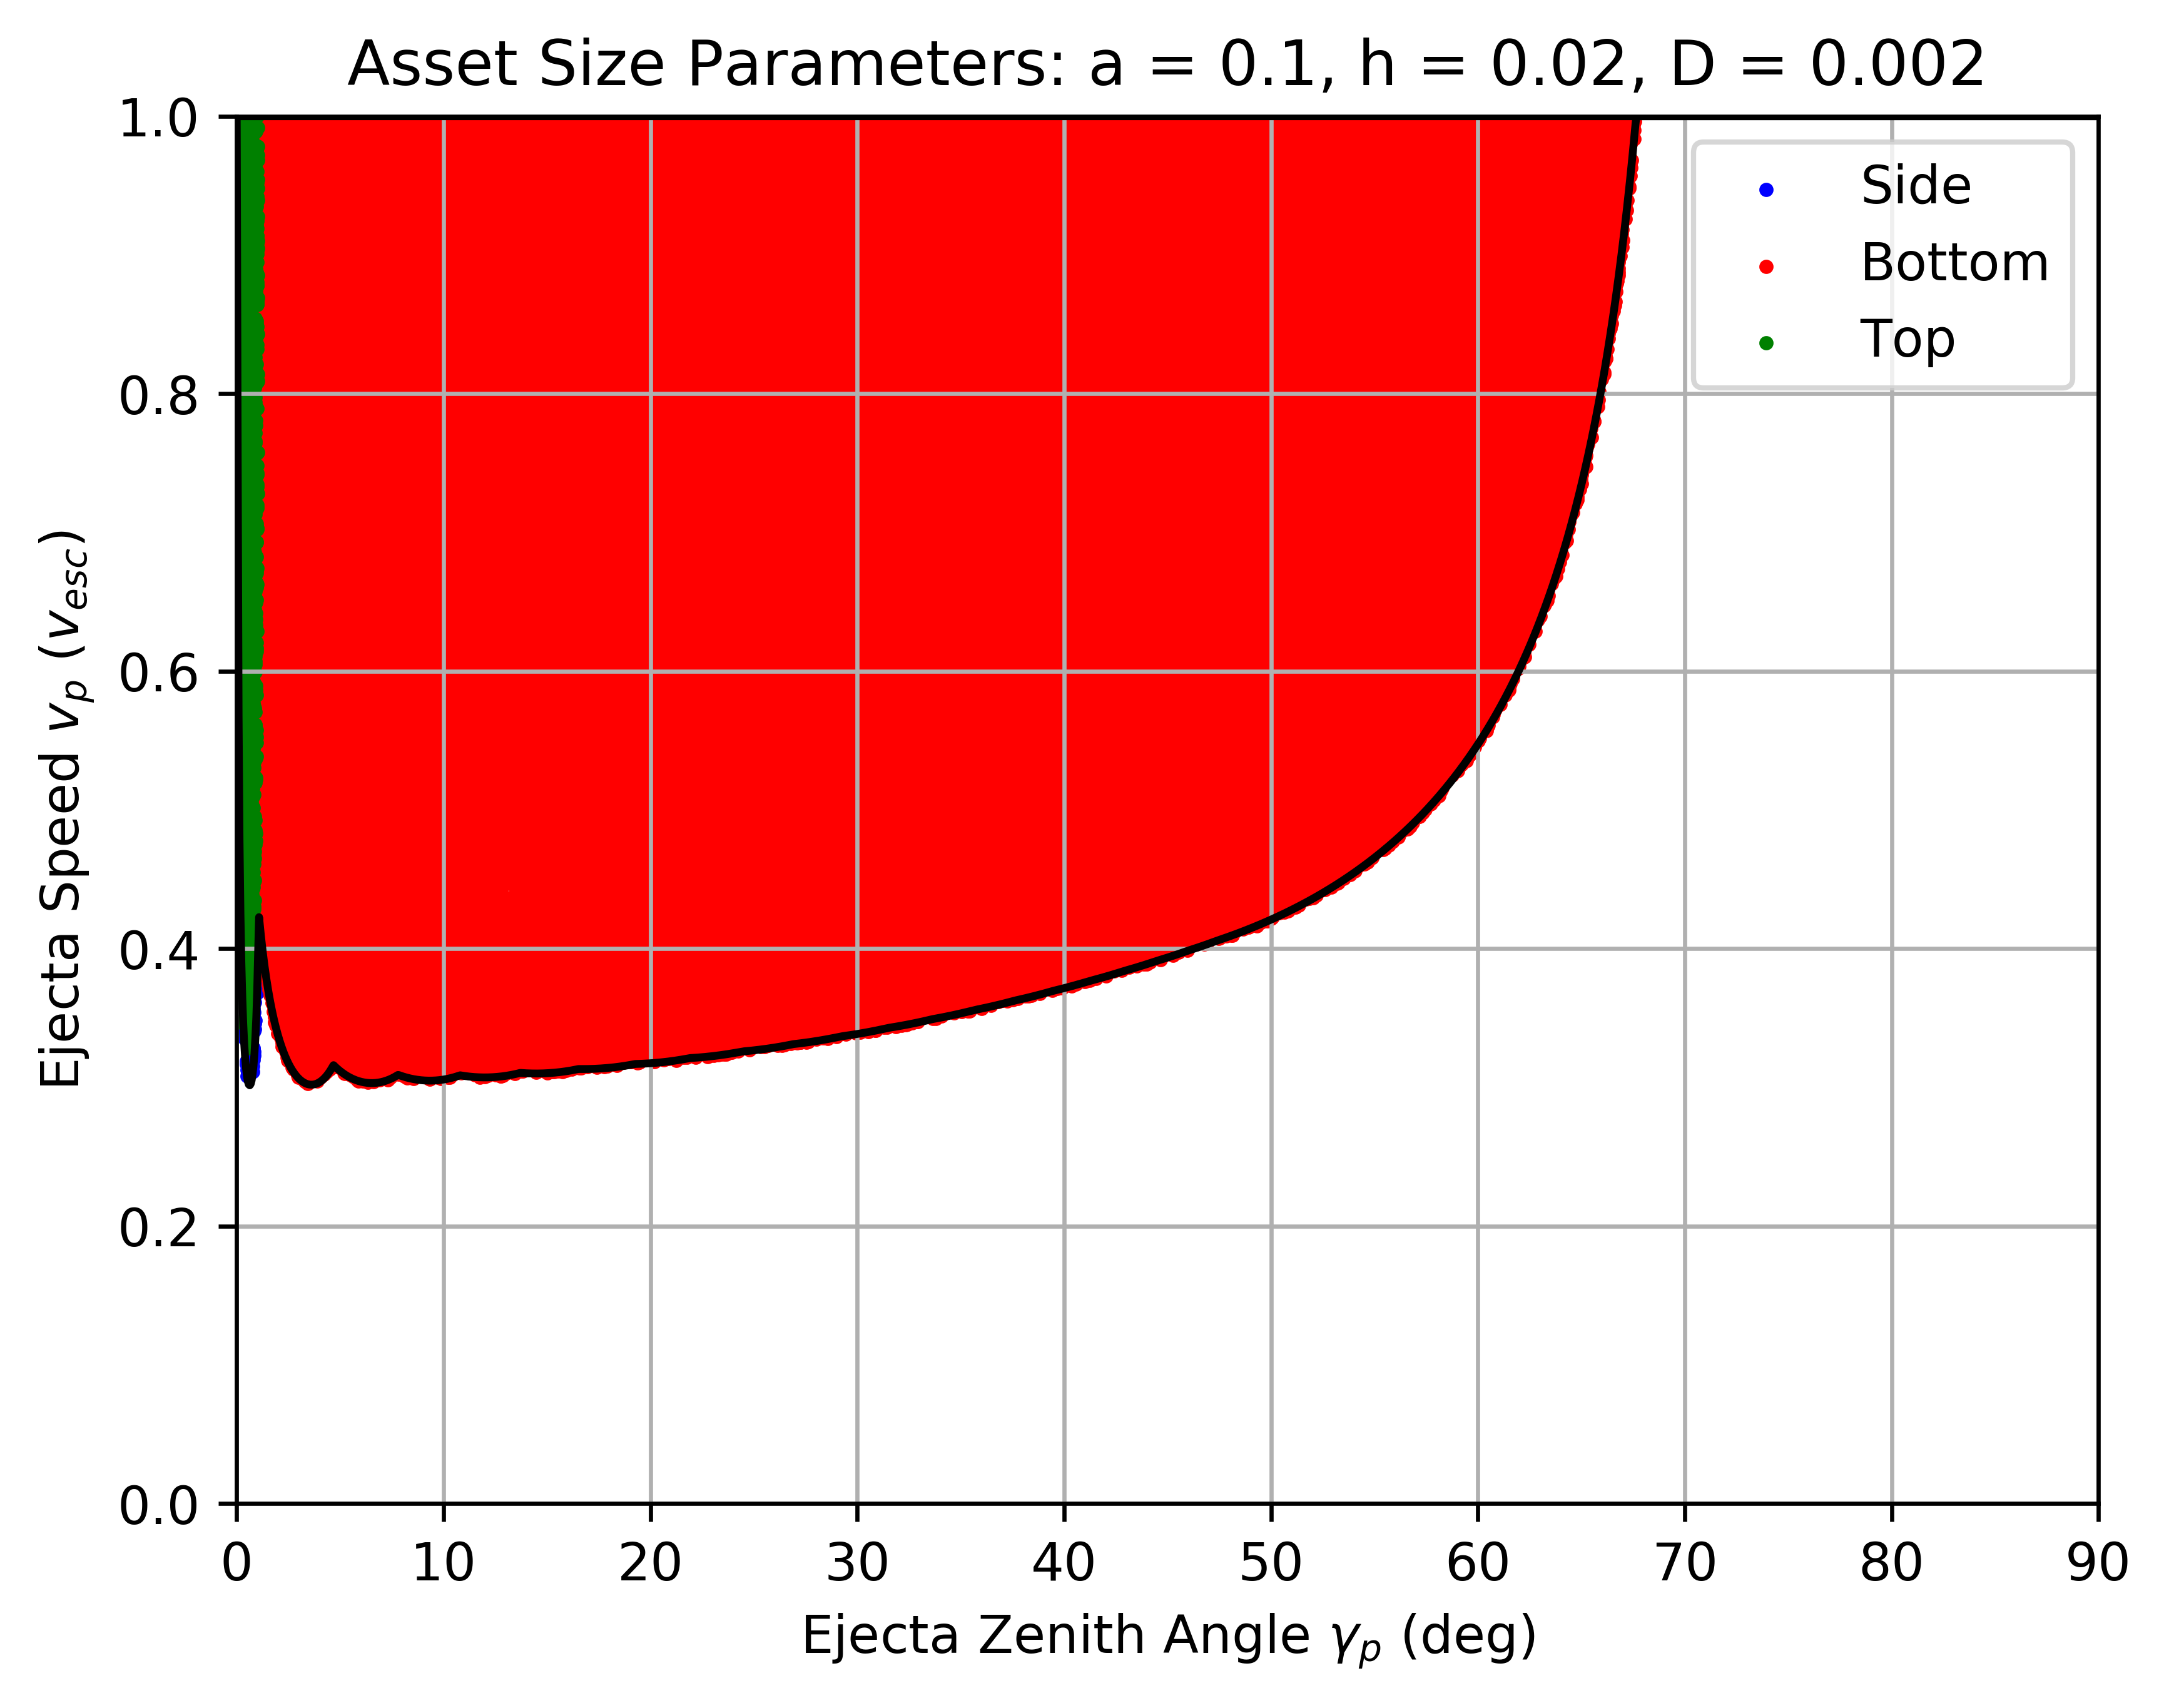
\includegraphics[width=.98\linewidth]{asset_speed_zenith_plot_1.100e+00_1.000e-01_2.000e-02_2.000e-03.png}  
		%\caption{Put your sub-caption here}
		\label{fig:sub-asset_speed_zenith_h2_3}
	\end{subfigure}
	
	%\newline
	
	\begin{subfigure}[t]{.32\textwidth}
		\centering
		% include third image
		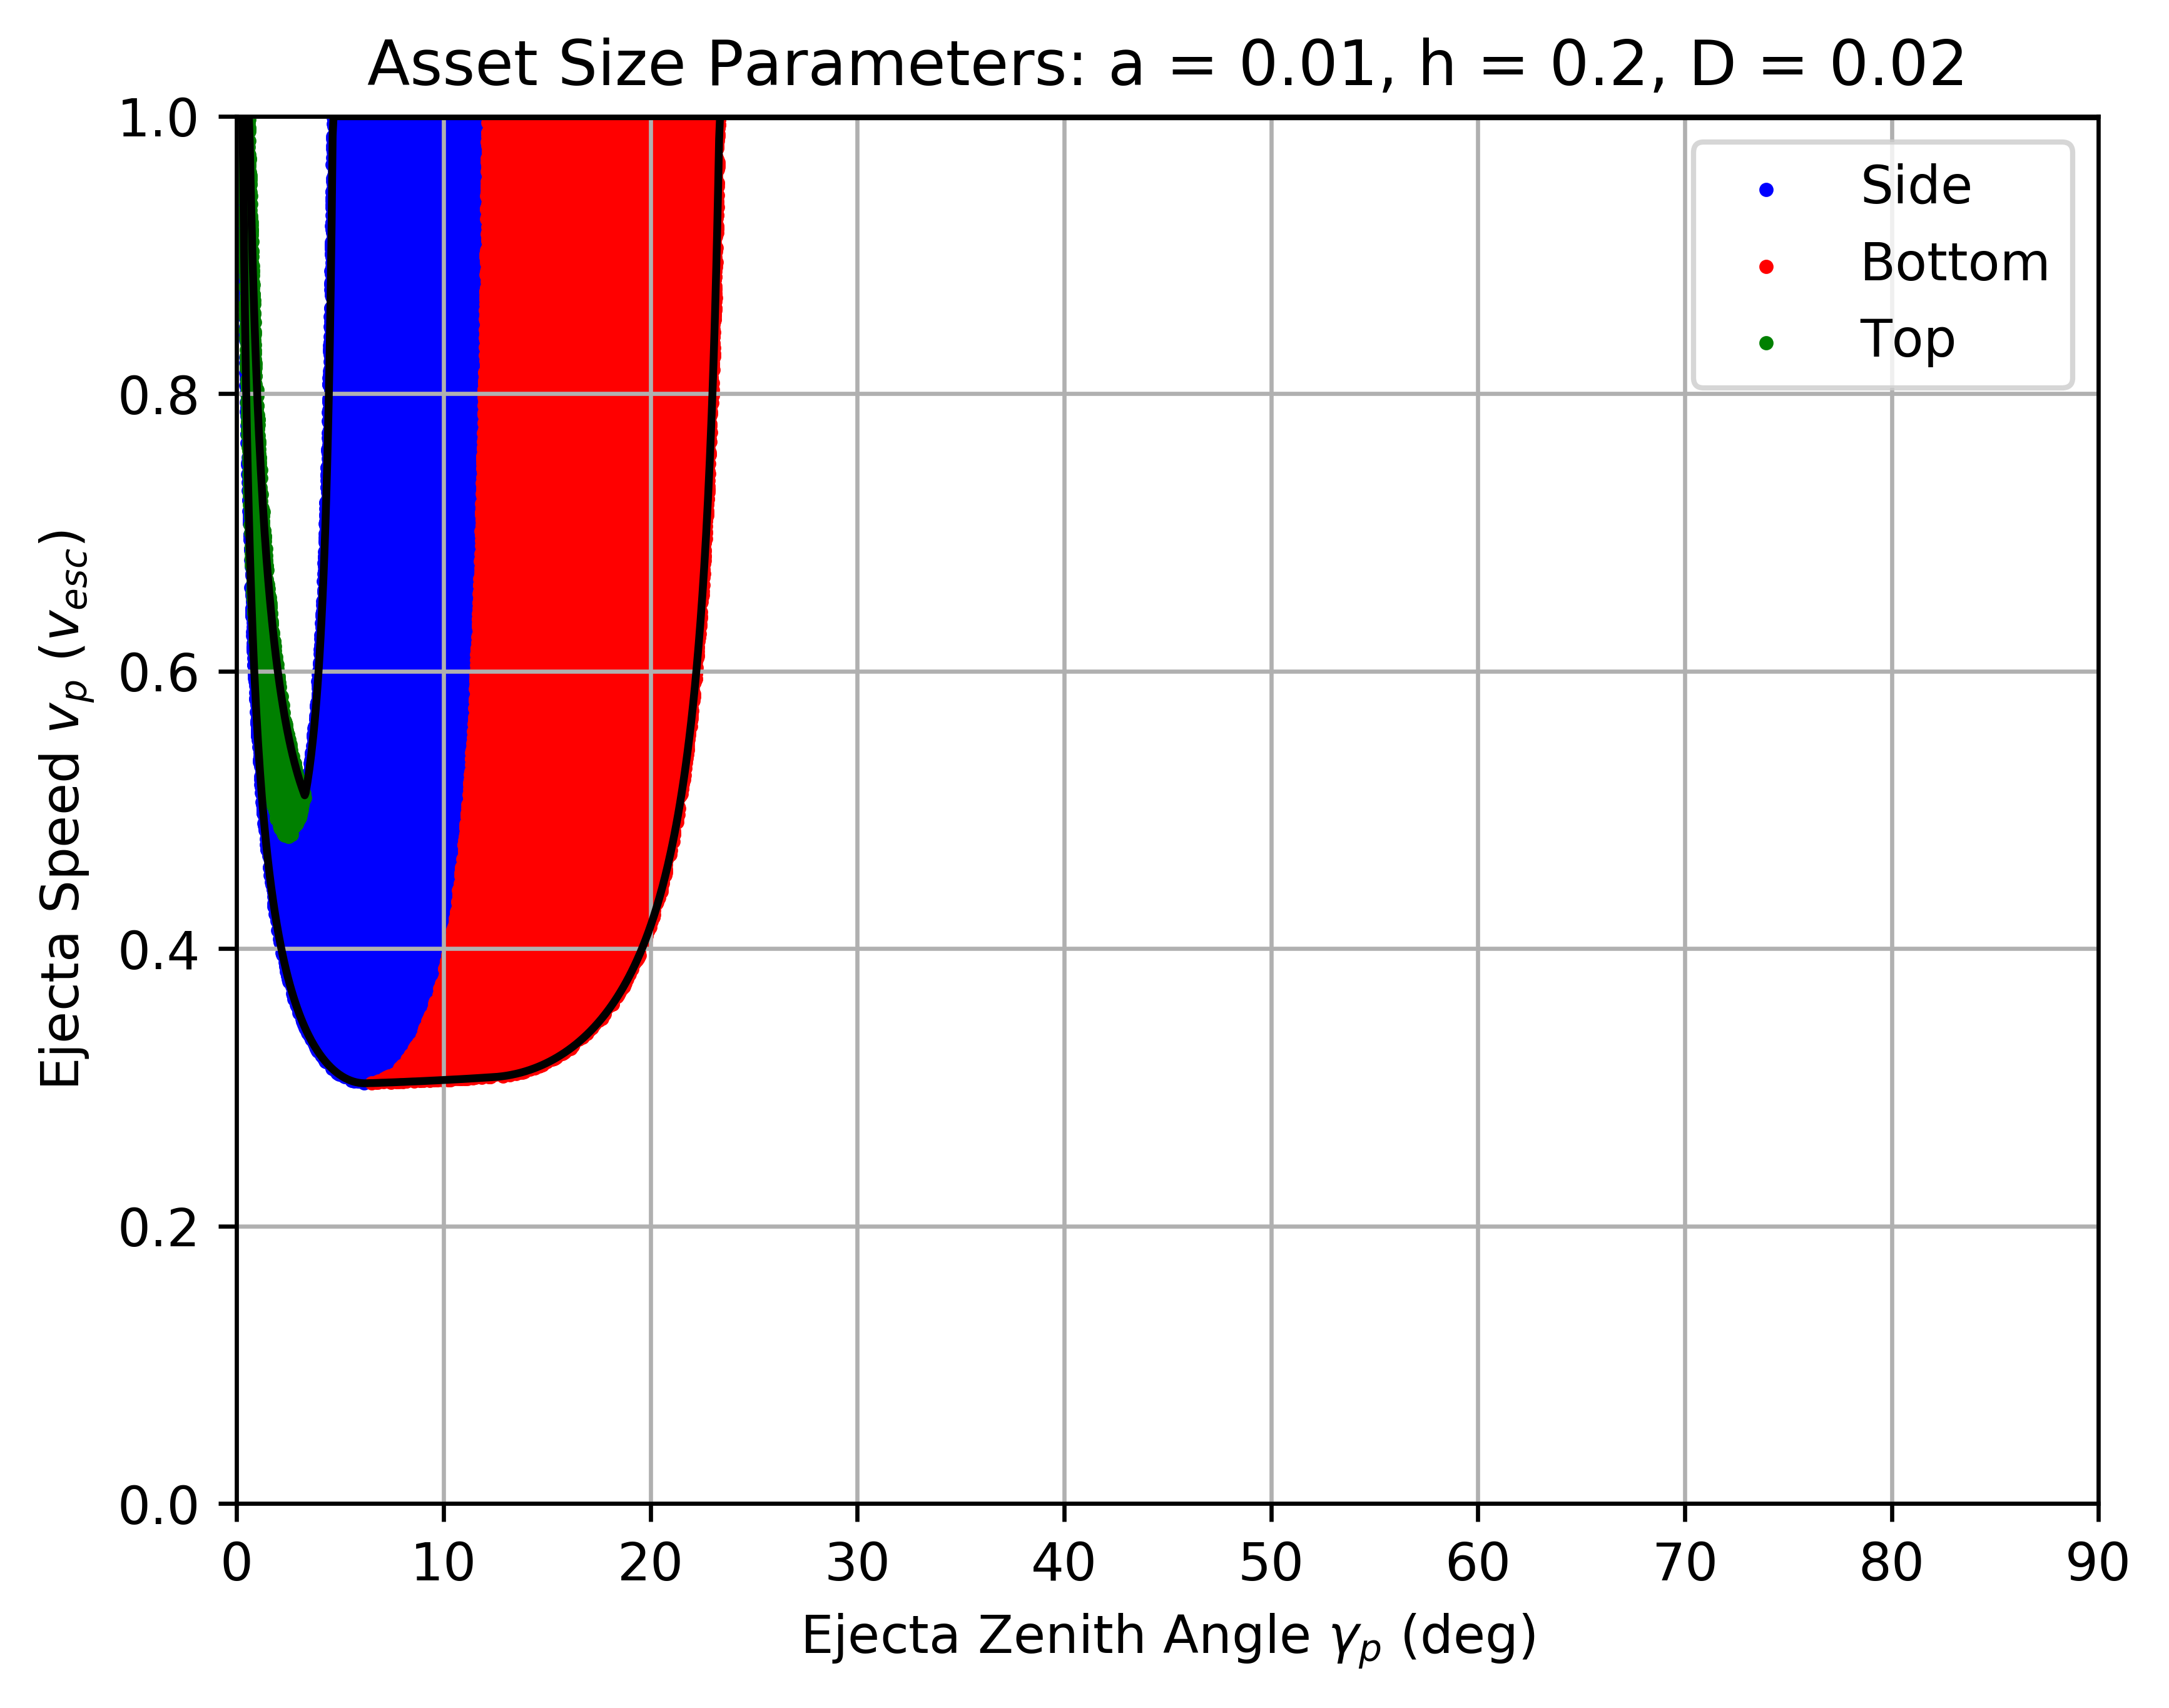
\includegraphics[width=.98\linewidth]{asset_speed_zenith_plot_1.100e+00_1.000e-02_2.000e-01_2.000e-02.png}  
		%\caption{Put your sub-caption here}
		\label{fig:sub-asset_speed_zenith_h2_4}
	\end{subfigure}
	\begin{subfigure}[t]{.32\textwidth}
		\centering
		% include fourth image
		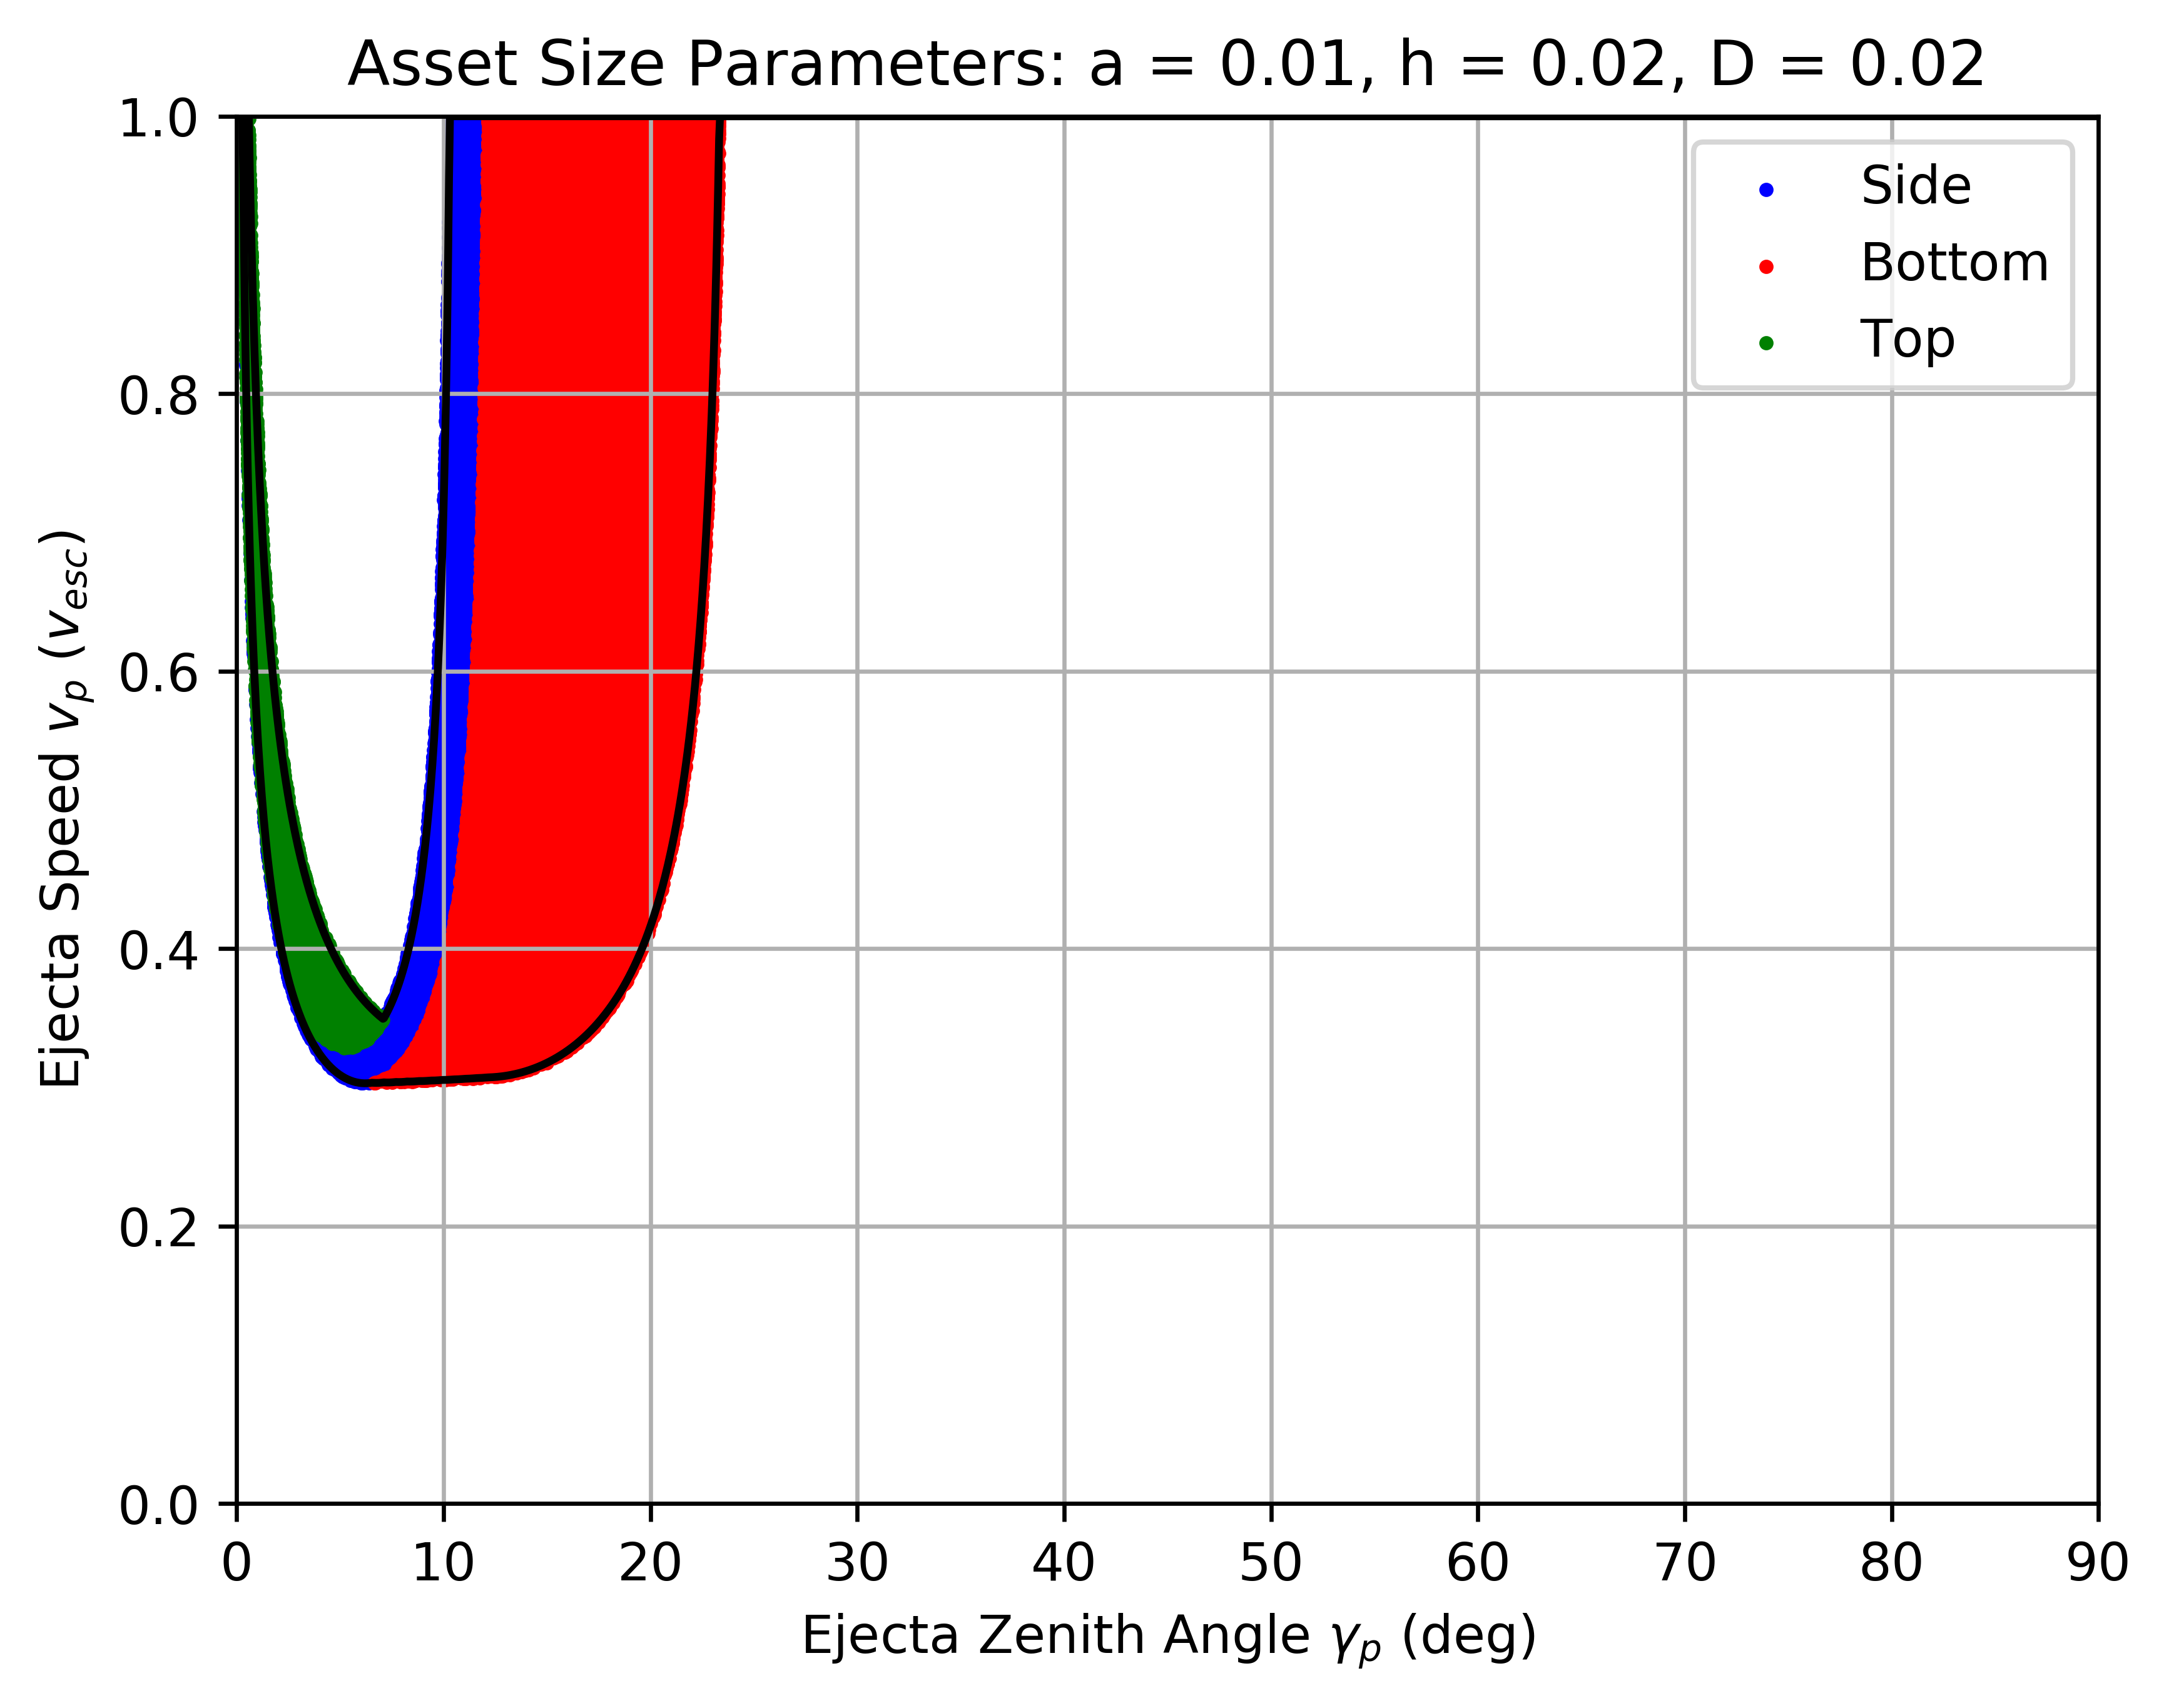
\includegraphics[width=.98\linewidth]{asset_speed_zenith_plot_1.100e+00_1.000e-02_2.000e-02_2.000e-02.png}  
		%\caption{Put your sub-caption here}
		\label{fig:sub-asset_speed_zenith_h2_5}
	\end{subfigure}
	\begin{subfigure}[t]{.32\textwidth}
		\centering
		% include fourth image
		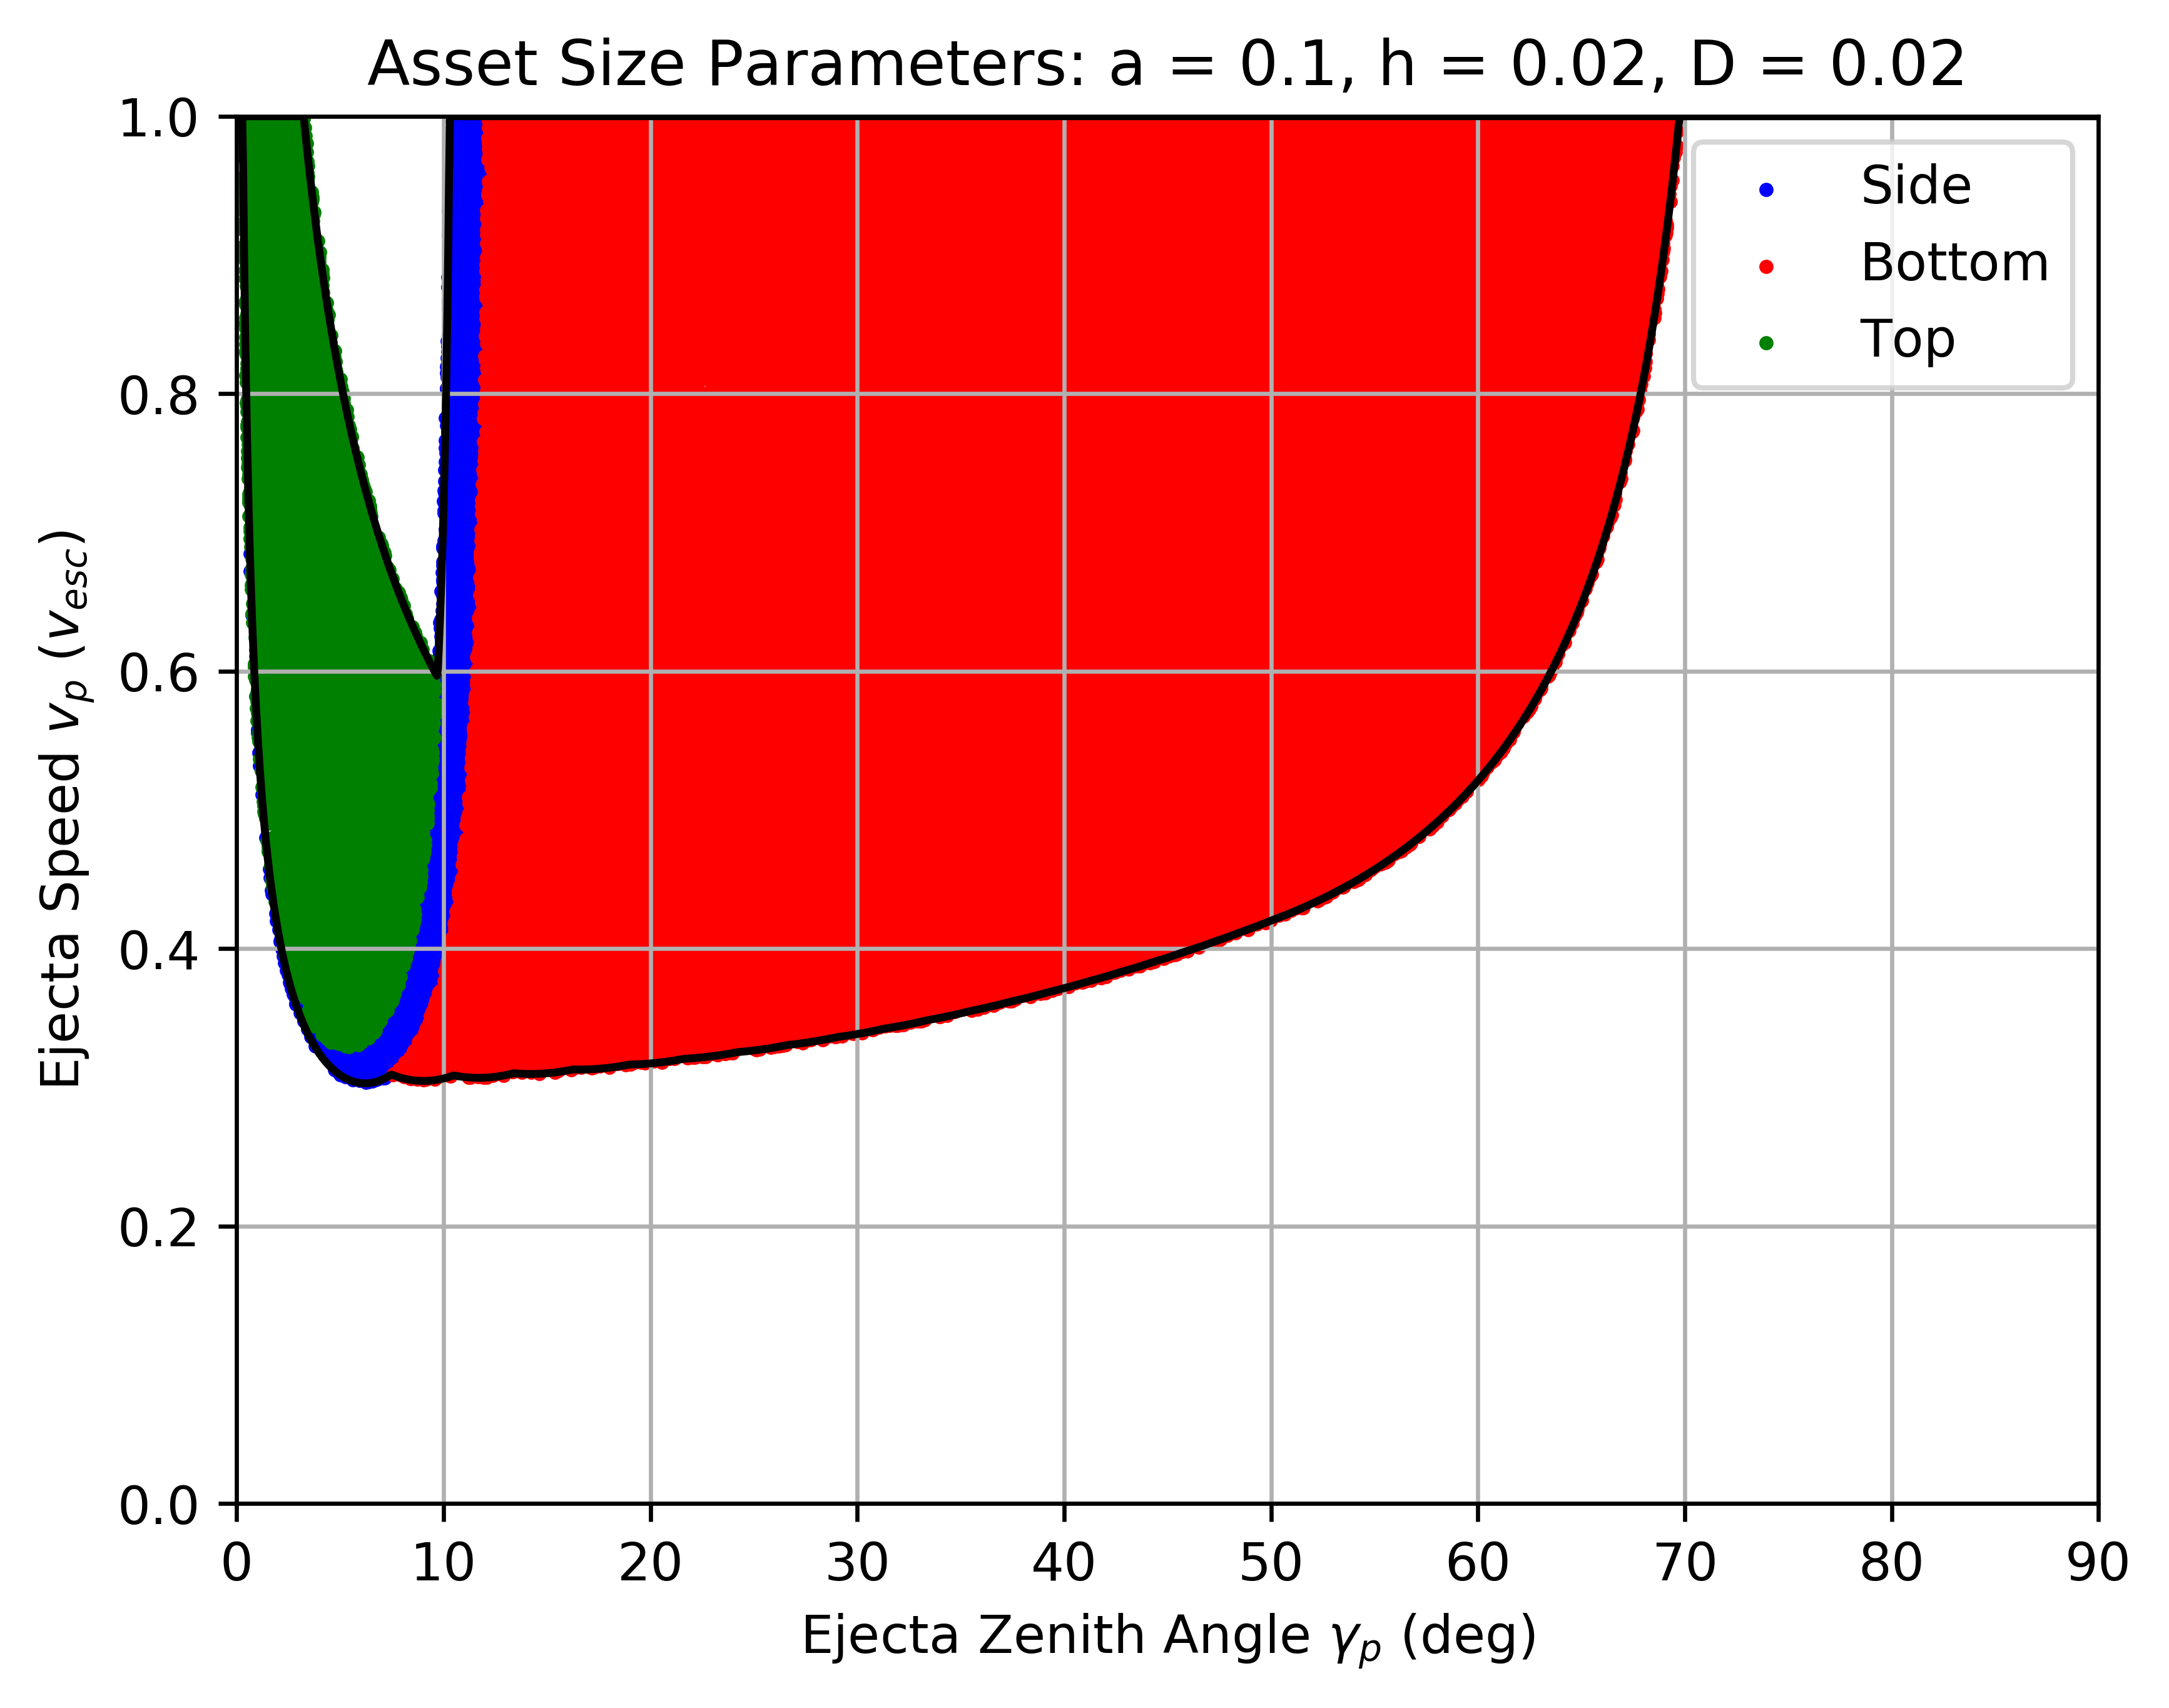
\includegraphics[width=.98\linewidth]{asset_speed_zenith_plot_1.100e+00_1.000e-01_2.000e-02_2.000e-02.png}  
		%\caption{Put your sub-caption here}
		\label{fig:sub-asset_speed_zenith_h2_6}
	\end{subfigure}
	
	
	\begin{subfigure}[t]{.32\textwidth}
		\centering
		% include third image
		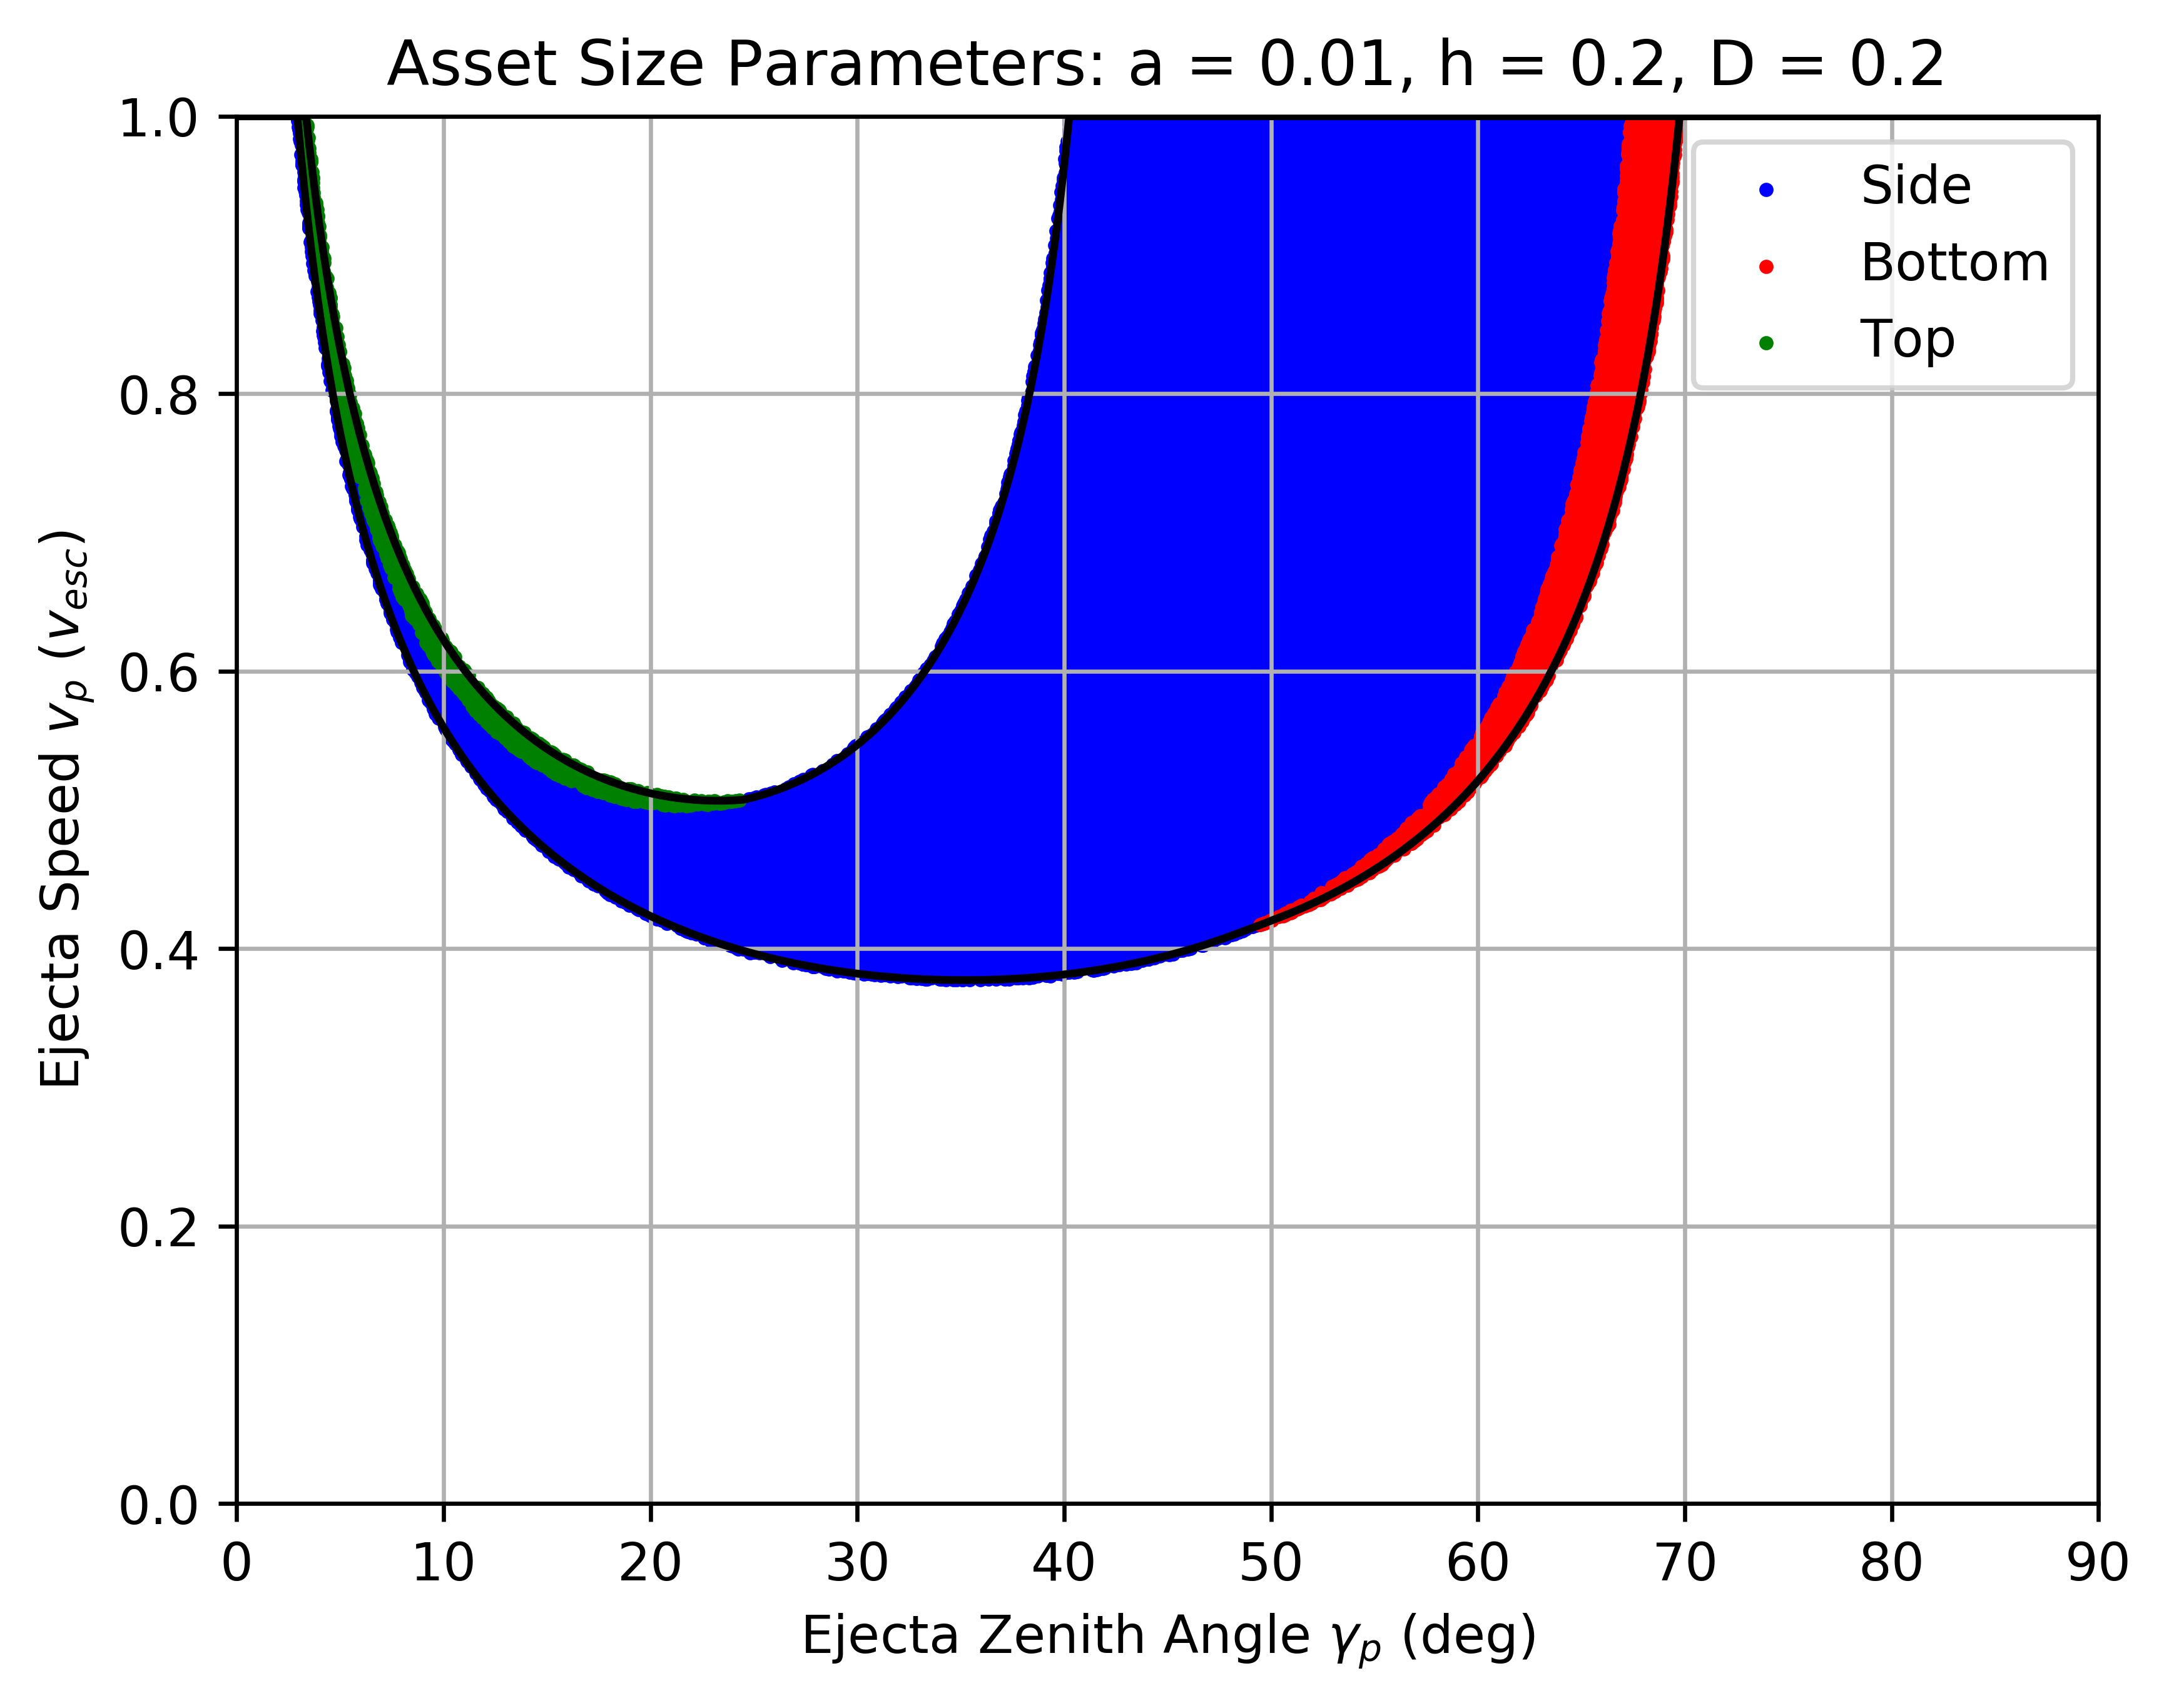
\includegraphics[width=.98\linewidth]{asset_speed_zenith_plot_1.100e+00_1.000e-02_2.000e-01_2.000e-01.png}  
		%\caption{Put your sub-caption here}
		\label{fig:sub-asset_speed_zenith_h2_7}
	\end{subfigure}
	\begin{subfigure}[t]{.32\textwidth}
		\centering
		% include fourth image
		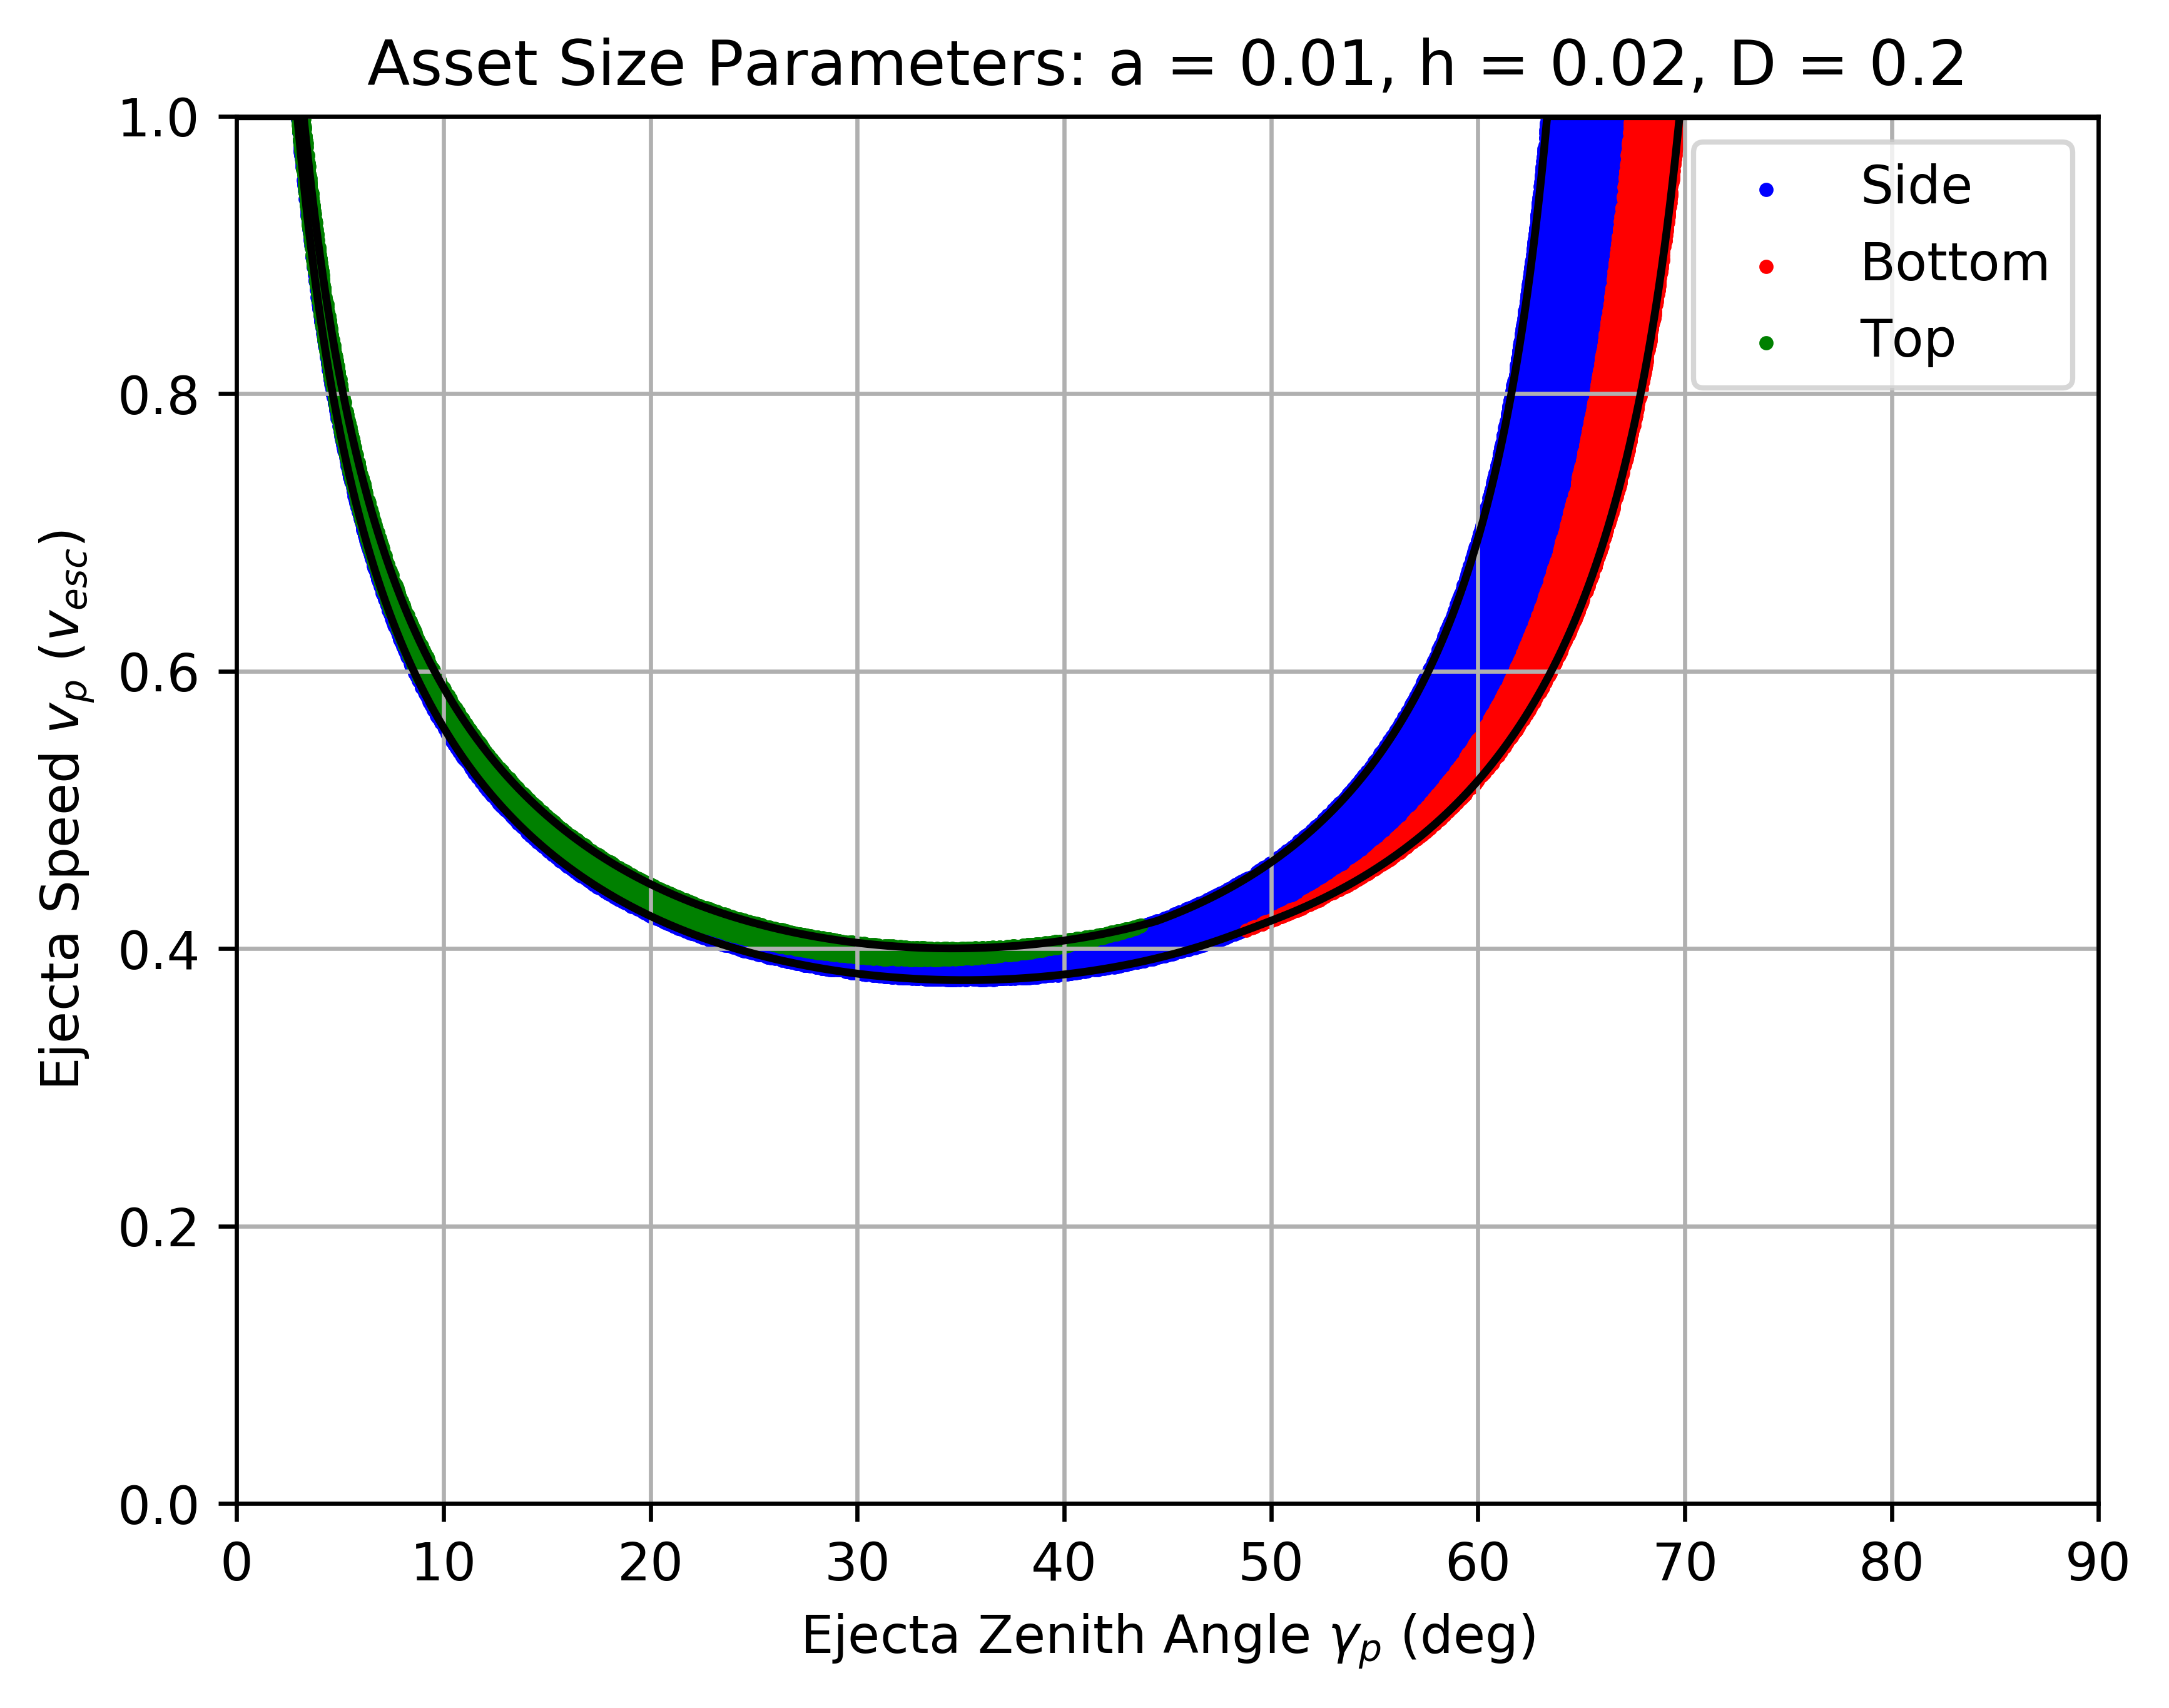
\includegraphics[width=.98\linewidth]{asset_speed_zenith_plot_1.100e+00_1.000e-02_2.000e-02_2.000e-01.png}  
		%\caption{Put your sub-caption here}
		\label{fig:sub-asset_speed_zenith_h2_8}
	\end{subfigure}
	\begin{subfigure}[t]{.32\textwidth}
		\centering
		% include fourth image
		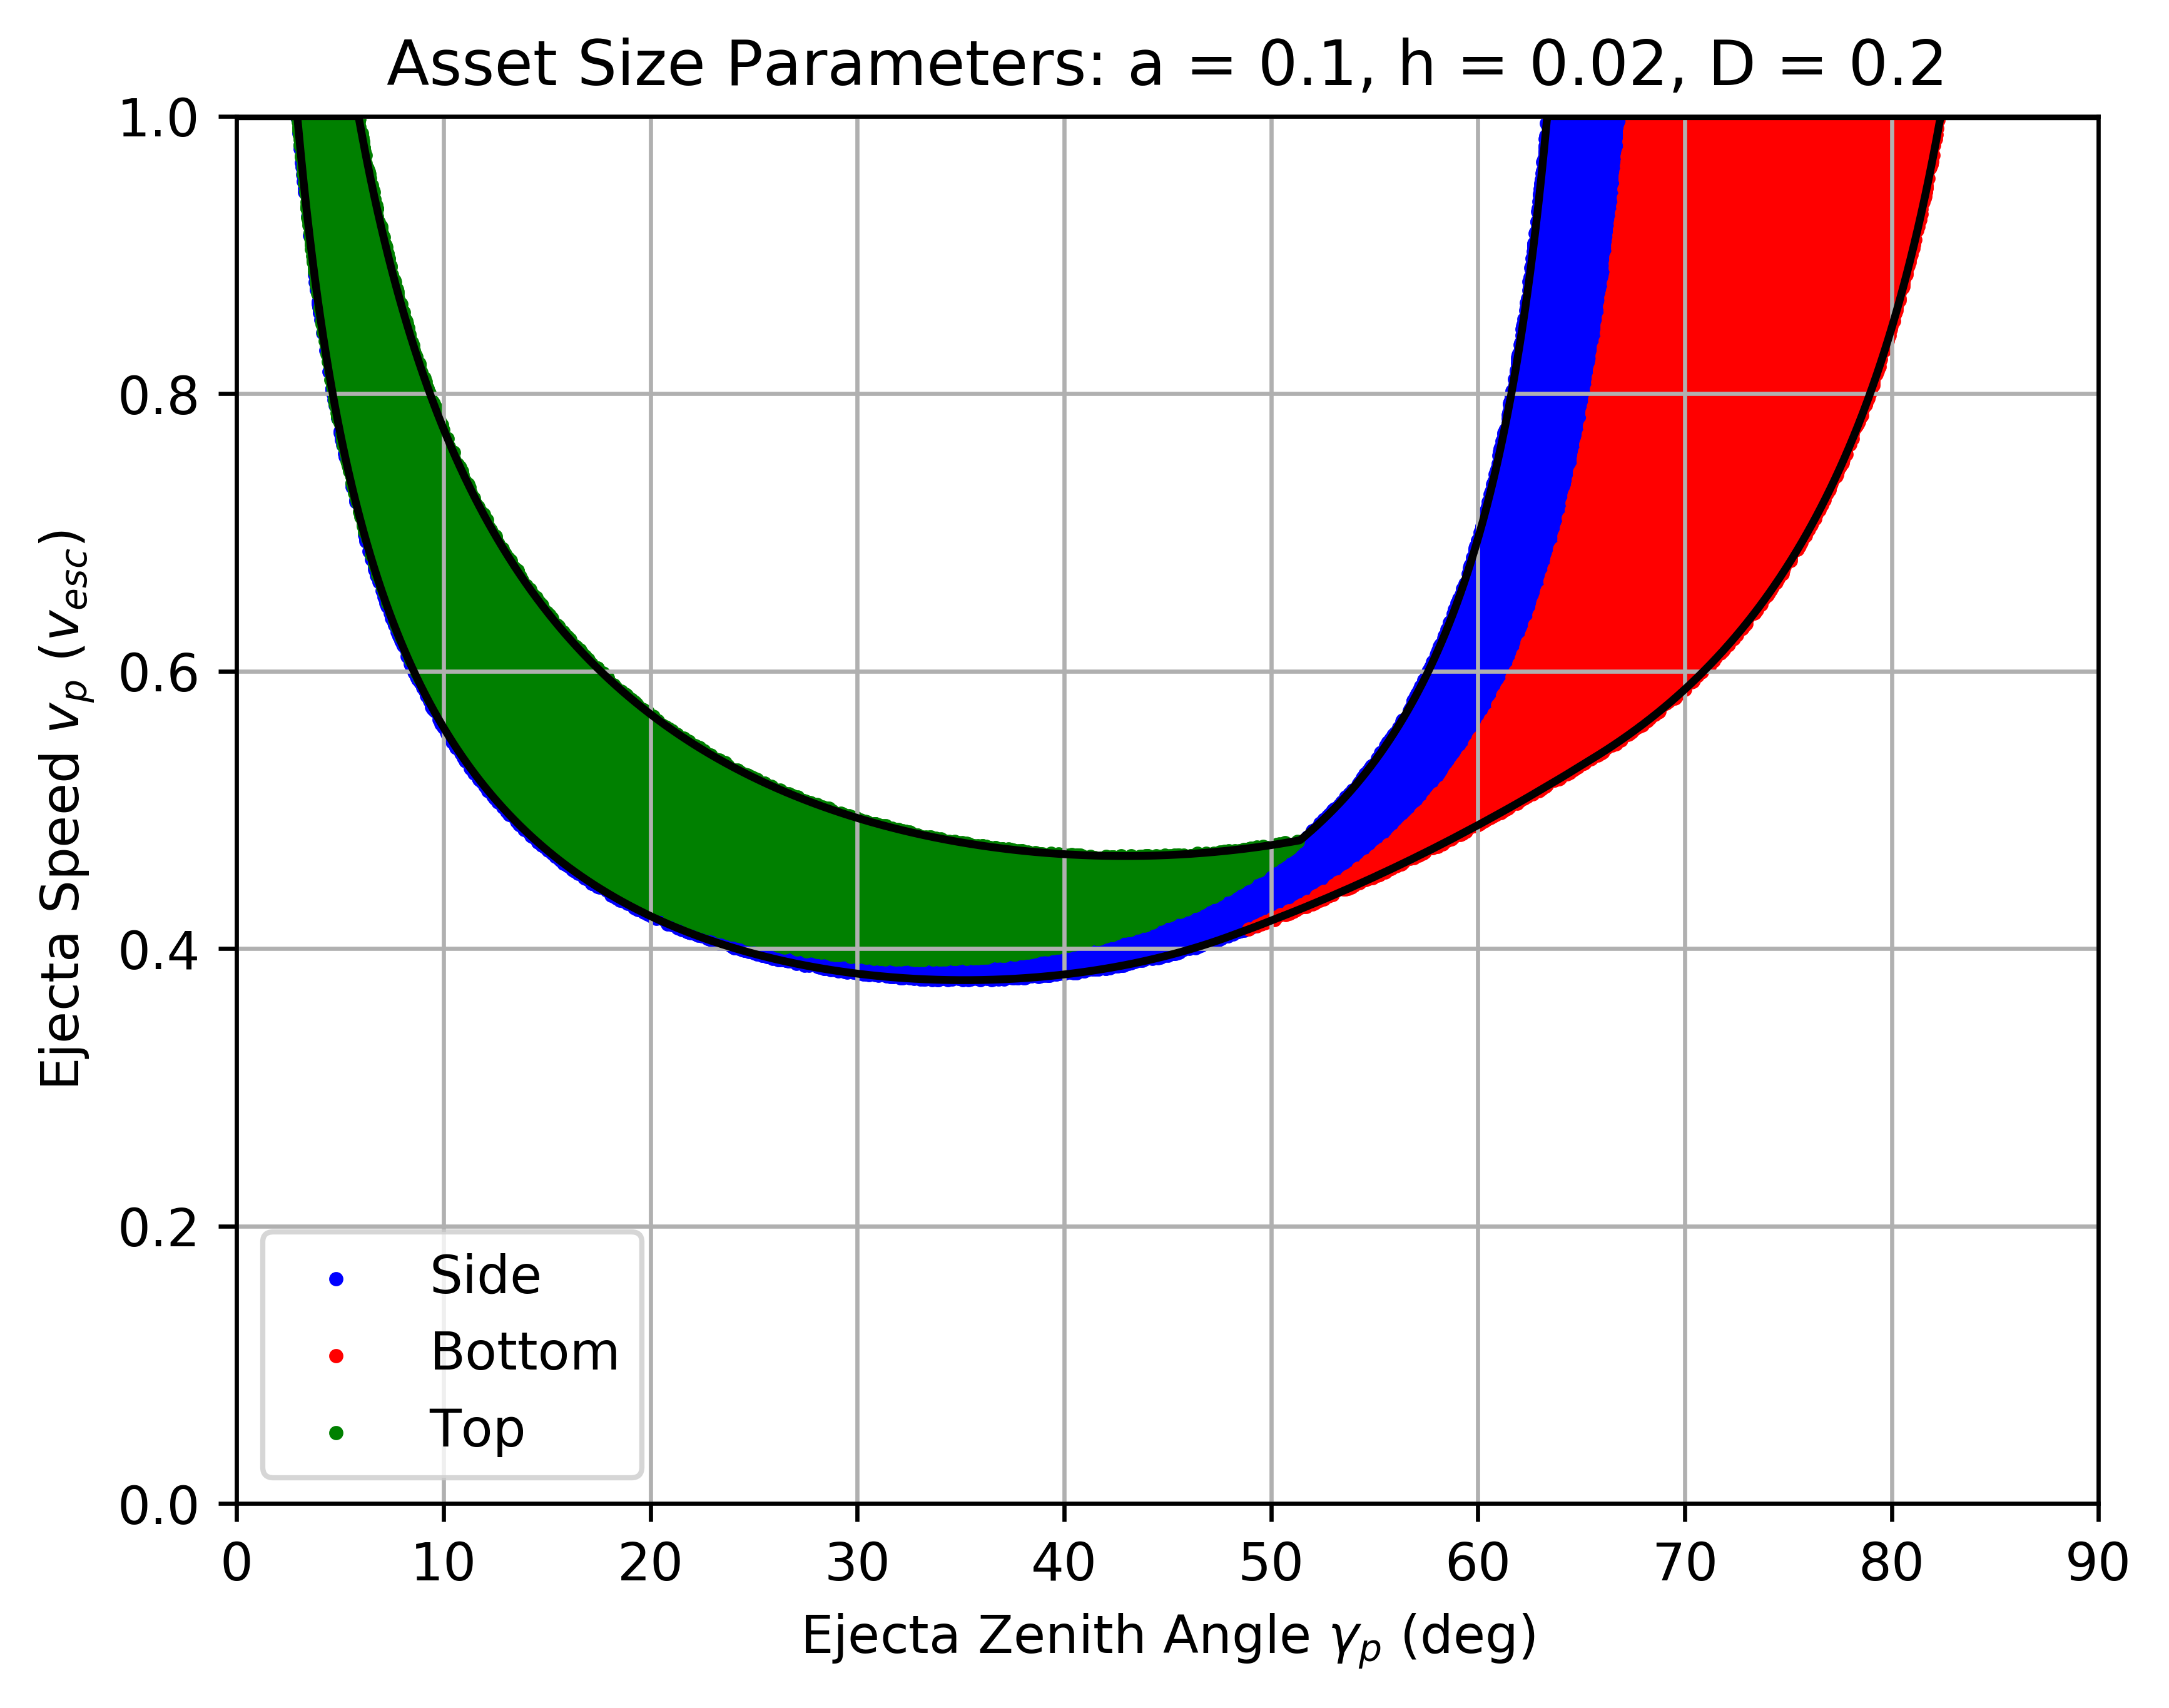
\includegraphics[width=.98\linewidth]{asset_speed_zenith_plot_1.100e+00_1.000e-01_2.000e-02_2.000e-01.png}  
		%\caption{Put your sub-caption here}
		\label{fig:sub-asset_speed_zenith_h2_9}
	\end{subfigure}
	
	\begin{subfigure}[t]{.32\textwidth}
		\centering
		% include third image
		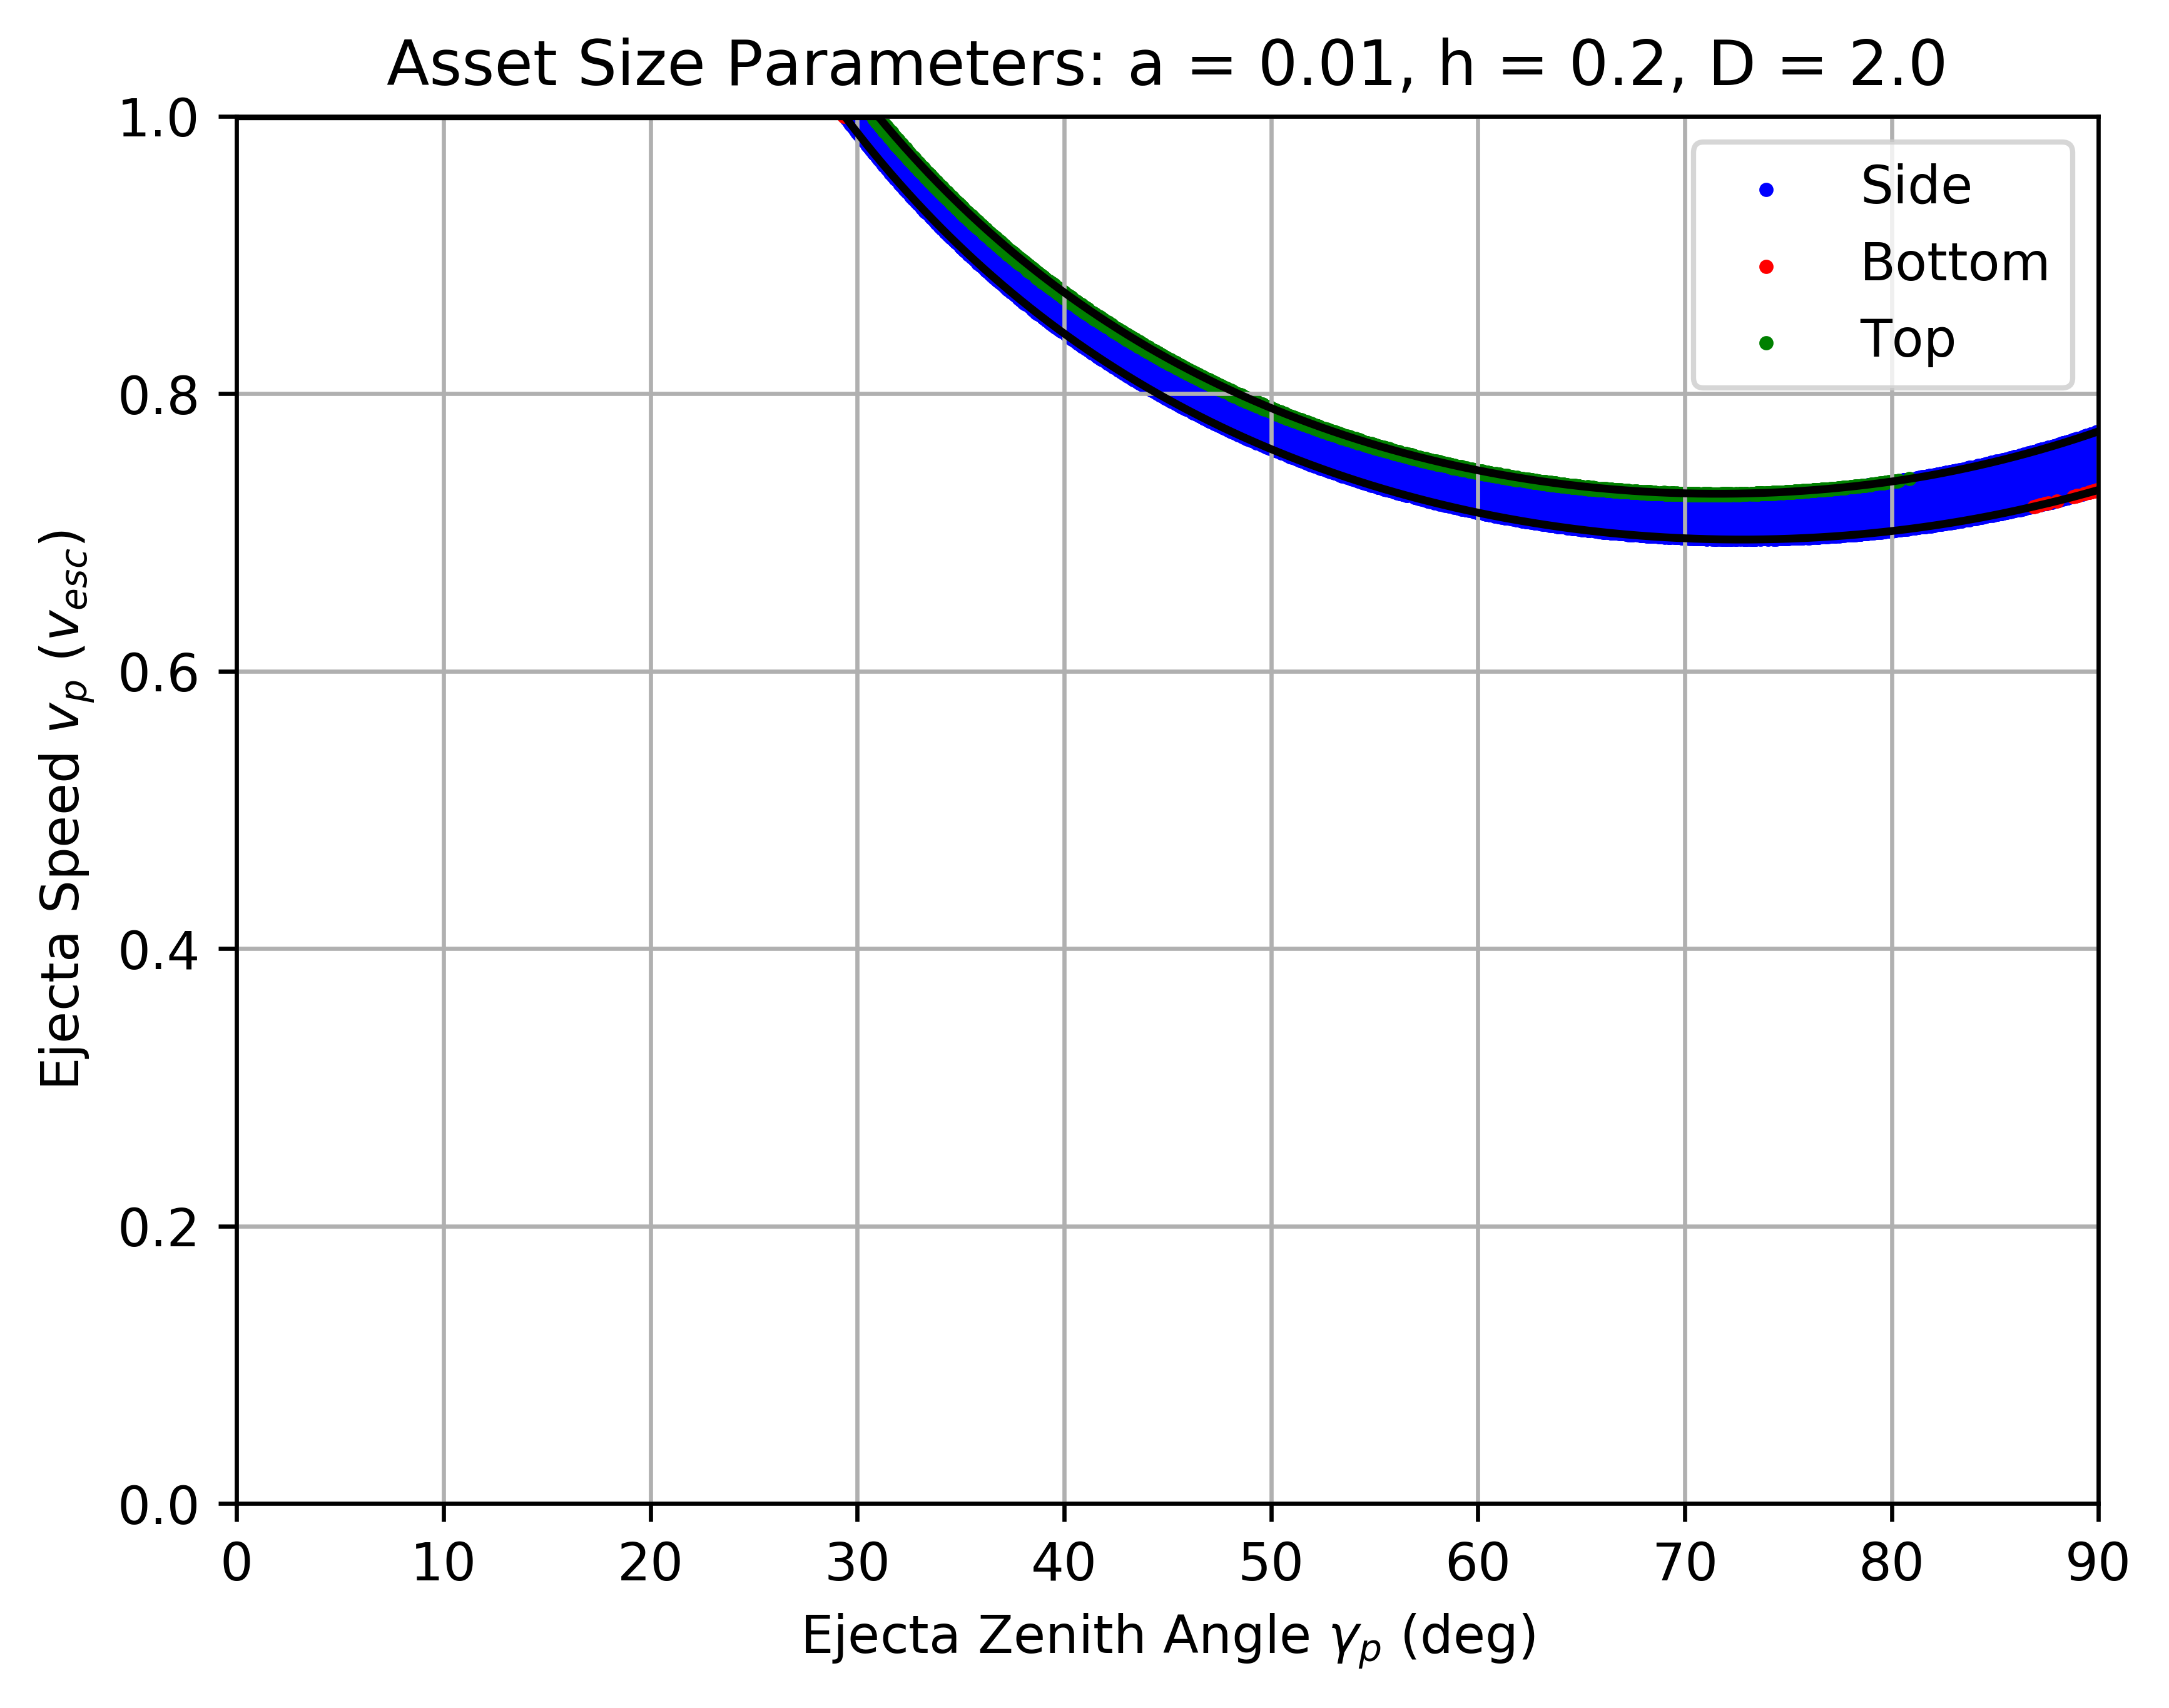
\includegraphics[width=.98\linewidth]{asset_speed_zenith_plot_1.100e+00_1.000e-02_2.000e-01_2.000e+00.png}  
		%\caption{Put your sub-caption here}
		\label{fig:sub-asset_speed_zenith_h2_10}
	\end{subfigure}
	\begin{subfigure}[t]{.32\textwidth}
		\centering
		% include fourth image
		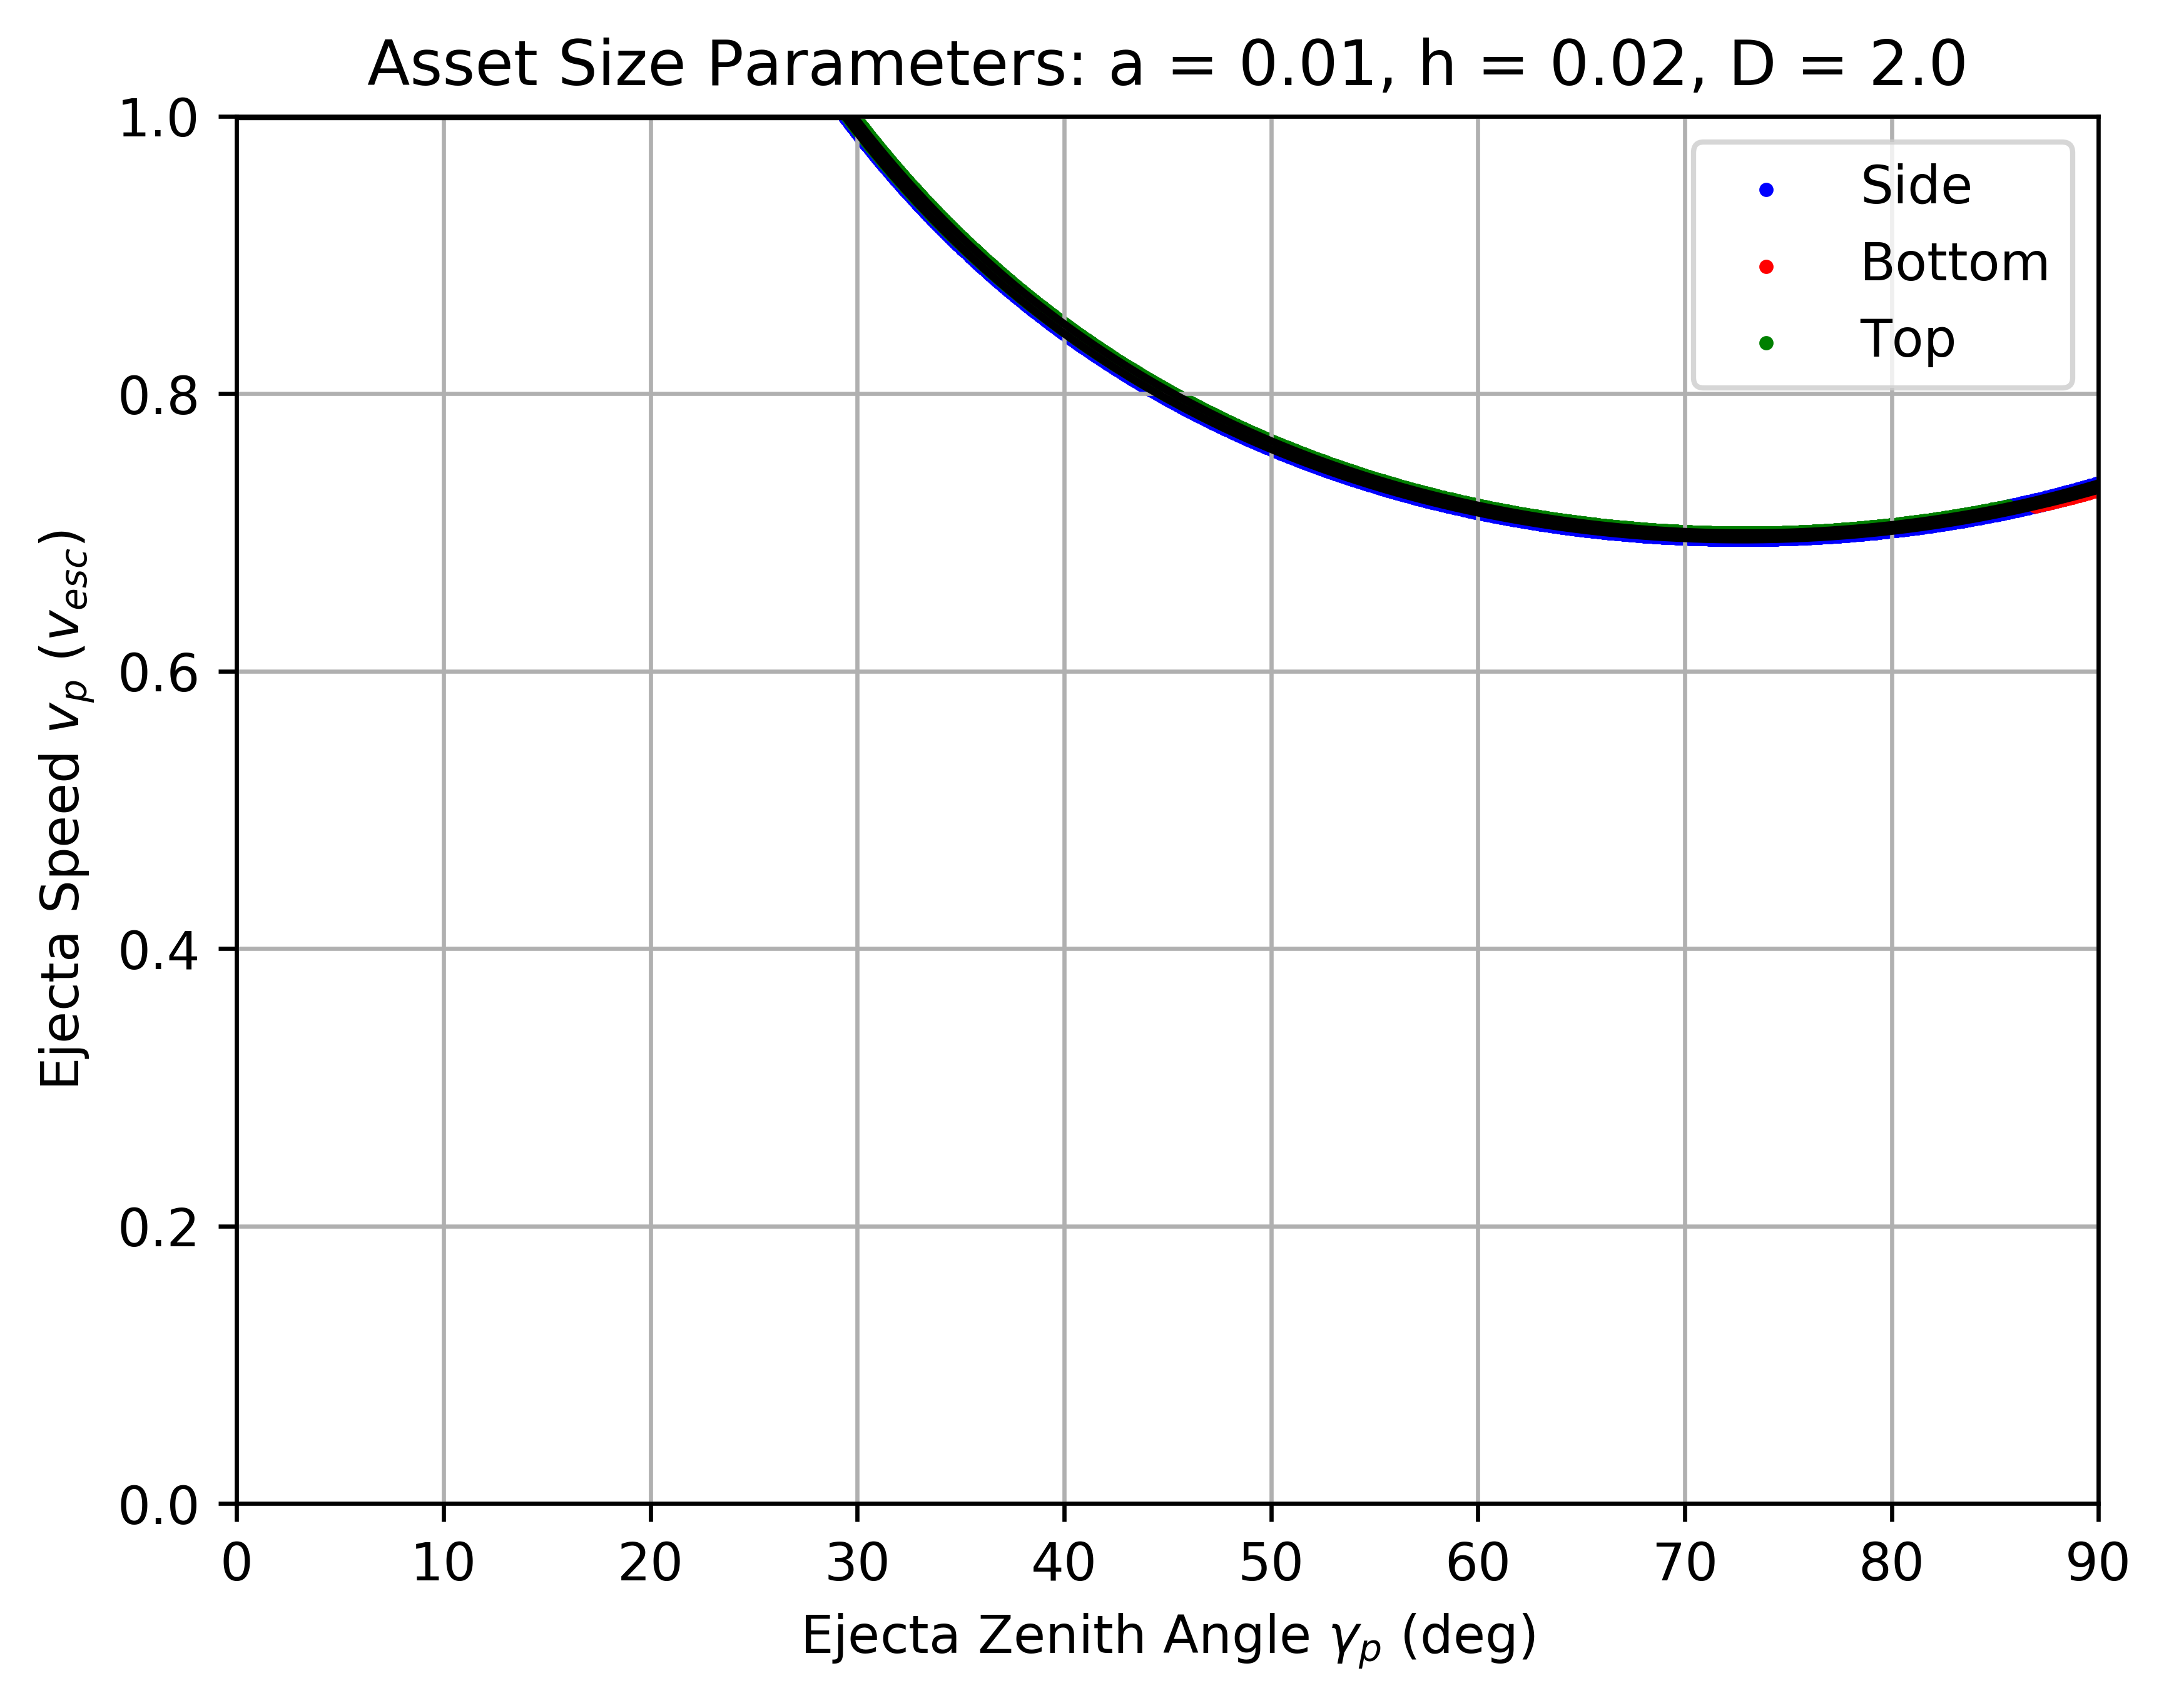
\includegraphics[width=.98\linewidth]{asset_speed_zenith_plot_1.100e+00_1.000e-02_2.000e-02_2.000e+00.png}  
		%\caption{Put your sub-caption here}
		\label{fig:sub-asset_speed_zenith_h2_11}
	\end{subfigure}
	\begin{subfigure}[t]{.32\textwidth}
		\centering
		% include fourth image
		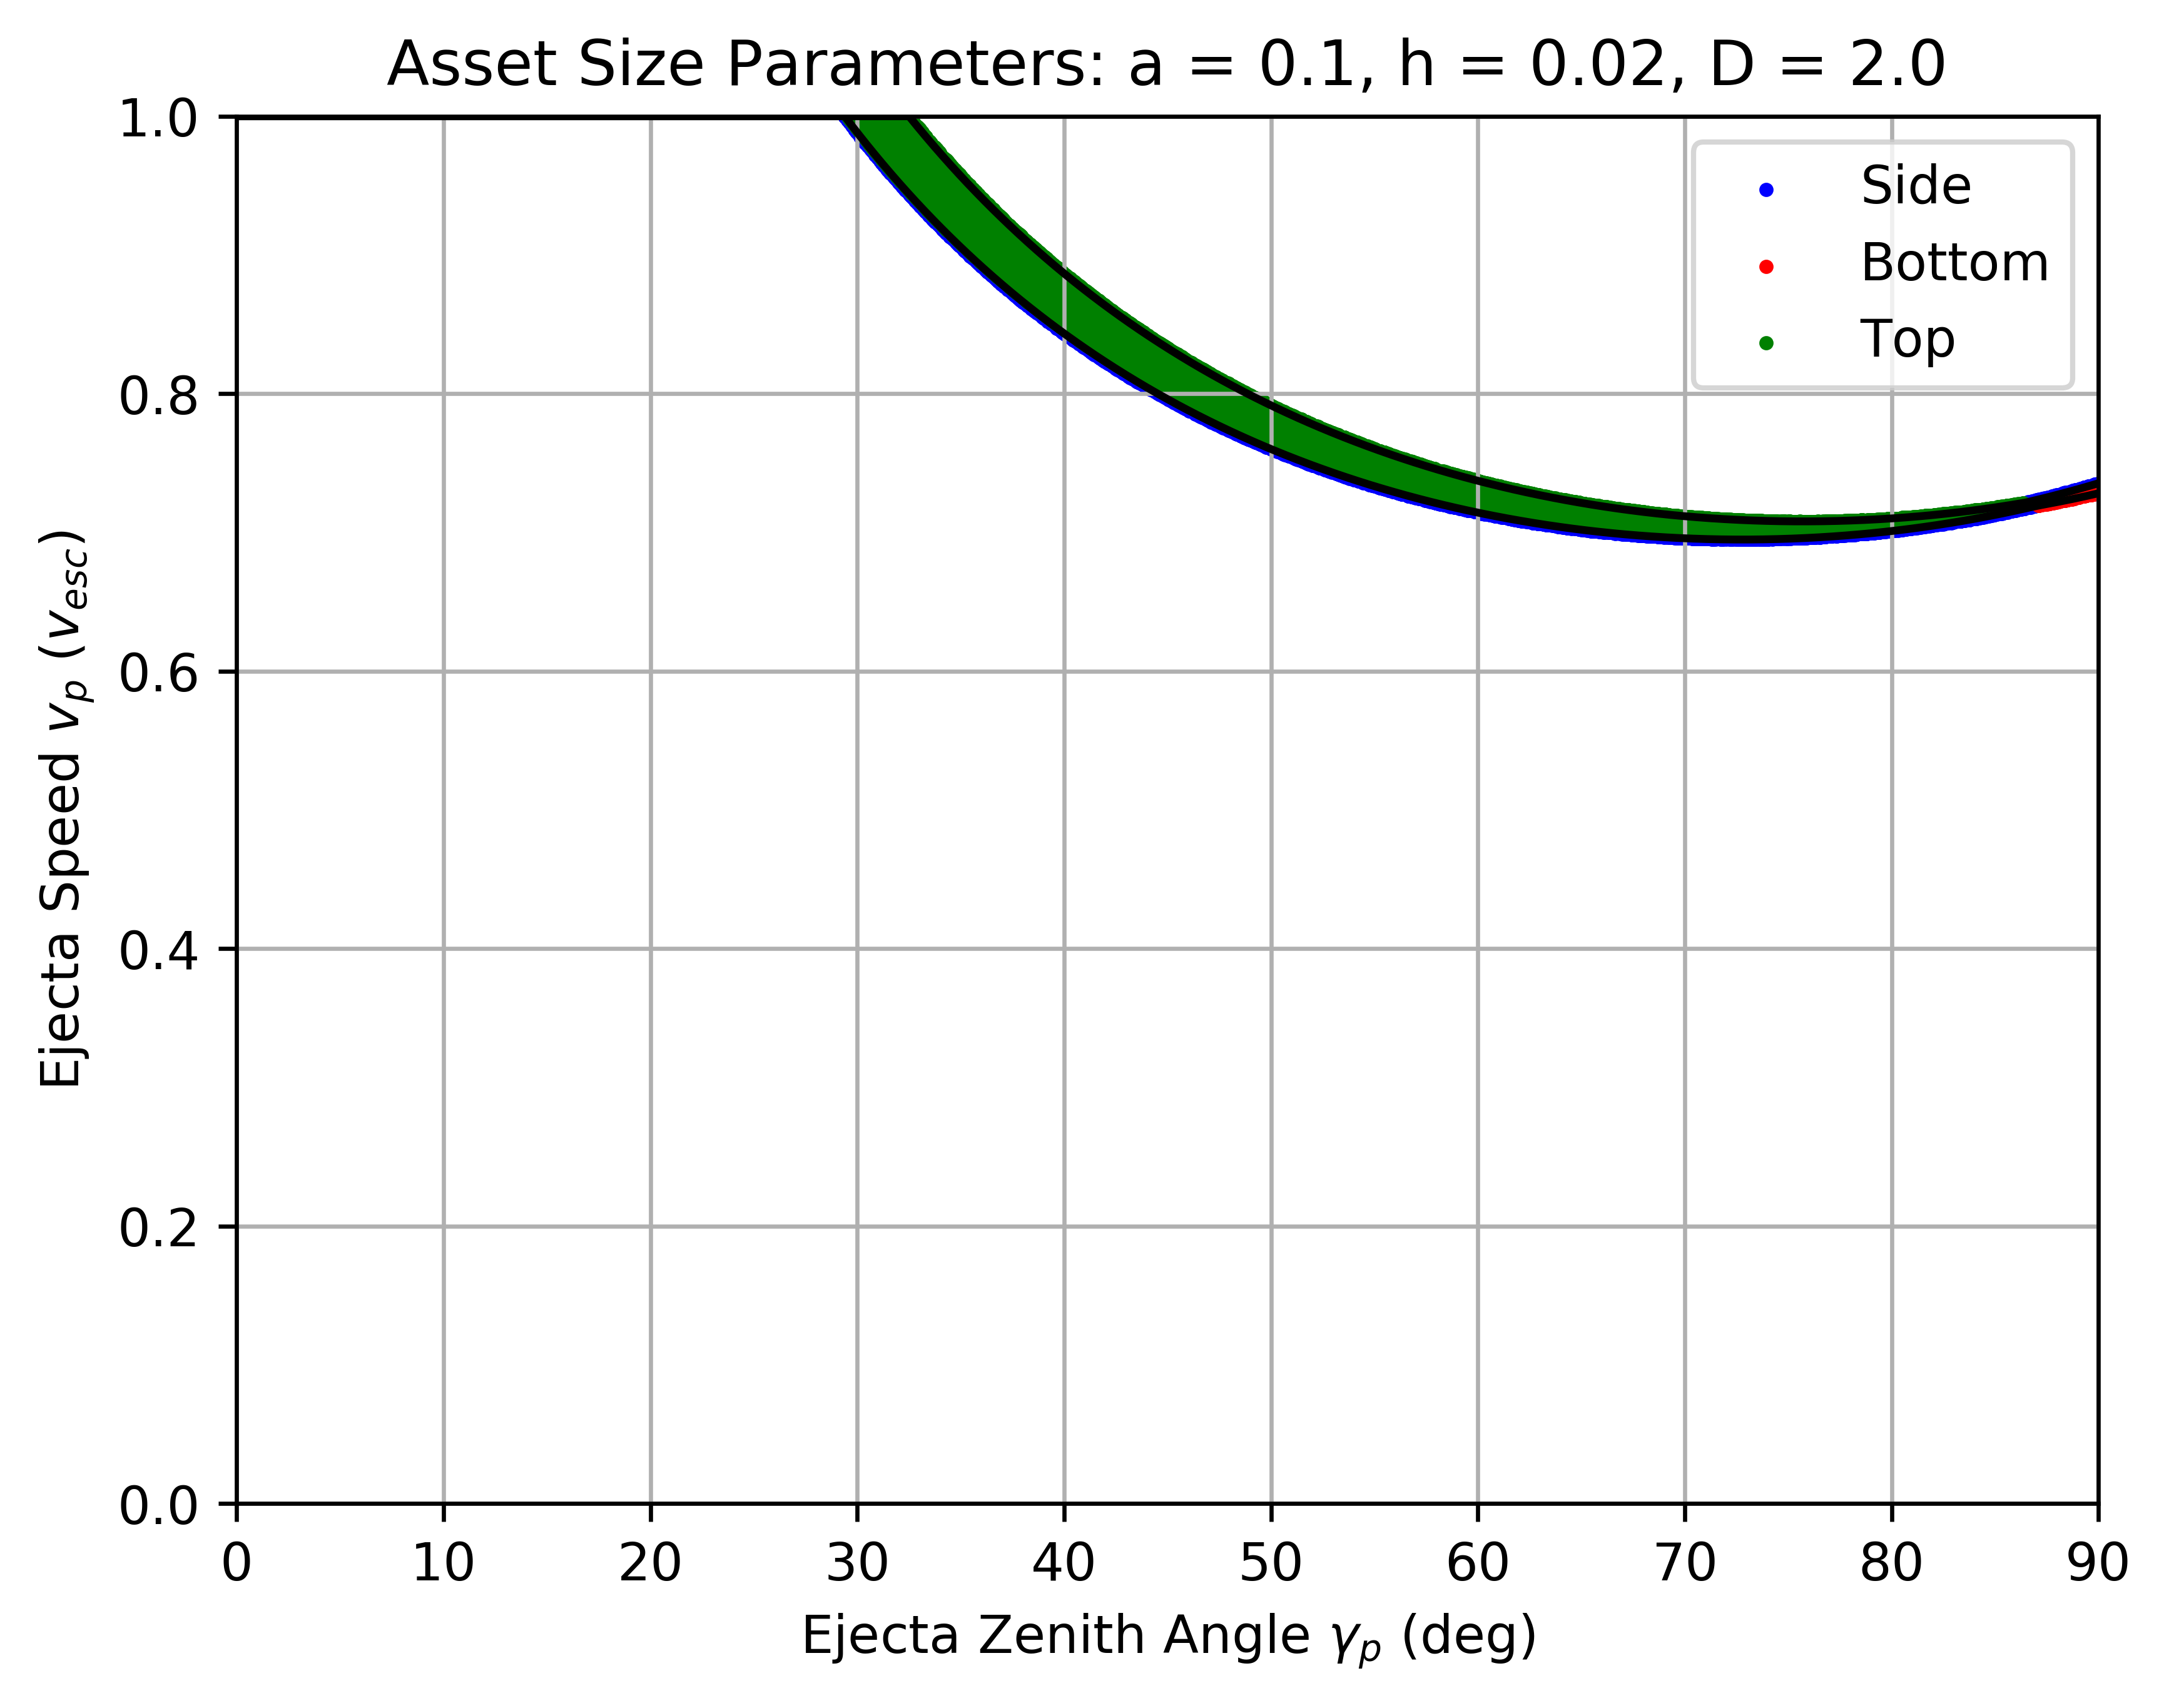
\includegraphics[width=.98\linewidth]{asset_speed_zenith_plot_1.100e+00_1.000e-01_2.000e-02_2.000e+00.png}  
		%\caption{Put your sub-caption here}
		\label{fig:sub-asset_speed_zenith_h2_12}
	\end{subfigure}
	
	\caption{A matrix of plots showing the ejecta hitting a cylindrical asset (in a plane intersecting the cylinder's symmetry axis) with a height above the surface of $0.1 r_m$ for various asset sizes and crater-to-asset distances. Each plot gives three colors for the ejecta hitting the side (blue), bottom (red), and the top (green) as a function of initial ejecta speed $v_p$ vs.\ initial ejecta zenith angle $\gamma_p$.}
	\label{fig:asset_speed_zenith_comparison_h2}
\end{figure}

\clearpage

%%%%%%%%%%%%%%%%%%%%%%%%%%%%%%%%%%%%%%%%%%%%%%%%%%%%%%%%%%%%%%%%%%%%%%
\subsection{Ejecta Speed-Zenith-Azimuth Sampling Algorithm}\label{ssec:Ejecta Speed-Zenith-Azimuth Sampling Algorithm}
There are two integration techniques that will combined in order to sample the ejecta speed-zenith phase space, importance sampling \citep[e.g., Section 9.7 of][]{kroese2013handbook} and stratified sampling \citep[e.g., Section 9.5 of][]{kroese2013handbook}.

In general, let $I$ be the integral given by
\begin{equation}
I = \int g(x)dx.
\end{equation}

Using importance sampling, the integral $I$ can be approximated as
\begin{equation}
I \sim \frac{1}{n}\sum_{i=1}^{n}\frac{g(x_i)}{f_{\hat{x}}(x_i)},
\end{equation}
where $f_{\hat{x}}(x_i)$ is a probability distribution function close to $g(x)$.

The integral $I$ can also be approximated using stratified sampling as
\begin{equation}
I \sim \sum_{j=1}^{N_1}\frac{vol(M_j)}{N_{0,j}}\sum_{i=1}^{N_{0,j}}g(x_{ij}),
\end{equation}
where each subdomain $M_j$ has a volume $vol(M_j)$.

Combining the two integration techniques, the integral $I$ can be written as
\begin{equation}
I \sim \sum_{j=1}^{N_1}\frac{vol(M_j)}{N_{0,j}}\sum_{i=1}^{N_{0,j}}\frac{g(x_{ij})}{f_{\hat{x}(x_{ij})}}.
\end{equation}


In the case of computing the fraction of total ejecta $M$ that hits the asset from a particular crater $\mathcal{C}$, the integral $I$ will be assigned as $M$ such that
\begin{equation}
M(\mathcal{C}) = \frac{1}{2\pi}\int_{\mathcal{R}(v_p,\gamma_p; \beta_i), \Phi(\beta_i)} d\beta_i d\gamma_p dv \frac{dM(v_p,\gamma_p)}{dv} F(\gamma_p) G(\beta_i-\beta_{imp}),
\end{equation}
where examples of the region $\mathcal{R}(v_p,\gamma_p, \beta_i)$ are shown in Figures \ref{fig:asset_speed_zenith_comparison}, \ref{fig:asset_speed_zenith_comparison_h1}, and \ref{fig:asset_speed_zenith_comparison_h2}, $\frac{dM(v_p,\gamma_p)}{dv}$ is the differential of the total ejecta mass (i.e., Equation~\eqref{eq:dM/dv final}), $F(\gamma_p)$ is the ejecta zenith distribution (see Section \ref{sssec:Ejecta:Zenith Distribution}), and $G(\beta_i-\beta_{imp})$ is the ejecta azimuth distribution (see Section \ref{sssec:Ejecta:Azimuth Distribution}) with $\beta_{imp}$ as the impactor azimuth.

The speed-zenith subdomain $M_j$ is broken up into $d\gamma_{p,j}$ segments, such that the corresponding $dv_{p,j}$ segments are within a maximum delta sizes, i.e.\
\begin{align}
d\gamma_{p,j} = \gamma_{p,j+1} - \gamma_{p,j} &\le d\gamma{p,max},\\
dv_{p,j} = v_{p,j,max} - v_{p,j,min} &\le dv_{p,max}.
\end{align}
Two consecutive segments define a trapezoidal area given by four points, $(\gamma_{p,j}, v_{p,j,min})$, $(\gamma_{p,j}, v_{p,j,max})$,  $(\gamma_{p,j+1}, v_{p,j+1,min})$, and $(\gamma_{p,j+1}, v_{p,j+1,max})$, such that the area is given by
\begin{equation}
Area(M_j) = \frac{1}{2}(dv_{p,j} + dv_{p,j+1})d\gamma_{p,j}.
\end{equation}
The area $Area(M_j)$ also defines where the speed-zenith points will be sampled for the $j$-th region. A separate check must be done to make sure that speed-zenith point is valid since there is a linear interpolation done from the $i$-th segment to the $i+1$-th segment.

The azimuthal region $\Phi(\beta_i)$ is defined by $\beta_{max}$ given in Equation \eqref{eq:beta max}. The effective height of the cylindrical asset does not change as a function of azimuth. However, the effective radius does, so a sampling weight is introduced to prefer the larger effective radii. A cumulative distribution function $F_{\hat{\Phi}}$ is generated by the effective radius as a function of crater-to-asset distance $D_i$, asset radius $a_i = c_i/2$, and azimuth offset from direct line-of-sight from crater to asset $\beta_i$ (see Figure \ref{fig:FOV}). The corresponding probability distribution function is given by $f_{\hat{\Phi}}$, which is used in sampling the azimuth in addition to the weight.

Therefore, the fraction of total ejecta $M$ can be approximated as
\begin{equation}
M(\mathcal{C}) \sim \frac{1}{2\pi N_2}\sum_{k=1}^{N_2}\frac{G(\beta_k-\beta_{imp})}{f_{\hat{\Phi}}(x_k)}\sum_{j=1}^{N_1}\frac{vol(M_j)}{N_{0,j}}\sum_{i=1}^{N_{0,j}}\frac{\frac{dM(v_{p,ij},\gamma_{p,ij})}{dv} F(\gamma_{p,ij}) }{f_{\hat{\mathcal{R}}}(x_{ij})}.
\end{equation}
The sum over $i$ handles the samples for a given subdomain of the speed-zenith grid (uniform in $\mathcal{R}$), the sum over $j$ is for each subdomain of the speed-zenith grid for a given azimuth, and the sum over $k$ is for each sampled azimuth with a weight of $f_{\hat{\Phi}}(x_k)$ in $\Phi(\beta_k)$.


\end{document}